\chapter{Eulerian Structural Topology optimization}
\label{chap:2}
\minitoc
\begin{mdframed}[hidealllines=true,backgroundcolor=lightgray!20]
\section*{Résumé}
Dans ce chapitre le design des structures conduites par simulation est passé en revue. Cela nécessite de 3 briques fondamentales: 
\begin{itemize}
\item Le modèle d'analyse éléments finis.
\item Le calcul des gradients.
\item L'algorithme d'optimisation
\end{itemize} 
Ces composantes sont représentées par des diagrammes par blocs, pour décrire leur interaction dans la boucle de design. La méthode adjointe de calcul des gradients et les algorithmes d'approximation séquentielle convexe sont aussi passés en revue.
La méthode du Matériau Solide avec Pénalité (SIMP), représentant des approches Eulériennes d'optimisation topologique, est aussi décrite en détails. Pour cette méthode la solution est représentée par un champ de densité constant par élément de maillage. Les variables d'optimisation sont donc les pseudo-densités dans chaque élément fini dans la zone de design, qui peuvent prendre de valeurs entre 0 et 1. Ce qui corresponde aux propriétés du vide et du solide respectivement. Pour éliminer les densités intermédiaires dans la solution, une pénalité est appliquée à la loi d'interpolation du module de Young entre le solide et le vide. Cette formulation souffre de plusieurs problèmes numériques. Cependant ceux-ci peuvent être traités par des techniques de restriction. Une approche multi-maillage pour un calcul efficace de la matrice de filtrage a été proposée pour réduire le cout d'évaluation de la matrice de filtrage. Ensuite pour traiter des contraintes de stress dans l'optimisation topologique l'approche unifiée d'agrégation relaxation \cite{verbart2017unified} est passé en revue et implémentée. Dans la dernière section de ce chapitre nous montrons l'application de l'approche SIMP au problème de design du mât et des attaches moteur. Des contraintes de symétrie de la solution et plusieurs cas de chargement sont également considérés.
\end{mdframed}
Design activity is a complex human activity that relies on both quantitative and qualitative judgment. A product will be the consequence of several decisions that are made to respect legal, environmental, safety and economic requirements. Moreover generally speaking a product will be the "best" or at least satisfying with respect to its performances among some configurations.
So the first requirement for the design process is being able to generate and describe design configurations or candidates. The second requirement is being able to evaluate the performance of a given candidate. Then the ranking of all configurations is made using one or several criteria.
The concept of best design depends on the particular criterion chosen for ranking different configurations. Moreover these criteria depend on the decision maker's point of view. In fact performance depends on the particular level at which the design choice is made. For example in complex systems, the design choice that would benefit the most a particular component could be detrimental for the whole assembly's performance\footnote{For instance in aircraft many subcomponents need to be designed. Changing the design of one subcomponent will have an impact on the load path definition  through other subcomponents. For this reason in the design loop finite element analysis are adopted to compute the load passing through each subcomponent interface.}. The person charged of making the choice about design, his position and his company could also have an impact on the criteria. For instance the recurrent costs and product lifetime span could be of primary importance for the consumer. On the other hand manufacturing costs could be more important for the manufacturer. Once the performance or cost criteria are defined, and all requirements are listed the choice would be to select the design that maximizes a given performance while respecting design constraints. The most naive approach to the design problem, would consist in producing each one of the design variants, test them and to selecting the best among them. This approach is of course impractical, expensive and incompatible with nowadays' economic reality. That's where modeling and simulation take their place. A model is any virtual or material abstraction of a given system that tries to predict its physical behavior with respect to particular operating conditions. This large definition can include any kind of simulation, or prototype that can be used to make a prediction on the configuration's behavior. It must be underlined that any model is only an abstraction of a particular phenomenon and not the real one. Every time a model is built some assumptions have to be considered, restricting of course it's domain of applicability\footnote{With this term the author identifies the ensemble of all situations in which a model can be considered to behave closely to the real product}. Once a model is available the aforementioned approach could be used to select the best candidates among the proposed candidates. Still this approach is applicable only if an exhaustive list of candidates is available, the model is valid for each configuration and the time and computational resources needed to evaluate these configurations are consistent with the designer's means. To avoid such a brute force approach to design, optimization algorithms can be adopted to make automated choices that improve a given configuration. These algorithms can generate a sequence of improved designs, which are simulated until a convergence is attained. The discipline that deals with the interaction between the optimization strategy and structural simulation is called structural optimization. In this large discipline one can find several families of optimization approaches. These can be classified in base of design assumptions, design variables nature and model assumptions (\cite{bendsoe2003theory}) as:
\begin{figure}[ht]
\centering
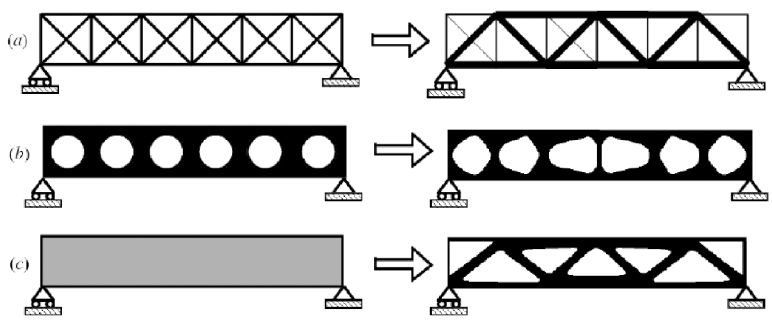
\includegraphics[width=10cm]{images/Ch2/a-Sizing-b-shape-and-c-topological-optimization-3}
\caption{(a) Sizing,(b) shape and (c) topology optimization \cite{bendsoe2003theory} }
\label{fig.2.1a}
\end{figure}
\begin{itemize}
	\item Size optimization: Often the design is mature, many modeling assumptions can be made. Thickness and cross section area typically are considered as design variables.
	\item Shape optimization: The design topology i.e. the number of holes in the structure is determined. Major modeling hypothesis can still be considered as true. The design variables are linked to the geometry in a freer manner. At this phase in fact both the contour of the domain and model can be modified by the design variables. 
	\item Topology optimization: the design maturity is low, some If any assumptions can be made, these are only about the neighboring components. Often the boundary conditions' positions are considered fixed. Other consideration can enforce the material to be inside a volume that is often referred to as design zone.
	The design variables are linked with material density inside the design zone. Depending on the approach this link can be more or less straightforward.
\end{itemize}
In figure  \ref{fig.2.1a} sizing, shape and topology optimization are applied to the same problem. In size optimization the solution is assumed to be a truss. Bar cross sections are design variables, model connectivity is unchanged during optimization. In shape optimization, the solution is assumed to have 6 holes and to be described by a solid continuum model. Holes geometries are varied during optimization but holes cannot collapse as this would change model connectivity. In topology optimization the only hypothesis about the solution  is that it can be represented by a solid continuum model. The number of holes and the connectivity of the solution are determined during the optimization.  
In this chapter we will focus mainly on topology optimization that is a very well established family of techniques in Structural Optimization, adopted for the determination of an optimal layout in preliminary design phases.
\section{Simulation driven design}
\label{sec:2.1}
In this section we want to introduce some basic concepts that we will use through the rest of this thesis. We base this section on the first chapter of \cite{papalambros2000principles}.
\subsection{Systems and Models representation}
Any product or design can be represented as a system, that can be defined as an assembly of subsystems or components that perform a function or a process, which results in an output. Any system or process can then easily be represented by the block diagram of figure \ref{fig.2.1}.
\begin{figure}[ht]
\centering
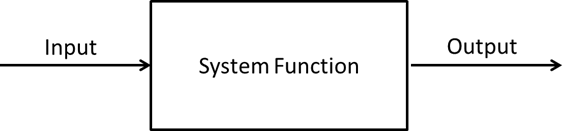
\includegraphics[width=8cm]{images/Ch2/Block_diagram_rep}
\caption{Block diagram representation}
\label{fig.2.1}
\end{figure}
For very complex products like aircrafts or gas turbine such a representation can help in understanding the flow of inputs and outputs between each component. On the other hand system block diagrams are subjective and they depend on the particular phenomenon of interest. Moreover the system representation also depends on the level of complexity at which a product needs to be represented. To predict the behavior of such a system, models have to be built. A rigorous definition of a model according to \cite{papalambros2000principles}:\\
\textit{A model is an abstract description of the real world giving an approximate representation of more complex functions of physical systems.}\\
In the same way one can distinguish between \textit{physical} models as the prototype that can emulate the real system's behavior with respect to some input and \textit{symbolic} models that can emulate the system's behavior through simulation. In this thesis we only refer to \textit{symbolic} models and in particular to \textit{mathematical} models:\\
\textit{A mathematical model represents a system by mathematical relations\cite{papalambros2000principles}}\\
Often this mathematical relation is explicitly available, or can be the result of a numerical computation.
With respect to optimization, variables can be divided into:
\begin{itemize}
\item \textit{Design Variables}: These quantities specify the design configuration. A design can be represented using such a variable to distinguish a design candidate from another.
\item \textit{Design Parameters}: These are quantities that identify the system's operating conditions. In structural models these can be identified with load and boundary conditions applied to the model.
\item \textit{Design constants}: 
These quantities are related to the physical phenomenon under study and cannot be altered. For example the gravity acceleration on the earth's surface. 
\end{itemize} 
This distinction is important because one can observe that the design of a system deals with the determination of \textit{Design Variables}, under specific working conditions determined by \textit{Design Parameters} and  \textit{Design constant} that are fixed for each design study.
\subsection {Analysis model}
As seen in chapter \ref{chap:1} structural FEMs are mathematical models that emulate the behavior of real structures under loading conditions. The input of such models will be the \textit{Design Variables} that identify the structure studied. The outputs of these models are important responses that can have a more or less direct link with the engineering requirements. FEMs can in fact be used to determine safety factors, displacements, and others. For the linear static analysis model, one can consider a multi-input$/$multi-output block diagram representation that takes as input the \textit{Design Variable} vector $\VectorVar{x}$ and reads in output the displacement vector $\VectorVar{U}$, through the model's relation. Here we introduce the notation of Matrix of Right Hand Side (RHS) vectors $\MatrixVar{F\left(\VectorVar{x}\right)}$ for multiple loads, where each column corresponds to a load case. Moreover we introduce $\MatrixVar{U\left(\VectorVar{x}\right)}$, for the corresponding solution vectors.
\begin{equation}
\label{eq2.1}
\MatrixVar{K\left(\VectorVar{x}\right)}\MatrixVar{U\left(\VectorVar{x}\right)}=\MatrixVar{F\left(\VectorVar{x}\right)}
\end{equation}
It should be noticed that both stiffness and load vectors can be a function of the configuration i.e. of the  \textit{Design Variable} $\VectorVar{x}$.
\begin{figure}[ht]
\centering
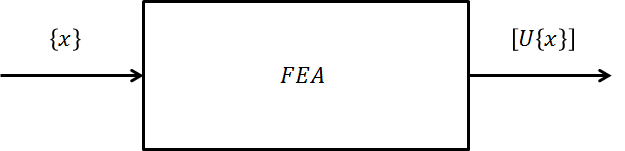
\includegraphics[width=8cm]{images/Ch2/Block_diagram_FEA}
\caption{FEA block diagram representation}
\label{fig.2.2}
\end{figure}
Moreover a FEA block hides several operations:
\begin{itemize}
\item The stiffness matrix assembly.
\item The right hand side vectors assembly.
\item The linear system solution per each right hand side vector.
\end{itemize}
This functional analysis allows a more detailed description of the FEA subsystem's block description c.f. figure \ref{fig.2.3}:\\
\begin{figure}[ht]
\centering
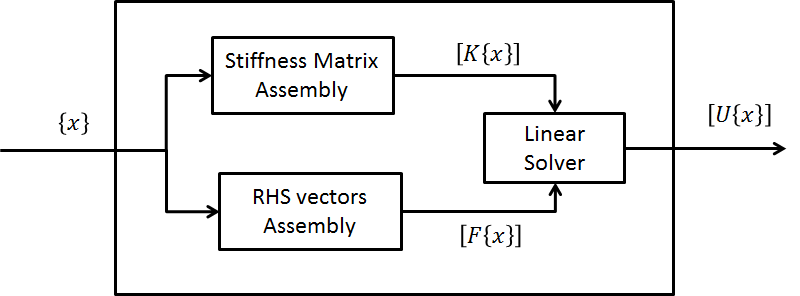
\includegraphics[width=8cm]{images/Ch2/Block_diagram_FEA_det}
\caption{FEA subsystem block diagram representation}
\label{fig.2.3}
\end{figure}
After displacements are computed, a post-processing is often needed to evaluate responses of interest that are needed for design selection.
The post processing block representation is shown in figure \ref{fig.2.4}. This system takes as input design variable's vector and the displacement vectors, and as output:
\begin{itemize}
\item Optimization cost functions $\VectorVar{o(\VectorVar{x})}$. In multi-criteria/multi-objective optimization problems we can have in fact several functions that we may want to minimize or maximize in the final design. Often we refer to a singular objective function as several techniques exist to transform a multi-objective problem into a single-objective one \cite{marler2004survey}.
\item The inequality constraint vector $\VectorVar{g(\VectorVar{x})}$. This vector contributes to the problem's definition through inequalities that have to be respected by the design candidate in order to be accepted.
\item The equality constraint vector $\VectorVar{h(\VectorVar{x})}$. This vector contributes to the problem's definition through equalities that have to be respected by the design candidate in order to be accepted.
\end{itemize} 
\begin{figure}[ht]
\centering
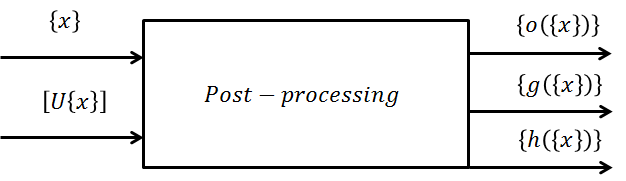
\includegraphics[width=8cm]{images/Ch2/Post_processing}
\caption{Post-processing block diagram representation}
\label{fig.2.4}
\end{figure}
\subsection {Optimization problem formulation}
Generally an optimization problem will be formulated as follows:
\begin{equation}
\label{nlp}
\begin{cases}
\min{\VectorVar{o(\VectorVar{x})}}\\
\textit{s.t.}\\
\VectorVar{x}\in D \subset \mathbb{R}^{n}\\
g_i(\VectorVar{x})\leq 0 & \forall i=1,2,...,m\\
h_j(\VectorVar{x})=0 & \forall j=1,2,...,l
\end{cases}
\end{equation}
where $D$ is a subset of $\mathbb{R}^{n}$ , $n$ is the number of design variables, $m$ and $l$ are respectively the number of inequality and equality constraints. Depending on the nature of $D$ one can make a first distinction between continuous and integer programming optimization problems. In the first case each design variable belongs to a closed interval in $\mathbb{R}$ which means that $D\equiv\lbrace \VectorVar{x} | \VectorVar{l_b}\leq\VectorVar{x}\leq \VectorVar{u_b}\rbrace$, where $\VectorVar{l_b}$ and $\VectorVar{u_b}$ are respectively design variable lower and upper bound vectors. For the second family of problems, the design variable belongs to a list of values.\footnote{Depending on the fact that one can sort or not design variable, one can also have the distinction between categorical or integer design variable} Most real life design problems include a combination of continuous and integer design variables. 
In this thesis we mainly focused on continuous optimization problems. A second distinction between optimization problems can be introduced for the number of criteria considered as simultaneous goals. One can consider either single or multi-objective design problems. As aforementioned the case where a list of goals needs to be considered can be carried out by the solution of a group of single objective problems. Another hypothesis we will consider for our responses is that they will be regular at least up to the first derivative with respect to the design variables. This hypothesis allows the use of efficient gradient based techniques for the optimization problem solution. 
 
\subsection {Optimum characterization}
A first important question about an optimization problem is about the existence of an optimal solution. In fact the feasible space, i.e. the space of solutions that simultaneously satisfy all constraints in the problem, can degenerate to a void space. Let's consider a 2D example where the design vector $\VectorVar{x}\equiv\VectorVar{x_1,x_2}^T$ has to solve the following optimization problem:
\begin{equation}
\begin{cases}
\min(o(x_1,x_2))=x_1+x_2\\
g_1(x_1,x_2)=\frac{x_1^2}{a^2}+\frac{x_2^2}{b^2}-1\leq 0\\
g_2(x_1,x_2)=c-(c+x_1)x_2\leq 0\\
0\leq x_1\leq 1\\
0\leq x_2 \leq 1
\end{cases}
\end{equation}
where $a,b,c$ are parameters. For some choice of these parameters the feasible space can be void as it is shown in figure \ref{fig.2.1bb}. 
\begin{figure}[hbt!]
  \centering
       \subfloat[ \label{fig.2.1ba}]{%
                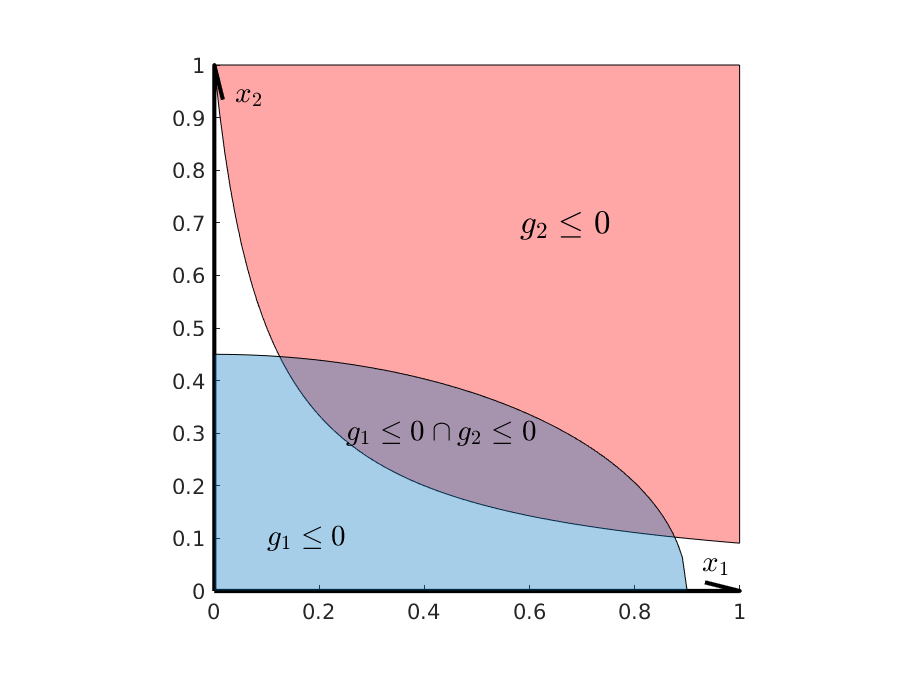
\includegraphics[width=0.5\textwidth]{images/Ch2/fdom.eps}
              }
       \subfloat[  \label{fig.2.1bb}]{%
         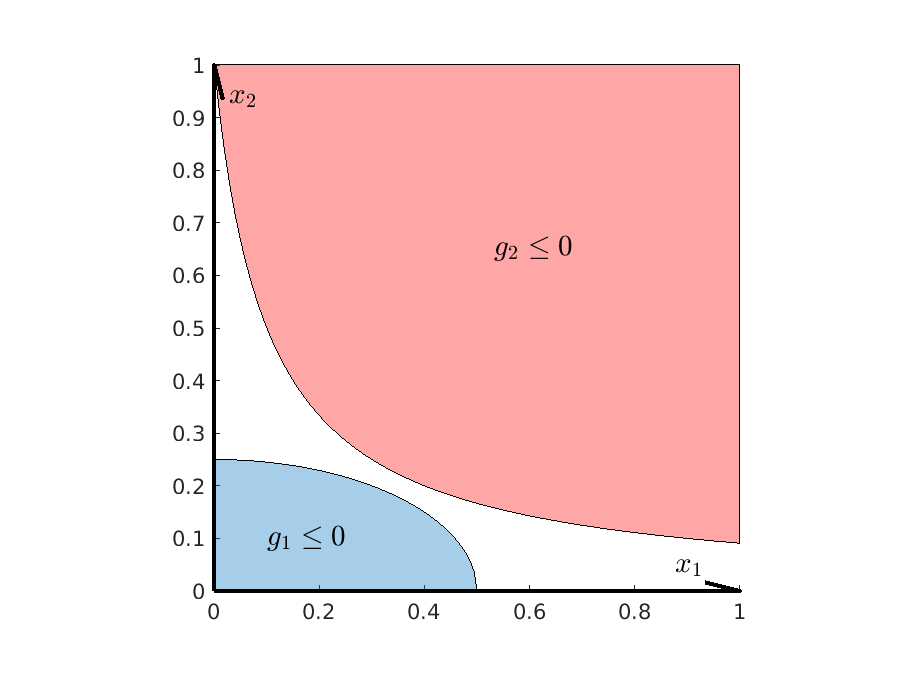
\includegraphics[width=0.5\textwidth]{images/Ch2/void_fdom.eps}
       }
       \caption{(a) Example of design domain representation for $a=0.9,b=0.45$ and $c=0.1$;(b)degenerate feasible domain for $a=0.5,b=0.25$ and $c=0.1$;.}
       \label{fig.2.1b}
     \end{figure}
In such cases the solution to the optimization problem will not exist. This situation often arises when dealing with antagonistic responses for constraints (for instance mass and maximum stress in a design). When this happens the only way of determining if a combination of requirements gives a void feasible design is by trials.\\
Another important property of an optimization problem is convexity.
A convex optimization problem is one whose objective and constraints are convex. It can be shown that the strictly convex optimization problem has only one solution and this solution is the global optimum of the optimization problem. For a non-convex problem we need to introduce the concept of local and global optimality. In fact a local optimum is a design configuration that is the best design for the goal function and that respects constraints, inside a small enough neighborhood of the solution. On the other hand a global optimum is the best design that satisfies the constraints over the whole design space and hence is the solution of the optimization problem.
We show this issue with a simple 1D example. 
Given the optimization problem:
\begin{equation}
\label{example_problem}
\begin{cases}
\min o(x)=\frac{3}{2}x^5-\frac{5}{2}x^3\\
s.t.\\
-\frac{3}{2}\leq x \leq \frac{3}{2}
\end{cases}
\end{equation}
The objective function is shown in figure \ref{fig.2.4b}.
\begin{figure}[ht]
\centering
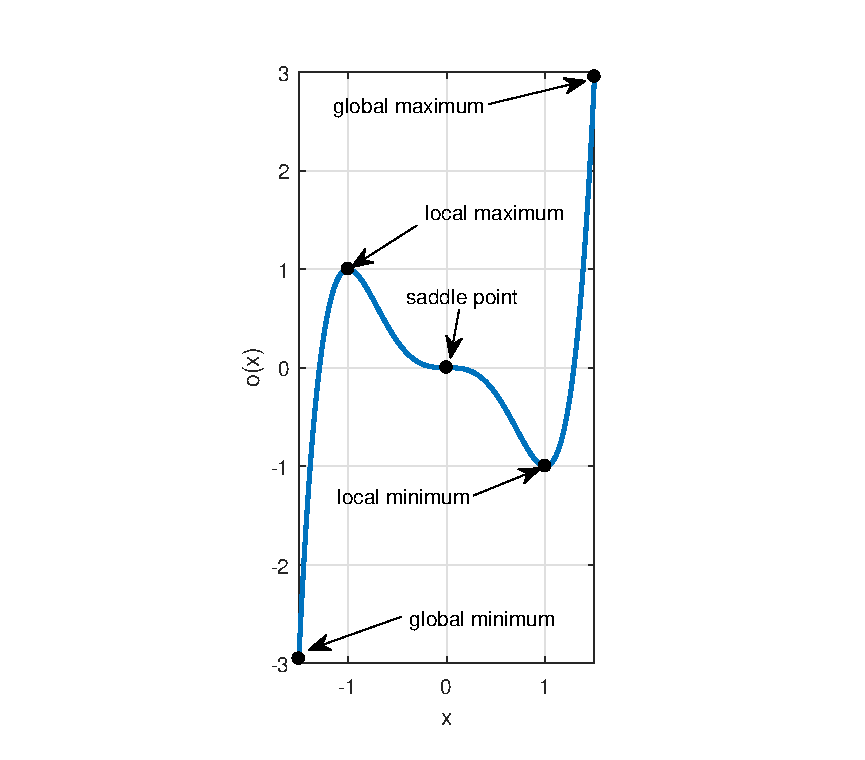
\includegraphics[width=12cm]{images/Ch2/example_minimum_maximum}
\caption{Optima characterization for the simple polynomial $o(x)=\frac{3}{2}x^5-\frac{5}{2}x^3$}
\label{fig.2.4b}
\end{figure}
We can observe that the point $x=1$ is a local minimum because it is possible to define a small interval around this point in which $o(x)$ is minimum. On the other hand $x=-\frac{3}{2}$ is the global minimum.
 Typically a non-convex problem (such as the one of equation \eqref{example_problem}) will possess several local optima but only one global optimum. In general, finding the global optimum can be considered as an insurmountable challenge for most optimization problems. For this reason, often one can only conclude that a design is an improvement of an existing one, but is not the best design ever achievable. 
With respect to constraints, an optimum can be either on the inside (interior optimum) or on the boundary (boundary optimum) of the design domain. The first situation arises when constraints are inactivated. This also implies that the unconstrained optimization problem (obtained ignoring all constraints) has the same solution as the constrained optimization problem. When this is not the case, the optimum will lie on the feasible design boundary. This implies that at least one constraint will be active so that $g_i=0$ for at least one $i\in\lbrace1,2,...,m\rbrace$. 
Here we can review necessary and sufficient conditions to determine if a point is a local minimum in a constrained problem \footnote{For the proof the interested reader can find it in \cite{papalambros2000principles}.}.
Given an optimization problem in the form of \footnote{Bound constraints on design variables can be considered as part of $\VectorVar{g(\VectorVar{x})}\leq \VectorVar{0}$}
\begin{equation}
\begin{cases}
\min o(\VectorVar{x})\\
s.t.\\
\VectorVar{h(\VectorVar{x})}=\VectorVar{0}\\
\VectorVar{g(\VectorVar{x})}\leq \VectorVar{0}
\end{cases}
\end{equation}
Given the Lagrangian of the problem:
\begin{equation}
\mathscr{L}(\VectorVar{x}):= o(\VectorVar{x})+\VectorVar{\lambda}^T h(\VectorVar{x})+\VectorVar{\mu}^T g(\VectorVar{x}) 
\end{equation}
where $\VectorVar{\lambda}\in \Real^l$ and $\VectorVar{\mu} \in \Real^m$ are Lagrangian multipliers
The necessary optimality conditions also known as \textit{Karush-Khun-Tucker (KKT) conditions} are:
\begin{equation}
\begin{cases}
\VectorVar{h(\VectorVar{x})}=\VectorVar{0}\\
\VectorVar{g(\VectorVar{x})}\leq \VectorVar{0}\\
\nabla o + \VectorVar{\lambda}^T\nabla h+\VectorVar{\mu}^T\nabla g=\VectorVar{0}\\
\VectorVar{\mu}\geq \VectorVar{0}\\
\VectorVar{\mu}^T\VectorVar{g(\VectorVar{x})}=0
\end{cases}
\end{equation}
when a point satisfies these conditions is said to be a KKT point and may not be a minimum since the conditions are not sufficient. Second order information is necessary to verify the nature of a KKT point:\\
\textit{ If a KKT point $\VectorVar{x_*}$ exists, such that the Hessian of the Lagrangian on the subspace tangent to the active constraints (equalities and inequalities) is positive-definite at $\VectorVar{x_*}$, then $\VectorVar{x_*}$ is a local constrained minimum.}\\
Coming back to our simple 1D example \eqref{example_problem} it is possible to show that $x_1=-\frac{3}{2}$,$x_2=-1$, $x_3=0$ and $x_4=1$ are KKT points. In fact being $\frac{do}{dx}=0$ for $x_2=-1$, $x_3=0$ and $x_4=1$ in all these points Lagrange multipliers associated with the bound constraints $x+\frac{3}{2}\leq 0$ and $-x+\frac{3}{2}\leq 0$, respectively $\mu_1$ and $\mu_2$ are both equal to 0.
Making the analysis of the Hessian of the Lagrangian (in this case $\frac{d^2 o}{dx^2}=30x^3-15x$ being all constraints inactivated) one can observe that: 
\begin{itemize}
\item $\frac{d^2 o}{dx^2}(-1)=-15$, so that $x=-1$ is a local maximum
\item $\frac{d^2 o}{dx^2}(1)=15$, so that $x=1$ is a local minimum
\item $\frac{d^2 o}{dx^2}(0)=0$, so that nothing can be stated on the point in $x=0$. Making an analysis of the third order derivative one can actually conclude that this KKT point is actually a saddle point.
\end{itemize}
For the point in $x=-\frac{3}{2}$ the second constraint is inactive so that $\mu_2=0$. On the other hand being $g_1=0$, $\mu_1$ can be different then zero (or not). Using the KKT conditions one can obtain $\mu_1=\frac{do}{dx}(-\frac{3}{2})=\frac{675}{32}>0$. Being the number of variables equal to the number of active constraints the plane tangent to the active constraint is degenerated to $\delta x=0$. In this case it is simpler to consider the fact that $o(x)$ is strictly monotone in the neighbor of $x=-\frac{3}{2}$. Moving from this point in the feasible space, the objective function will be increased.  This means that $x_1= -\frac{3}{2}$ is a local minimum. Moreover being $o(x_1)=-\frac{189}{64}< o(x_4)=-1$ one can conclude that $x_1$ is a global minimum. This kind of analysis makes the optimization problem solvable because both objective and constraint functions are analytic and inexpensive. Responses computed from the results of simulations can take much more time. That is why optimization algorithms need to be considered.
\subsection {Optimization solvers}
An optimization solver is a numerical strategy that can be adopted to generate a succession of designs that converge to at least a local optimum. Several approaches exist in the literature and can be chosen to treat a given numerical problem. Some important families of approaches can be determined depending on:
\begin{itemize}
\item The information about the derivatives of design responses needed by the optimizer to provide an improved design. One can say that an optimizer is of order $p$ if it uses up to the $p^{th}$ derivatives information to generate a new optimal candidates. A solver that uses only the function values is a 0 order method. On the other hand methods that use both the information of the function and the one of the gradients are considered first order methods and so on.
\item The priority given to design exploration with respect to the local optima refinement. A local optimization solver, aims at improving an initial design without any claiming about the global optimality. On the other hand global optimization solvers also explore the design space and often are proven to converge to the global optimum if the optimization iteration goes to infinity. 
\item The fact of adopting or not random processes inside the optimization loop. A deterministic solver starting from the same initial point will always fall in the same local minimum, when repeating the optimization process. In semi-stochastic solvers like evolutionary algorithms \cite{simon2013evolutionary} initializing the algorithm with the same starting individual (or population) the results can be different when repeating the optimization process. 
\item The fact of using the information coming from one individual or several individuals simultaneously. Surrogate assisted optimizations \cite{forrester2008engineering} are an example of approaches that use multi-design information. In these approaches approximations of the real objective and constraint functions are built on the basis of an initial design of experiments. Then the surrogates can be used to find new optimal candidates. Genetic Algorithms and other evolutionary algorithms also combine information coming from a population of individuals.
\end{itemize}
In this thesis we focus mainly on first order optimization solvers. In particular we considered Sequential Convex Programming algorithms such as the Method of Moving Asymptotes \cite{svanberg1987method,svanberg2002class}. From a block diagram point of view such optimizer can be seen as a system that takes as input the design variable vector, goal and constraint responses and their sensitivity at a given point and reads in output an improved design configuration (cf. figure \ref{fig.2.5}).
\begin{figure}[ht]
\centering
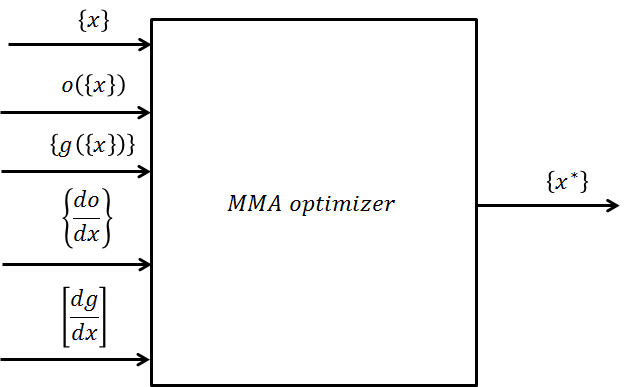
\includegraphics[width=8cm]{images/Ch2/Optimizer_block}
\caption{MMA optimizer block diagram representation}
\label{fig.2.5}
\end{figure}
In this representation we considered only inequality constraints inside the optimization problem. 
\subsection{Sequential Convex Programming algorithms}
In this subsection we describe in more details Sequential Convex Programming (SCP) \cite{fleury1993mathematical,zillober2004very,duysinx2009solution} general idea. In this family of approaches we can find convex linearization (CONLIN) algorithm \cite{fleury1986structural}, the Method of Moving Asymptotes (MMA) \cite{svanberg1987method,svanberg2002class}, and their variants like \cite{borrvall2001large,bruyneel2002family} and \cite{zillober2004very}.
Recently \cite{etman2012first} provided a review of SCP methods and discussed the fact that approximated approximation approach \cite{groenwold2010approximated} can be interpreted as diagonal quadratic subproblem in the spirit of the well-known SQP algorithms \cite{nocedal2006sequential}.
SCP algorithms are all based on reciprocal or reciprocal-like approximations of the original non-linear programming problem (c.f. equation \eqref{nlp}). They generate in this way  a series of convex non-linear programming subproblems. To generate such subproblems the following steps are followed:
\begin{enumerate}
\item Reciprocal intervening variables are replaced into first order Taylor series expansions of both objective and constraint responses 
\item The problem is made more convex that as aforementioned ensure the uniqueness of subproblems solution.
\item Often convexity is adjusted on the base of convergence history.
\end{enumerate}
When these approximations are built at the $k^{th}$ iteration of the optimization loop, the $P[k]$ subproblem has the following form.
\begin{equation}
\begin{cases}
\min_{\VectorVar{x}} \tilde{o}^{[k]}\\
s.t.\\
\VectorVar{\tilde{g}}^{[k]}\leq 0\\
\VectorVar{l_b}\leq \VectorVar{x}\leq \VectorVar{u_b}
\end{cases}
\end{equation}
The approximations adopted by MMA and CONLIN are separable (i.e. Hessian is diagonal). This means that efficient subproblem solvers can be adopted \cite{falk1967lagrange,fleury1979structural}. In order to ensure the convergence of $P[k]$ subproblem solutions $\VectorVar{x}^{[k]}_*$ to a solution (at least local) of the original problem (c.f. equation \ref{nlp}), either trust region \cite{alexandrov1998trust} strategies either conservatism frameworks \cite{svanberg2002class} can be adopted \cite{etman2012first}. In the first case the convergence is guaranteed introducing an allowed search domain around the iteration point $\VectorVar{x}^{[k]}$, i.e. the following constraint: 
\begin{equation}
\VectorVar{x}\in \mathscr{C}^{[k]}\equiv \lbrace -\delta^{[k]} \leq \VectorVar{x}-\VectorVar{x}^{[k]}\leq \delta^{[k]} \rbrace
\end{equation}
is added to the problem's formulation.
In the conservatism framework, the convexity of both cost and constraint approximations is adjusted to enforced convergence. Moreover the solution of each $P[k]$ subproblem $\VectorVar{x}^{[k]}_*$ in both cases may be rejected. In such case the subproblem is built again this time with a smaller trust region or with more conservative approximation until either convergence is reached or until the point  $\VectorVar{x}^{[k]}_*$ can be accepted as new iteration point $\VectorVar{x}^{[k+1]}$ \cite{svanberg2002class}.
 \subsubsection{The Method of Moving Asymptotes}
 Here we describe MMA derivation from intervening variable introduction and we report the implementation details of \cite{svanberg2007mma}.
 In this approach reciprocal intervening variables are introduced in the first order Taylor expansion. For several structural optimization problems it is known that this may yield nonlinear approximations of significantly better accuracy than linear \cite{etman2012first}. Therefore let’s consider the first order Taylor expansion of the objective function with respect to a generic intervening variables $y_i(x_i)$:
 \begin{equation}
 \label{taylor_exp}
\tilde{o}(\VectorVar{y})=o(\VectorVar{y}^{[k]})+\VectorVar{\frac{\partial o^{[k]}}{\partial y}}^T\left(\VectorVar{y}-\VectorVar{y}^{[k]}\right)
 \end{equation}
MMA makes the use of the following intervening variables:
\begin{equation}
\label{eq.211}
y_i=
\begin{cases}
\frac{1}{x_i-l_i^{[k]}} \quad \textit{if } \frac{\partial o^{[k]}}{\partial x_i}<0\\
\frac{1}{u_i^{[k]}-x_i} \quad \textit{if } \frac{\partial o^{[k]}}{\partial x_i}>0\\
\end{cases}
\end{equation}
where $l_i^{[k]}$ and $u_j^{[k]}$ are the lower and upper asymptotes. 
Equation \eqref{eq.211} substituted in \eqref{taylor_exp} gives:
\begin{equation}
\tilde{o}(\VectorVar{x})=\sum_{j=1}^N\left(\frac{p_j^{[k]}}{u_j^{[k]}-x_j}+\frac{q_j^{[k]}}{x_j-l_j^{[k]}}\right)+r^{[k]}
\end{equation}
where 
\begin{eqnarray}
\label{eq.2.13}
p_j^{[k]}=\left(u_j^{[k]}-x_j^{[k]}\right)^2\left(\frac{\partial o^{[k]}}{\partial x_j}\right)^+\\
\label{eq.2.14}
q_j^{[k]}=\left(x_j^{[k]}-l_j^{[k]}\right)^2\left(\frac{\partial o^{[k]}}{\partial x_j}\right)^-\\
r^{[k]}=o(\VectorVar{x}^{[k]})-\sum_{j=1}^N\left(\frac{p_j^{[k]}}{u_j^{[k]}-x^{[k]}_j}+\frac{q_j^{[k]}}{x^{[k]}_j-l_j^{[k]}}\right)\\
\left(\frac{\partial o^{[k]}}{\partial x_j}\right)^+=\max\left(0,\frac{\partial o^{[k]}}{\partial x_j}\right)\\
\left(\frac{\partial o^{[k]}}{\partial x_j}\right)^-=\max\left(0,-\frac{\partial o^{[k]}}{\partial x_j}\right)
\end{eqnarray}
It is useful to consider their visualization for a 1D example (c.f. figure \ref{fig.2.1c})
\begin{figure}[hbt!]
  \centering
       \subfloat[ \label{fig.2.1ac}]{%
                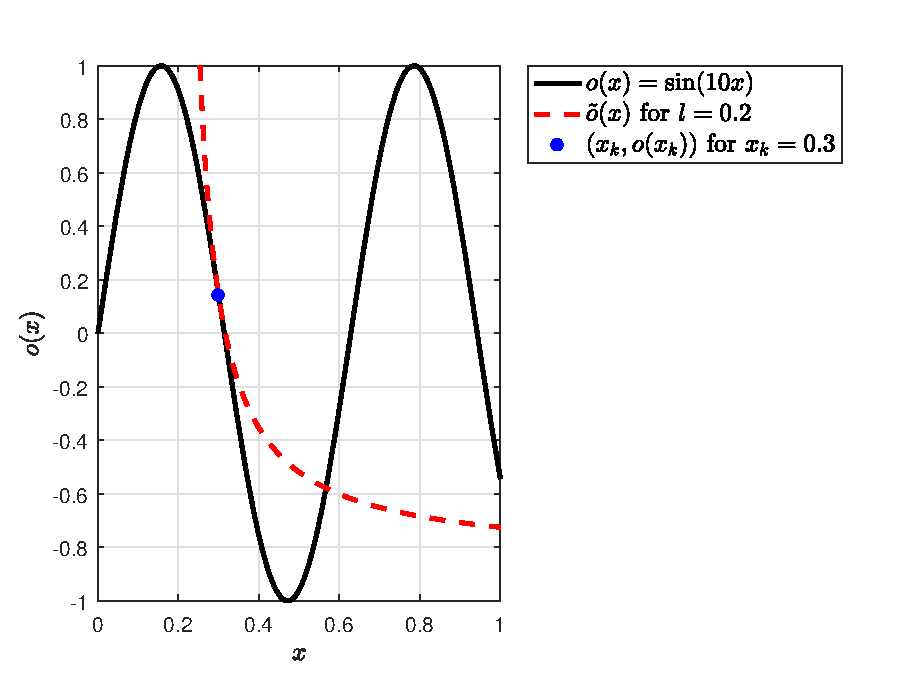
\includegraphics[width=0.5\textwidth]{images/Ch2/MMA_approx1.eps}
              }
       \subfloat[  \label{fig.2.1bc}]{%
         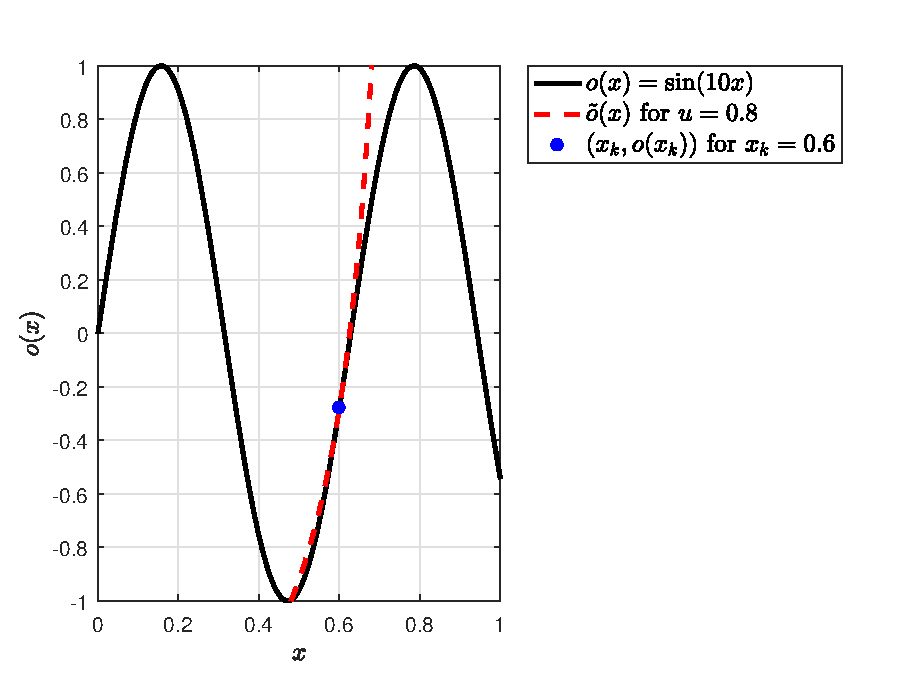
\includegraphics[width=0.5\textwidth]{images/Ch2/MMA_approx2.eps}
       }
       \caption{MMA approximations functions for a simple 1D example. The functions have different form depending on the derivative sign at the iteration point. The more asymptotes are close to the iteration point the more convex is the approximation function.}
       \label{fig.2.1c}
     \end{figure}
In such case we can recognize that the approximation function being first order approximation of the original function, shares with it its value and its derivative at the iteration point. It is also important to link the effect of asymptotes position on the approximation function and the impact that this can have on MMA conservatism. Let's consider again the elliptic feasible space described by:
\begin{equation}
g(x,y)=\frac{x^2}{a^2}+\frac{y^2}{b^2}-1\leq 0
\end{equation}
the asymptotes in each direction can here be put at a constant infinity norm distance from the current point:
\begin{eqnarray}
u_x-x_k=u_y-y_k=x_k-l_x=y_k-l_y=\Delta_a
\end{eqnarray}
The effect of the variation of $\Delta_a$ on the MMA approximation $\tilde{g}(x,y)$ is shown in figure \ref{fig.2.5b}.  
\begin{figure}[ht]
\centering
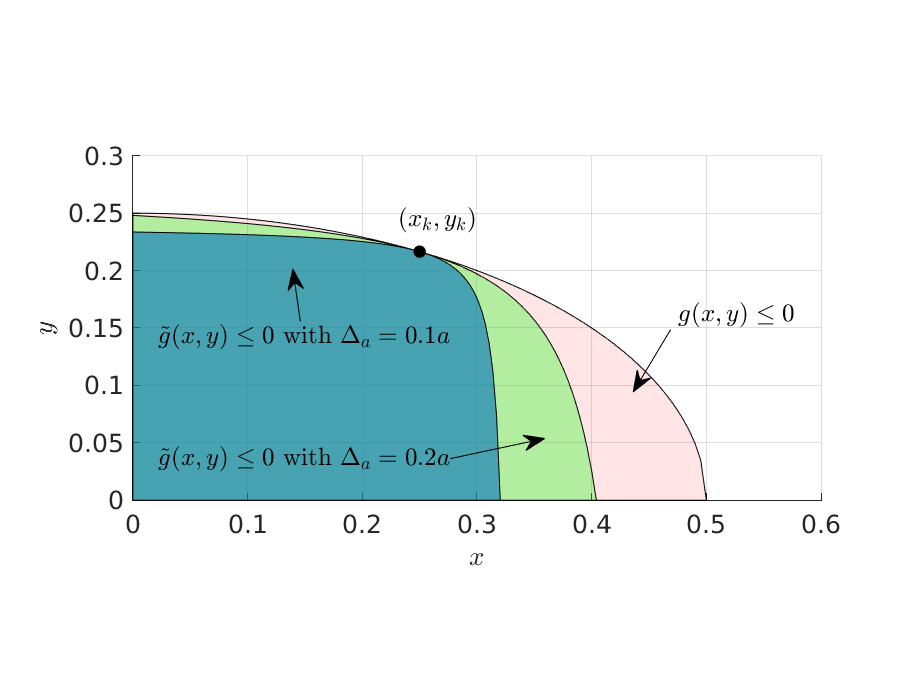
\includegraphics[width=12cm]{images/Ch2/MMA_conservatism}
\caption{Effect of the asymptotes distance $\Delta_a$ from the current point $(x_k,y_k)\equiv\left(\frac{a}{2},\frac{3}{2}b\right)$ on MMA approximation function $\tilde{g}(x,y)$ of the original constraint function $g(x,y)$  ($a=\frac{1}{2},b=\frac{1}{4}$). The smaller the distance, the higher is the approximation convexity, the smaller is the approximated feasible design space, the more conservative MMA will behave.}
\label{fig.2.5b}
\end{figure}
We can observe that smaller values of $\Delta_a$ reduce the size of the approximated feasible design space (i.e. $\tilde{g}(x,y)\leq 0$). In such way MMA solver can produce conservative subproblem optima that are more prone to satisfy true constraints (i.e. $g(x,y)\leq 0$). Understanding this principle is essential to correctly tune the solver parameters as it is described in appendix \ref{A1}.
It can be observed that the presented version of MMA actually fails encountering cost function or objective saddle points.
For this reason in the version of \cite{svanberg2007mma} equations \eqref{eq.2.13}-\eqref{eq.2.14} are modified as follows:
\begin{eqnarray}
p_j^{[k]}=\left(u_j^{[k]}-x_j^{[k]}\right)^2\left(1.001\left(\frac{\partial o^{[k]}}{\partial x_j}\right)^++0.001\left(\frac{\partial o^{[k]}}{\partial x_j}\right)^-+\frac{\rho_j}{u_{bj}-l_{bj}}\right)\\
q_j^{[k]}=\left(u_j^{[k]}-x_j^{[k]}\right)^2\left(0.001\left(\frac{\partial o^{[k]}}{\partial x_j}\right)^++1.001\left(\frac{\partial o^{[k]}}{\partial x_j}\right)^-+\frac{\rho_j}{u_{bj}-l_{bj}}\right)
\end{eqnarray}
where $\rho_j$ is a parameter, by default set to $10^{-5}$ that enforce strictly convexity of approximations \cite{svanberg2007mma}. The asymptotes position is adjusted during optimization to make MMA behavior more or less conservative. 
As default for the first two iterations, asymptotes positions are initialized as:
\begin{eqnarray}
l_j^{[k]}=x_j^{[k]}-0.5\left(u_{bj}-l_{bj}\right)\\
u_j^{[k]}=x_j^{[k]}+0.5\left(u_{bj}-l_{bj}\right)
\end{eqnarray}
in later iterations they evolve as:
\begin{eqnarray}
l_j^{[k]}=x_j^{[k]}-\gamma_j^{[k]}\left(x_j^{[k-1]}-l_j^{[k-1]}\right)\\
u_j^{[k]}=x_j^{[k]}+\gamma_j^{[k]}\left(x_j^{[k-1]}-l_j^{[k-1]}\right)
\end{eqnarray}
where
\begin{equation}
\gamma_j^{[k]}=\begin{cases}
0.7 \quad \textit{if} \quad \left(x_j^{[k]}-x_j^{[k-1]}\right)\left(x_j^{[k-1]}-x_j^{[k-2]}\right)<0\\
1 \quad \textit{if} \quad \left(x_j^{[k]}-x_j^{[k-1]}\right)\left(x_j^{[k-1]}-x_j^{[k-2]}\right)=0\\
1.2 \quad \textit{if} \quad \left(x_j^{[k]}-x_j^{[k-1]}\right)\left(x_j^{[k-1]}-x_j^{[k-2]}\right)>0
\end{cases}
\end{equation}
provided that this leads to values that satisfy:
\begin{eqnarray}
l_j^{[k]}\leq x_j^{[k]}-0.01\left(u_{bj}-l_{bj}\right)\\
\label{eqnMNAl}
l_j^{[k]}\geq x_j^{[k]}-10\left(u_{bj}-l_{bj}\right)\\
u_j^{[k]}\geq x_j^{[k]}+0.01\left(u_{bj}-l_{bj}\right)\\
\label{eqnMNAu}
u_j^{[k]}\leq x_j^{[k]}+10\left(u_{bj}-l_{bj}\right)
\end{eqnarray}
If any of this value is violated the corresponding $l_j^{[k]}$ or $u_j^{[k]}$ is put to the right hand side of the violated inequality \cite{svanberg2007mma}.
The asymptotes update strategy proposed in this approach in some cases become too aggressive with respect to constraint violations and sometimes diverge. For this reason globally convergent version of MMA was proposed in \cite{svanberg2002class}. Despite the risk of divergence, the simple "always accept" strategy is nevertheless frequently adopted and found to
be effective and efficient in many structural optimization applications \cite{groenwold2010conditional}. That is why such version was also considered in the present thesis even though specific tuning is proposed to enforce MMA conservatism (c.f. appendix \ref{A1}).
\subsection{Gradient adjoint evaluation}
 The MMA optimizer  takes as input all responses values and derivatives with respect to design variables, lower and upper bounds and gives as output the vector of the new optimal candidate. The success of MMA algorithm is therefore strictly linked to the accuracy of derivatives provided. 
 In order to efficiently compute response gradients many approaches can be found in the literature \cite{van2005review}\cite{martins2012short}. For explicit functions symbolic differentiations is possible by hand or using appropriate software like Maple, Mathematica or Matlab. Nevertheless for general algorithms it may be impossible to produce a closed form expression for the derivatives. 
 Finite differences are always an easily available option when a black box model is provided even though their efficiency is far from satisfactory. In fact several evaluations of responses are required and truncation error can also have an impact on the evaluation accuracy. Complex-step derivative approximation \cite{lyness1967numerical} are also efficient strategy that can be adopted when one have access to the core code of the provided response. The only requirement for this approach is that the model should be able to process complex input. As for finite difference, the number of design variable has a significant effect on the computational burden of this approach and therefore is impractical in the case of topology optimization problems. Algorithmic Differentiation (AD) \cite{griewank2000evaluating,naumann2012art} consists in the systematic application of differentiation chain rule to computer programs. It is as accurate as analytic method and can be much easier to implement \cite{martins2012short}. Still the most accurate and efficient methods available are analytic methods \cite{martins2012short}. In this family of approaches one can find both direct and adjoint approaches. The first is more advantageous for optimization problem where the number of design variables is smaller than the number of responses which sensitivities need to be computed, otherwise the adjoint is the most efficient strategy as the number of right hand side vector to be considered in the sensitivity evaluation is reduced. Being topology optimization characterized by a much greater number of design variables compared to the number of responses, here the adjoint evaluation is considered. 
  To this purpose let's consider a generic response $O(\lbrace x\rbrace,  \MatrixVar{U\left(\lbrace x\rbrace\right)})$ that depends both directly and  through the displacement vector on the design variables. 
  \begin{equation}
  \label{eq.2.43}
  \left\lbrace\frac{d O }{dx}\right\rbrace=\left\lbrace\frac{ \partial O }{ \partial x}\right\rbrace+\sum_{j=1}^{N_l}{\left[\frac{d U_j }{ d x}\right]\left\lbrace\frac{ \partial O }{ \partial U_j}\right\rbrace}
  \end{equation}
  By taking the derivatives of equations \eqref{eq2.1} (for the $j^{th}$-load case) one gets:
   \begin{equation}
   \label{eq.2.41}
   \frac{d\left[K(\lbrace x\rbrace)\right]}{dx_i}\lbrace U_j (\lbrace x\rbrace) \rbrace+\left[K(\lbrace x\rbrace)\right]\frac{d \lbrace U_j (\lbrace x\rbrace) \rbrace}{dx_i} = \frac{d\lbrace F_j(\lbrace x\rbrace) \rbrace}{dx_i} 
   \end{equation}
   Writing the product $\frac{d\left[K(\lbrace x\rbrace)\right]}{dx_i}\lbrace U_j (\lbrace x\rbrace) \rbrace$ as columns of the matrix $\left[\frac{dK}{dx}U_j\right]$ and $\frac{d\lbrace F_j(\lbrace x\rbrace) \rbrace}{dx_i} $ as the columns of the matrix $\left[\frac{dF_j}{dx}\right]$ one can also write:\footnote{Hereafter the dependency on $\lbrace x\rbrace$ and $\lbrace U_j (\lbrace x\rbrace) \rbrace$ is neglected for conciseness}
   \begin{equation}
   \left[\frac{d U_j }{ d x}\right]^T=\left[K\right]^{-1}\left(-\left[\frac{dK}{dx}U_j\right] +\left[\frac{dF_j}{dx}\right]\right)
   \end{equation}
   Defining the adjoint vector as:
   \begin{equation}
   \label{eq.2.46}
   \lbrace\beta_j  \rbrace=\left[K\right]^{-1}\left\lbrace\frac{ \partial O }{ \partial U_j}\right\rbrace
   \end{equation}
   One can finally rewrite equation \eqref{eq.2.43}:
   \begin{equation}
   \label{eq.2.47}
   \left\lbrace\frac{d O }{dx}\right\rbrace=\left\lbrace\frac{ \partial O }{ \partial x}\right\rbrace+\sum_{j=1}^{N_l}{\left(-\left[\frac{dK}{dx}U_j\right]^T +\left[\frac{dF_j}{dx}\right]^T\right)\lbrace\beta_j \rbrace}
   \end{equation}
   Such evaluation requires the a solution of static balance equations once per each load case and per each response. 
   This still represents an improvement for topology optimization problems where the number of design variables is much larger than the number responses times the number of load cases.
   \begin{figure}[ht]
   \centering
   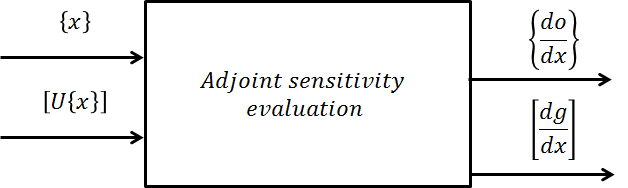
\includegraphics[width=8cm]{images/Ch2/Adjoint}
   \caption{Adjoint sensitivity evaluation block diagram representation}
   \label{fig.2.6}
   \end{figure}
    We can think of the adjoint evaluation of sensitivity as a model itself. This model takes as input the design variable's vector and the displacement vectors and reads in output the response sensitivity (cf. figure \ref{fig.2.6}).
    It must be noticed that some special responses, may not require any supplementary solution of static balance equations for the sensitivity evaluation. This is the case of compliance response. The compliance or the strain energy is commonly adopted as optimization objective in topology optimization. It is defined with respect to the j-th load case as:
    \begin{equation}
    c_j(\VectorVar{x})=\VectorVar{ U_j (\VectorVar{x})}^T \MatrixVar{K(\VectorVar{x})}\VectorVar{ U_j (\VectorVar{x})}=\VectorVar{ U_j (\VectorVar{x})}^T\VectorVar{ F_j (\VectorVar{x})}
    \end{equation}
   For such response one can easily compute:
   \begin{eqnarray}
   \VectorVar{\frac{\partial c_j}{\partial x}}=\MatrixVar{ \frac{\partial F_j}{\partial x}}^T\VectorVar{ U_j (\VectorVar{x})}-\MatrixVar{\frac{\partial K}{\partial x}U_j}^T\VectorVar{ U_j (\VectorVar{x})}\\
    \VectorVar{\frac{\partial c_j}{\partial U_j}}=\VectorVar{ F_j (\VectorVar{x})}\\
    \VectorVar{\beta_j}=\VectorVar{ U_j (\VectorVar{x})}
   \end{eqnarray}
   As aforementioned the adjoint vector being equal to the displacement vector, does not require any additional system solution for its evaluation. This results in a large computational economy for such design responses.
\subsection{Design loop \& human interaction} 
In the previous subsections we defined each block inputs and outputs, in this section we are going to show how these are connected into the design loop, and how the automated design loop is related with the human intervention.
\begin{figure}[ht]
\centering
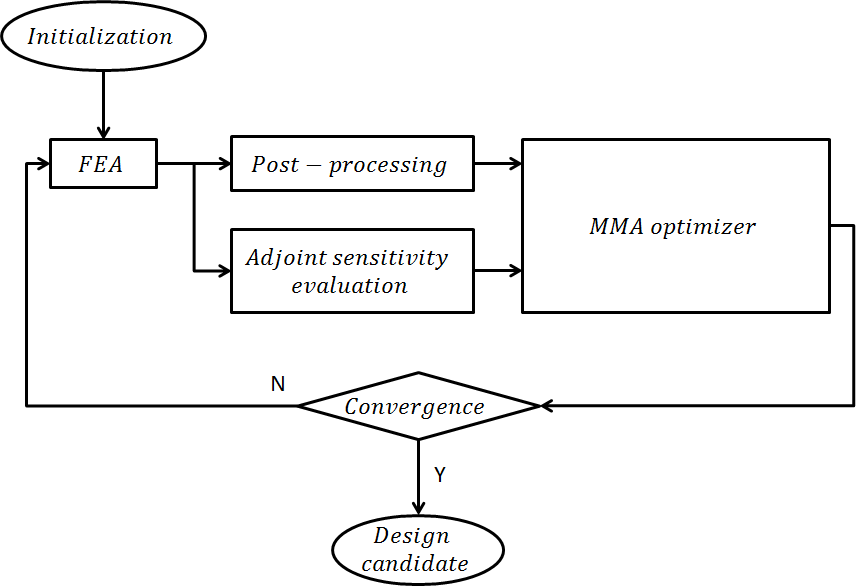
\includegraphics[width=10cm]{images/Ch2/optimization_loop}
\caption{Optimization loop block diagram representation.}
\label{fig.2.7}
\end{figure}
In figure \ref{fig.2.7} a complete structural optimization loop is illustrated. In the first phase the design loop has to be initialized with a starting guess design. This guess can be randomly selected. Anyway it is a good practice, when it is possible, to provide a starting guess that respects all constraints. This avoids useless optimization iterations required to reach the feasible domain. Another reasonable choice would consist in selecting as starting guess an existing configuration, so that the design could be improved. In this way an improvement should be guaranteed unless the initial design already is a local optimum. Other strategies require much more computational effort but try to deal with initial guess dependent problems. It is the case of multi-start strategies \cite{dixon1975towards}. The design loop can start once the initial guess choice is made. This design is tested within FEA block so that displacement vectors can be computed. Afterward Post-Processing and Adjoint sensitivity are applied to compute the optimization problem responses and sensitivities. Finally the optimization solver provides a new design candidate. At this point convergence has to be tested. Actually in some variants, convergence may be tested before MMA Optimizer gives a new candidate. Optimization convergence criteria can be based on the objective function's variation over several optimization iterations, can be based on the variation of the design variable's vector between consecutive iterations, on the number of iterations or on the verification of first order optimality conditions (KKT conditions).
If a solution is not attained, the iteration counter is increased and the new design candidate is sent to the FEA block.
If convergence is attained the optimization loop is stopped and the design can be considered as a candidate solution. Here we insist on the fact that automated optimization loop cannot provide optimal design without human intervention. 
Often the designer needs to make some decision about:
\begin{itemize}
\item The fact that a design candidate is an actual local minimum. In fact often a maximum iteration stopping criterion is reached, without reaching the other criteria (change of objective or change in the design vector less than a given tolerance). In this case either one accepts the design even if it is not an optimum, either the iteration convergence criterion has to be increased. In other more delicate situations the final design is not feasible even after a long convergence history. This can be due to the fact that the optimization problem is said to be over-constrained (there are no feasible solutions), or can be due to a bad choice of the initial guess. In more rare cases the optimizer was not correctly tuned to deal with the problem in hand or a scaling has to be introduced in the problem formulation. MMA optimizer needs special care for the choice of some parameters that make the difference on the final outcome.
\item The fact that a design candidate was correctly simulated. In other words if the design falls inside the model's validity domain. If this is the case one can either change the model's assumptions (for instance including nonlinearity in the model, changing the finite element order etc...) , either keep the same model but enforce the design to avoid such solutions changing both formulation and model. 
\item The fact that a design candidate is acceptable, i.e. is a manufacturable solution and is compliant with all requirements that can be identified on a quantifiable and qualitative level. This is a much more complex requirement for a design. Sometimes these manufacturing constraints may be considered during the optimization loop. It must be noticed that for this phase complex and expensive multidisciplinary simulations could be necessary to validate a design. 
\end{itemize}
The complete design loop described above is shown in figure \ref{fig.2.8}. One can observe that this procedure can be time consuming, but avoids the call to complex simulations that may not be required in the design loop as they  can be verified at the end of each optimization loop.
\begin{figure}[ht]
\centering
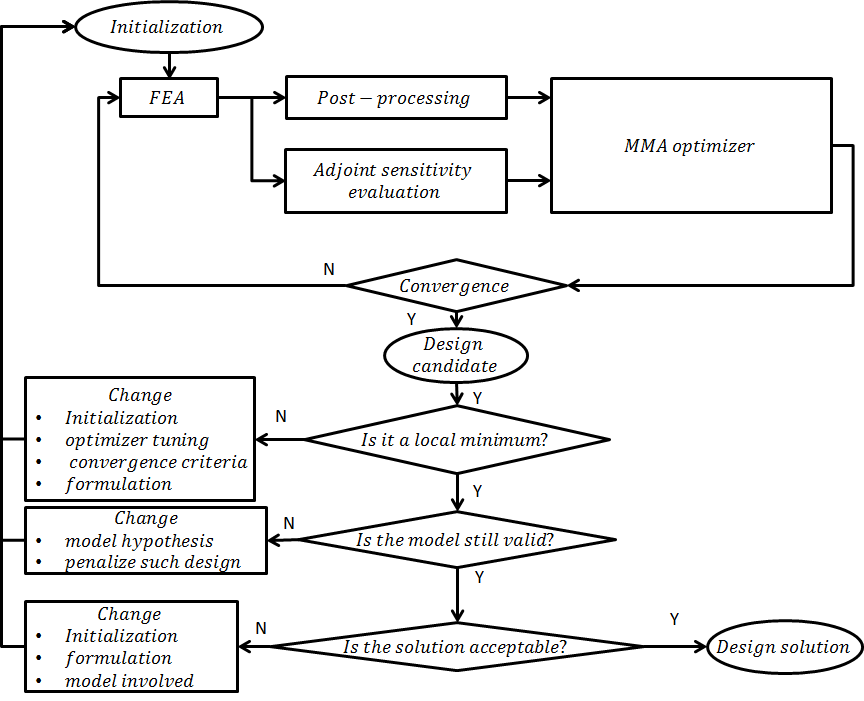
\includegraphics[width=10cm]{images/Ch2/design_loop}
\caption{Design loop block diagram representation}
\label{fig.2.8}
\end{figure}
Practically it can happen that some responses are still too expensive to be considered inside the design loop. In this case surrogate based optimization can represent a valid solution \cite{forrester2008engineering}.
\section{Density based topology optimization}
\label{sec:2.2}
In topology optimization, one seeks to achieve the design solution load path only knowing its design domain volume and its operating conditions. Since the pioneering work of Bendsoe and Kikuchi (1988) \cite{bendsoe1988generating}, topology optimization was developed and applied in several fields and physical problems. Here we focus on SIMP (Solid Isotropic Material with Penalization) \cite{bendsoe1989optimal}. This topology optimization approach is the most adopted in literature \cite{deaton2014survey} probably due to its simplicity and its robustness. Many other approaches could be considered as Level Set approach \cite{wang2003level}, Evolutionary Structural Optimization (ESO) \cite{xie1993simple} or biologically-inspired layout and topology optimization method \cite{kobayashi2010biologically}. The interested reader can find a review in \cite{deaton2014survey}. All these approaches show some advantages and shortcomings with respect to SIMP approach. For this reason, as a first attempt, we focused on SIMP. Future research could actually benefit from the investigation of other Eulerian approaches but are out of the scope of this dissertation.  
\subsection{Problem formulation}
In this method, the solution is described by a density field between zero and one that locally gives the information on the presence or the absence of material in terms of both mass and Young's modulus. 
A solution presenting intermediate density elements is always possible but is penalized by the power interpolation law used for the Young's modulus \cite{bendsoe1989optimal}.  Let us introduce a pseudo density field $x(\lbrace X_g \rbrace)$ in the design zone $\Omega$. This field has a physical meaning of presence or absence of material so that should take a value in $\{0,1\}$ reading 0 as absence of material and 1 as presence of material. For $x(\lbrace X_g \rbrace)=1$ one should use the value of local density and Young's Modulus of the real material $E$. In the case $x(\lbrace X_g \rbrace)=0$ the void can be simulated using a very soft material Young's Modulus $E_{min}$ that prevents stiffness matrix singularity and ill-conditioning. 
In order to use efficient gradient based optimization algorithms, the problem is commonly relaxed so that $x(\lbrace X_g \rbrace)\in [0,1]$. The physical interpretation of results presenting large regions characterized by intermediate density is not easy as they cannot be interpreted either as full material or void. For this reason, a simple penalization technique is commonly employed to prevent the optimization algorithm from converging on this kind of solutions. For this reason in the SIMP method \cite{bendsoe1989optimal}, the Young's modulus is written as a function of $x$ as:
\begin{equation}
\label{eq.6}
E(x)=E_{min}+(E-E_{min})x^p
\end{equation}
Where the penalty value $p>1$, penalizes the stiffness of intermediate densities.
The value of $p$ is usually set to 3 in order to get nearly black and white solutions. 
The Finite Element stiffness matrix assembly procedure will then use the local value of the Young's Modulus in order to compute the stiffness matrix. In our framework we considered the Young's modulus as constant in each finite element so that the element stiffness matrix can be computed using the value of $x$ in the element centroid $x_{el}$ and the unit modulus element stiffness matrix $\left[K_{el}^{(1)}\right]$:
\begin{equation}
\label{eq.7}
\left[K_{el}(x_{el})\right]=E(x_{el})\left[K_{el}^{(1)}\right]
\end{equation}
The design zone stiffness matrix is assembled summing the contribution of each element matrix in a classic FE style:
\begin{equation}
\label{eq.8}
\left[K_{DZ}(\lbrace x\rbrace)\right]=\overset{N_{el}}{\underset{el=1}{\bigoplus}}\left[K_{el}(x_{el})\right]
\end{equation}
Where $\bigoplus$ represents the assembly finite element operator and $N_{el}$ is the number of elements in the design zone.
Loads and boundary conditions are directly applied to the finite element model of the design zone. At this point for each material layout it is possible to compute the corresponding displacements vector. Historically topology optimization is associated with compliance minimization under volume constraints. This means that one looks for the stiffest material layout with respect to the loading conditions that fit inside the design zone within a given amount of material mass.
Formally we want to solve the following problem\footnote{Here we considered only one load case for brevity, the generalization to multiple load case will be detailed later.}:
\begin{equation}
\label{compl_formulation}
\begin{cases}
\min_{\VectorVar{0}\leq\VectorVar{x}\leq\VectorVar{1}} {\VectorVar{U(\lbrace x\rbrace)}^T\left[K_{DZ}(\lbrace x\rbrace)\right]\VectorVar{U(\lbrace x\rbrace)}} \\
\textit{s.t.}\\
\frac{\VectorVar{|\Omega_{el}|}^T\VectorVar{x}}{\VectorVar{|\Omega_{el}|}^T\VectorVar{1}}-v_f\leq 0
\end{cases}
\end{equation}
Where $\VectorVar{|\Omega_{el}|}$ is the element area vector, $\VectorVar{1}$ and $\VectorVar{0}$ are vector with the same size of $\VectorVar{x}$ whose values are all 1 and 0 respectively and $v_f$ is the value of allowable volume fraction. Optimization algorithms like the Optimality Criteria \cite{bendsoe1995optimization} or the aforementioned SCP algorithms \cite{svanberg1987method} are often adopted for the solution of this nonlinear programming problem. Once a design is determined, topology optimization solutions need to be re-interpreted and transformed in a realistic design. At this phase some model assumptions could be considered and further analysis and optimization could be performed until a final design is reached. For this second phase it is important to understand a solution's mechanical behavior and its global load path. Such considerations could come into account and the final solution could therefore be sensibly different from the original design determined in the topology optimization phase.
\clearpage
\subsection{Numerical difficulties \& density filter}
The optimization problem \ref{compl_formulation} suffers of several numerical difficulties \cite{sigmund1998numerical}:
\begin{figure}[ht]
\centering
\includegraphics[width=10cm]{images/Ch2/numerical_instabilities_TO}
\caption{Numerical instabilities in topology optimization \cite{sigmund1998numerical}, a) Problem definition b) solution with checkerboards, c) solution without checkerboards for a coarse mesh, d) solution with a refined mesh d) Example of problem with an infinity of local minima with the same stiffness and volume fraction}
\label{fig.2.8b}
\end{figure}
\begin{itemize}
\item \textit{Mesh dependence}: The solution of the optimization problem depends on the discretization adopted for the FEM. Mesh dependence is linked to the fact that the problem originating discretized  topology optimization (i.e. the continuum topology optimization problem with 0-1 density) doesn't have a solution (this problem is also known as nonexistence \cite{sigmund1998numerical}). Moreover the second issue related to this problem is the non-uniqueness of the solution. To deal with these difficulties several restriction techniques can be found in the literature. Here we report the perimeter control method \cite{ambrosio1993optimal,haber1996new}, the global gradient constraint \cite{bendsoe1995optimization}, the local gradient constraints \cite{niordson1983optimal} and the mesh independent filtering \cite{sigmund1994design,sigmund1997design} (for a larger review the reader can refer to \cite{sigmund2007morphology}).
\item \textit{Checkerboards}: The solution of \ref{compl_formulation} shows zones of alternated full and void materials in a checkerboard like fashion. It was shown by \cite{jog1996stability}  that this is due to FEM non convergence when representing such structures.
Several solutions have been proposed to avoid such problems, for instance:
Higher-order finite elements \cite{diaz1995checkerboard,jog1996stability}, the Patches \cite{bendsoe1993topology} and filtering \cite{sigmund1994design}. 
\item \textit{Local minima}: Changing algorithmic parameters one can find different solutions to the same problem, with the same FEM discretization. This is due to the optimization problem non convexity, and to the fact that optimizer adopted for topology optimization are most of the time local solvers. Global solvers are in fact less adapted to deal with such problems due to the large number of design variables. On the other hand continuation approaches can provide global or at least an improved solution. The idea is to start by solving a more convex problem (for instance for $p=1$) and then progressively move to the original non convex one (for instance progressively increasing the value of $p$), altering some parameters (penalty, filter radius or others) in both model and optimization formulation . Among classic approaches we can find the works of
\cite{allaire1993numerical,allaire1993topology}, strategies based on the perimeter constraint \cite{haber1996new}, on the value of the filter radius \cite{sigmund1997design,sigmund1997designb} or approaches based on the penalization of intermediate densities \cite{guedes1997prediction} .
\end{itemize}
\begin{figure}[hbt!]
  \centering
       \subfloat[ \label{fig2.14ab}]{%
                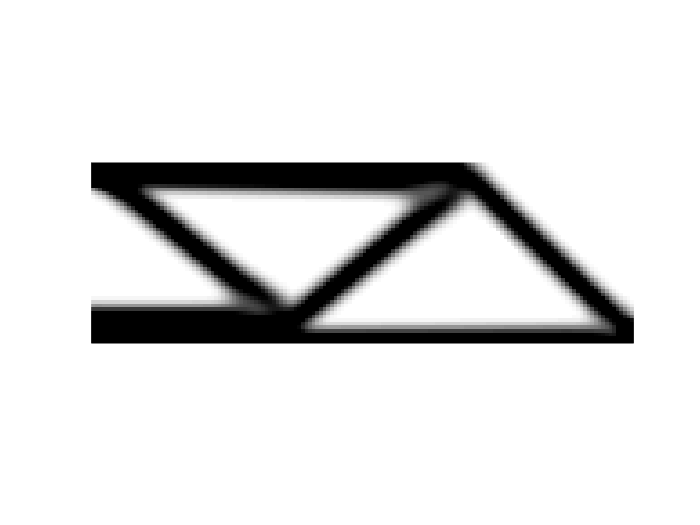
\includegraphics[width=0.5\textwidth]{images/Ch2/ft1}
              }
       \subfloat[  \label{fig2.14bb}]{%
         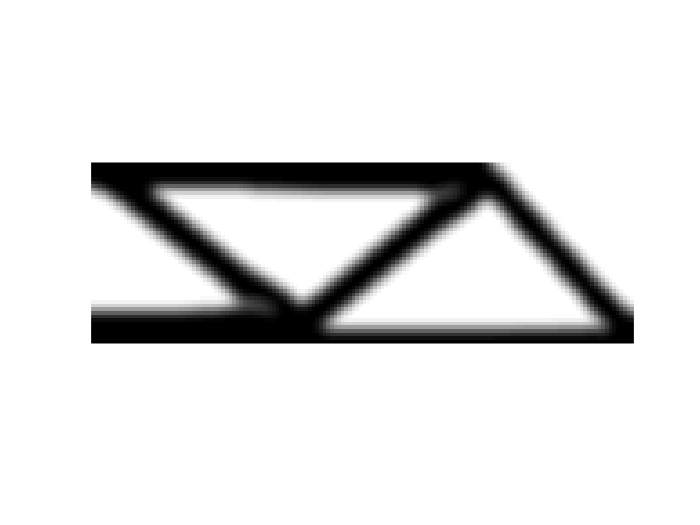
\includegraphics[width=0.5\textwidth]{images/Ch2/ft2}
       }
       \caption{a) sensitivity filters and b) density filters effect on the solution of a $150\times 50$ mesh MBB problem \cite{andreassen2011efficient}. }
       \label{fig2.14b}
     \end{figure}
In this thesis we adopted mesh independent density filters \cite{bourdin2001filters,bruns2001topology}.  As our meshes are non-uniform here we describe the procedure adopted for their computation.
 Typically mesh dependency and checkerboard related issues are solved using mesh independent filtering techniques.
 The density filter transforms the original density vector using an integral operator that in the continuous form is defined as:
 \begin{equation}
 \label{eq2.16}
x_{Phys}\left(\VectorVar{X_g}\right)=\int_{\Omega}{\kappa\left(\VectorVar{X_g},\VectorVar{\bar{X_g}}\right)x\left(\VectorVar{\bar{X_g}}\right)d\VectorVar{\bar{X_g}}} 
 \end{equation} 
 In this way even if the density distribution is rough, the filtered version defined by $ \VectorVar{x_{Phys}\left(\VectorVar{X_g}\right)}$ will inherit the smoothness of the kernel functions $\kappa\left(\VectorVar{X_g},\VectorVar{\bar{X_g}}\right)$.
 The latter is often chosen to be a linear hat kernel with radius $r$:
 \begin{equation}
 \kappa\left(\VectorVar{X_g},\VectorVar{\bar{X_g}}\right)=\hat{\kappa}\left(\VectorVar{X_g}\right) \max\left(0,1-\frac{\|\VectorVar{X_g}-\VectorVar{\bar{X_g} \|}}{r} \right)
 \end{equation}
 where:
 \begin{equation}
 \label{eq2.18}
\hat{\kappa}\left(\VectorVar{X_g}\right)=\left( \int_{\Omega}{\max\left(0,1-\frac{\|\VectorVar{X_g}-\VectorVar{\bar{X_g} \|}}{r} \right)d\VectorVar{\bar{X_g}}} \right)
 \end{equation}
 In a discretized version, these operations take the matrix form:
 \begin{equation}
 \VectorVar{x_{Phys}}=\MatrixVar{H}\VectorVar{x}
 \end{equation}
 Where the integral of equations \eqref{eq2.16}, \eqref{eq2.18} where replaced by Gauss numerical integrations using finite elements as support. 
 These techniques can be easily implemented for uniform structured meshes as is the case in \cite{andreassen2011efficient} and the majority of SIMP based topology optimization studies. 
 The fact of having 1x1 square element can be used to have a straightforward relationship between the element indexing and their neighbors center-to-center distances.  This is not the case for non-uniform unstructured meshes, as the ones considered here. In Talischi et al. \cite{talischi2012polytop} the difficulties induced by those cases are treated for 2D analysis with unstructured polygonal meshes. In particular it is shown that, to be more efficient, stiffness element matrices and  filter matrix can be assembled once for all before the optimization loop. In this study, 8-node 3D finite elements with tri-linear shape functions were employed and 8 Gauss points per element were considered for stiffness matrix assembly. On the other hand only one Gauss point was used in order to evaluate the filtering convolution integral. As a consequence, following the same implementation of \cite{talischi2012polytop} the filter matrix $\left[H\right]$ needs the evaluation of all distances $d_{ij}$ between each couple of element's centroid:
 \begin{equation}
 \label{e.11}
 H_{i,j} = \frac{max(0,| \Omega_j| (1-\frac{d_{ij}}{r})}{\sum_{j=1}^{N_{el}}max(0,| \Omega_j| (1-\frac{d_{ij}}{r})}
 \end{equation}
 Where $N_{el}$ is the element number in the design zone, $r$ is filter radius and $| \Omega_j|$ is the volume of $j^{th}$ element.
  The cost for this evaluation in terms of memory and CPUs time grows with $\frac{N_{el}^2-N_{el}}{2}$ . In \cite{talischi2012polytop} it is argued that this operation even if  expensive should be done once for all before the optimization loop and should not be a bottleneck for overall analysis. Nevertheless, when increasing the number of elements, this simple operation can encounter memory limits faster than stiffness matrix inversion. These limitations were also studied and tackled in the PDE filter proposed by Lazarov et al \cite{lazarov2011filters}, where instead of explicitly computing the filter matrix [H], the filtered field is found as the solution of a PDE problem. Such a solution involves a small memory cost, even if it requires the solution of a system of equations with the size the number of nodes, twice per iteration. These solutions are not very expensive for small problems. In fact they require a small effort compared to displacements evaluation. In this work we propose an alternative way of directly computing $\left[ H \right]$ that reduces the time needed for the computation of the filtering matrix, but still requires enough memory for the storage of $\left[ H \right]$. Note that for reasonably small values of the filtering radius, and for unstructured refined meshes, this proposed procedure appears advantageous. On the other hand for large values of the filtering radius and for the same kind of meshes the approach based on the PDE filter by Lazarov et al. \cite{lazarov2011filters} is to be preferred to reduce memory requirements. 
  It must be noted that $H_{i,j}$ is sparse since all distances superior to $r$ do not contribute to $H_{i,j}$ . We supposed to have a first mesh like the one in figure \ref{fig.7aa} on which we are able to evaluate all the distances between each element $d_{ij}$ and compare them to $r$. We also suppose that a refinement of this mesh can be obtained cutting each element into 8 as shown in figure \ref{f.7a}.
  \begin{figure}[hbt!]
  \centering
       \subfloat[ \label{fig.7aa}]{%
                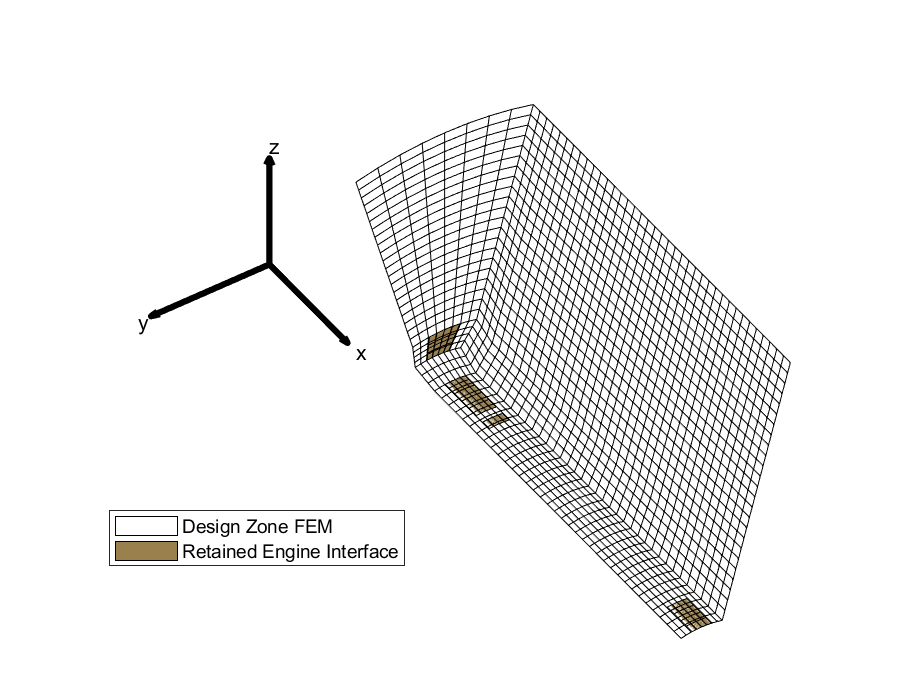
\includegraphics[width=0.5\textwidth]{images/Ch1/original_mesh.eps}
              }
       \subfloat[  \label{fig.7b}]{%
         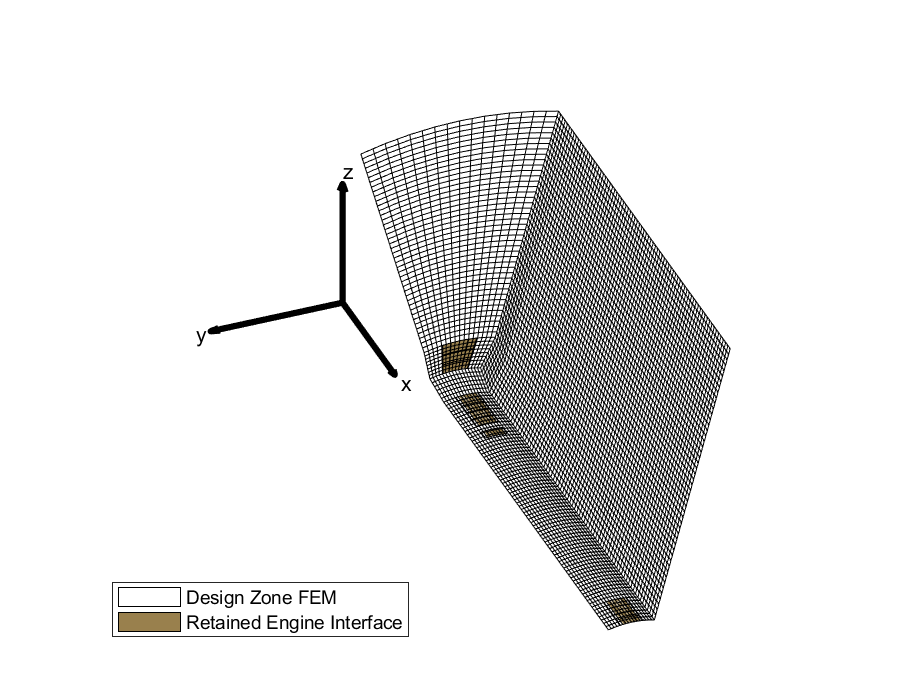
\includegraphics[width=0.5\textwidth]{images/Ch2/mesh_ref1.eps}
       }
       \caption{Mesh refinement procedure needed for multi-grid approach for the evaluation of $\left[H\right]$, the engine reduced element set are colored in yellow. Each node of these elements is kept in the engine super element.(a) Original design zone mesh, generated in Abaqus and imported in Matlab by input file parsing. The mesh counts 7600 8-node linear 3D solid finite elements and 9126 nodes. (b) Design zone mesh after refinement. Each element of the original element is cut in 8 new elements, that give a total of 7600$\times$8=60800 8-node linear 3D solid finite elements and  66759 nodes. }
       \label{f.7}
     \end{figure}
 Let's consider two coarser mesh elements and their partition as considered in figure \ref{f.8} whose centroid distance is known $\|\vec{AC}\|$. The minimal distance between centroids of the corresponding finer mesh elements ,$\|\vec{BD}\|$ can be related to $\|\vec{AC}\|$ as :
  \begin{equation}
  \label{e.12}
  \|\vec{AC}\|\leq\|\vec{AB}\|+\|\vec{BD}\|+|\vec{CD}\|
  \end{equation}
 So that:
  \begin{equation}
  \label{e.13}
  \|\vec{BD}\|\geq \|\vec{AC}\|-\|\vec{AB}\|-|\vec{CD}\|
  \end{equation}
  The distances $\|\vec{AB}\|$ and $|\vec{CD}\|$ are also bounded by the radius of the smallest sphere circumscribed around the biggest coarser mesh element $r_{c}$. Therefore equation (\ref{e.13}) becomes:
    \begin{figure}[hbt!]
    \centering
    \subfloat[  \label{f.7a}]{%
             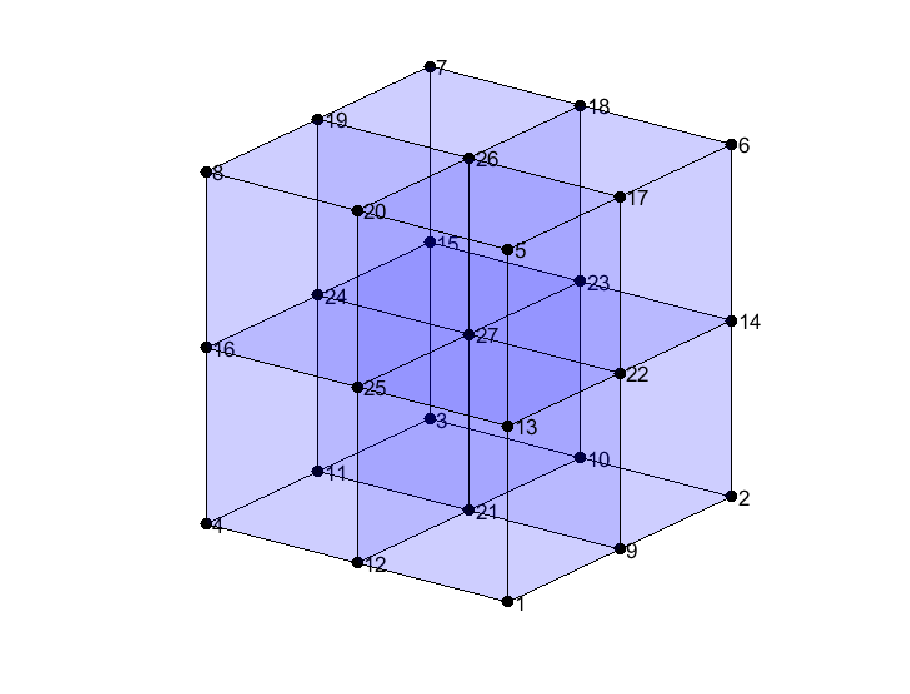
\includegraphics[width=0.5\textwidth]{images/Ch1/partition_3D.eps}
          }
    \subfloat[  \label{f.8}]{
    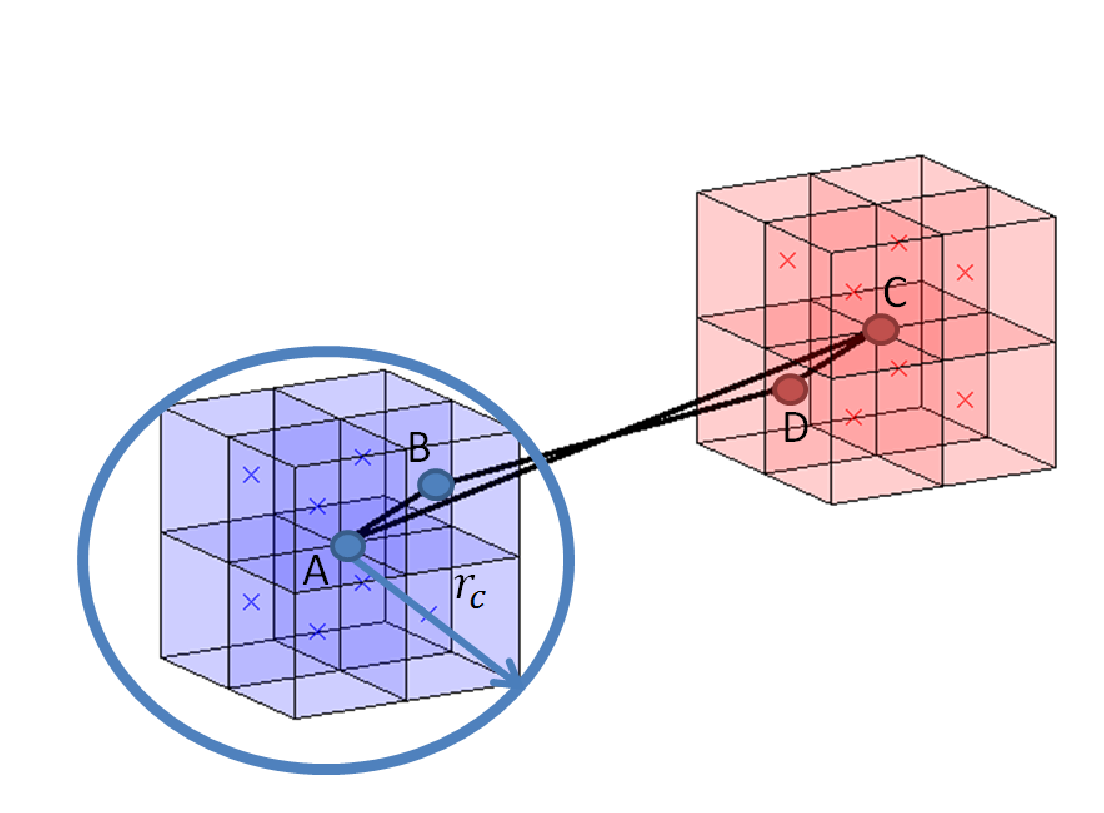
\includegraphics[width=0.5\textwidth]{images/Ch2/minimal_distance.eps}
     }
    \caption{Relation between coarse and fine mesh.
    (a) 3D partition employed for mesh refinement, nodes 1 to 8 belong to the original coarse mesh element. Partition determines node 9 to 27 and 8 elements of the finer mesh.  (b) Scheme of two elements of the original mesh after partition. The relationship between the minimal distance between two finite element centroids in the finer mesh $\|\vec{BD}\|$, the corresponding distance between the centroids of the coarse mesh $\|\vec{AC}\|$ and the radius of the sphere circumscribed around the biggest coarse mesh finite element $r_c$ can be determined considering the vector chain $\vec{AC}=\vec{AB}+\vec{BD}+\vec{DC}$.} 
    \end{figure}
 \begin{equation}
  \label{e.14}
  \|\vec{BD}\|\geq \|\vec{AC}\|-2r_{c}
  \end{equation}
  Note that even if the scheme of figure \ref{f.8} considers cubic elements equation \ref{e.14} is valid for general 8-node brick elements.
  If the distances between coarse mesh centroids are known, it is possible to set-up a test on these distances that can help to reduce the number of centroid-to-centroid distances that have to be computed for the finer mesh.
  In fact for equation \ref{e.14}:
   \begin{equation}
    \label{e.15}
     \|\vec{AC}\|\geq 2r_{c}+r \Rightarrow\| \vec{BD}\|\geq r
    \end{equation}
   Then the distance that for sure needs not to be computed in the finer mesh are the one between elements obtained from coarser mesh at a distance greater than $2r_{c}+r$. On the other hand we cannot conclude that each and every distance that one can evaluate in this way will be smaller than $r$. The final cost of $\left[H\right]$ is then equal to $28N_c+64N_c^*$ where $N_c$ is the number of elements in the coarse mesh and $N_c^*$ is the number of coarse mesh element pairs at a distance less or equal to $ 2r_{c}+r$. Since $N_c=\frac{N_{el}}{8}$ and for reasonably small $r$, $N_c^*=KN_c \ll (N_c)^2$ the cost for this procedure grows up with $(\frac{7}{4}+8K)N_{el}$, linearly and not quadratically with the problem size $N_{el}$. One can note that this procedure is also suitable for parallel implementations, thus further decreasing its numerical cost.
   \newpage
 \subsection{2D topology optimization examples}
In this section we present the implementation of 2D structural topology optimization of structure supposed to be in plane stress. The implementation stems from the very well-known 88 lines Matlab code \cite{andreassen2011efficient}, that here has been implemented with some modifications:
\begin{itemize}
\item The plots have been changed to include load and boundary condition application as the convergence history of compliance and volume fraction. 
\item The test cases considered are the MBB beam, the Short cantilever beam and the L-shape design. The next section will only consider L-shape topology optimization, the other case are in appendix \ref{examples_to2D}.
\item Heaviside filter \cite{guest2004achieving,lazarov2011filters}, penalty \cite{allaire1993numerical,allaire1993topology}, and filter radius \cite{sigmund1997design,sigmund1997designb} continuation were implemented to enforce the solution toward improved local optima with smaller gray regions.
In particular SIMP penalty was increased from 1 to 6, increasing the value of the penalty of 1 each 75 iterations or when the convergence is attained.
Similarly the $\beta$ parameter of the Heaviside filter was increased from 1 to 10.  Finally the value of the filter radius was decreased from a starting value to a minimum value of 2 decreasing its value of 1 every 75 iterations or when convergence is attained.
\item The Optimality Criteria solver was replaced by MMA solver.
\end{itemize}
\begin{table}[h!]
                        % table caption is above the table
                        \caption{Parameters for 2D topology optimization }
                        \label{tab:2.1}       % Give a unique label
                        \centering
                        % For LaTeX tables use
                        \begin{tabular}{lll}
                        \hline\noalign{\smallskip}
                        Parameter & symbol & value\\
                        \noalign{\smallskip}\hline\noalign{\smallskip}
           
                        Full material Young modulus & $E_0$ & $1$\\
                        Void material Young modulus & $E_{min}$ & $10^{-9}$ \\
                        Poisson ratio & $\upsilon$ & $0.3$\\
                        Force amplitude & $F$ & $1$\\
                        Asymptotes initialization & asyinit & $0.5$\\
                        Moving limit & move & 0.1\\
                        Filter type & ft & 3\\
                        Volume fraction & $\upsilon$ & 0.3\\
                        Initial guess & $\VectorVar{x_0}$ & $0.3\VectorVar{1}$
                       \\ Stopping criteria change & tol & $10^{-2}$\\
                        Stopping criteria iterations & maxiter& $1000$\\
                        \noalign{\smallskip}\hline
                        \end{tabular}
                        \end{table} 
The parameters selected for the following analysis are presented in table \ref{tab:2.1} \footnote{the value chosen for the Young's modulus are equal to the one considered by default in top88 Matlab code \cite{andreassen2011efficient}.}. The filter type is equal to 3 and this means that Heaviside filter is adopted.
\newpage
\subsubsection{L-shape optimization}
An interesting 2D use-case is the L-shape optimization c.f. figure \ref{fig.2.15}. 
\begin{figure}[ht]
\centering
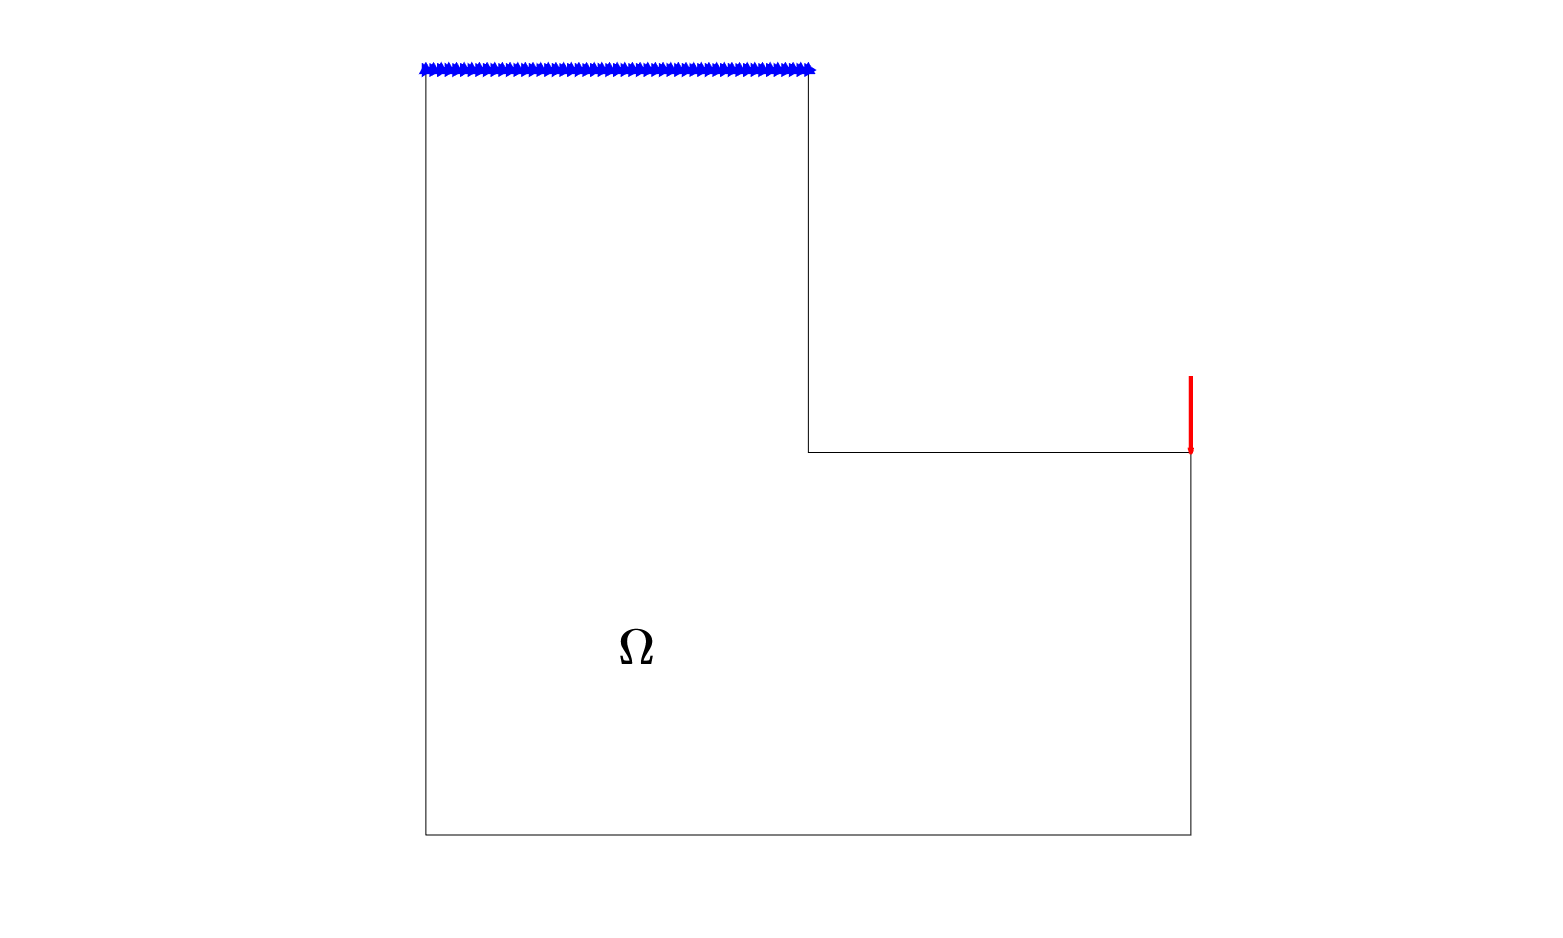
\includegraphics[width=\textwidth]{images/Ch2/design_problem3}
\caption{Geometry, Load and boundary conditions of the L-shape topology optimization problem. Blue triangles are oriented as the fixed DOFs. The red arrows represent the applied loads.}
\label{fig.2.15}
\end{figure}
From an implementation point of view this can be treated with the same top88 framework simply including passive elements. Another important reason that makes this use-case particularly interesting is the fact that the geometry includes at the inner corner a point of stress singularity  in linear elasticity. For this reason it will be worth to mention this use-case again when speaking about stress based topology optimization. Here we proposed to study 2 discretizations: a $50\times50$ and a $100\times100$ mesh.
The initial value of the filter radius was set for the first mesh equal to 4 and for the second mesh equal to 8 (here we recall that the element side length is always 1 in this case). The results are shown in figure \ref{fig.2.16}. A first important observation is that results are not similar. In fact in the design obtained for the coarser mesh we can identify 13 thin members against 11 for the solution found by the refined mesh. This is due to the fact that even using continuation and density filters, the optimization problem still is far from being convex. For this reason finding different local minima is always possible. On the other hand both designs are nearly black and white, both are converged within the maximum iteration number. Selecting the design with the smallest number of members for ease of realization one can still be prone to refuse such design. In fact it is clear that both these designs will have very high stresses in the inner corner and will not be able to bear the load applied to the structure without encountering at least local plasticity, or even failure. In this case we can say that the model is no longer valid for the solution proposed, and that the formulation cannot be considered as acceptable for such a problem. 
\begin{figure}[hbt!]
  \centering
       \subfloat[ \label{fig.2.16a}]{%
                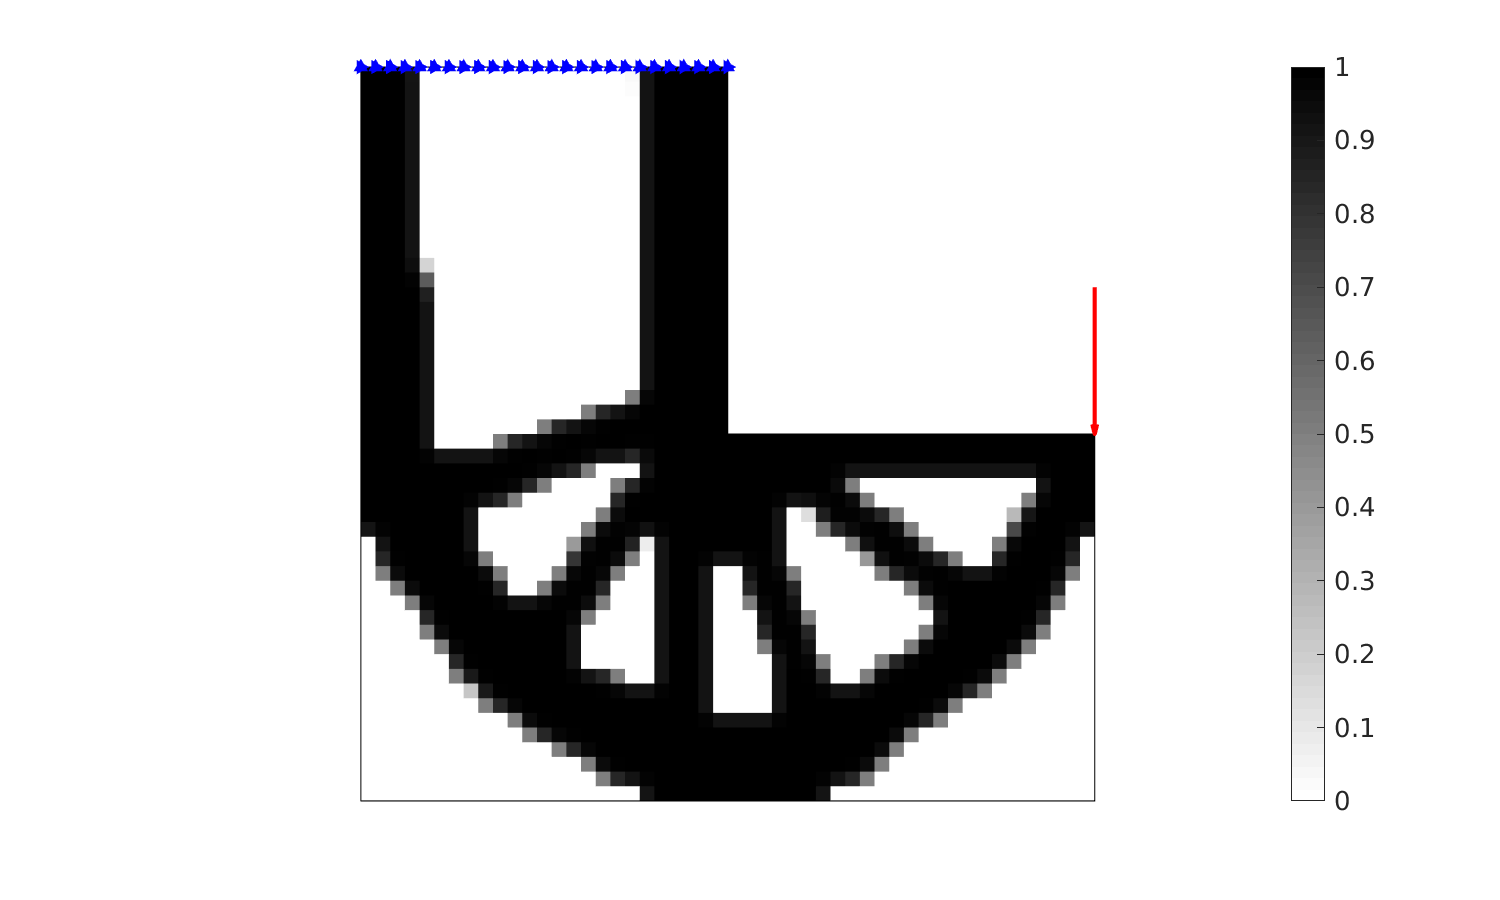
\includegraphics[width=0.5\textwidth]{images/Ch2/L-shapenelx_50nely_50_R_4_volfrac_40_ft_3density}
              }
       \subfloat[  \label{fig.2.16b}]{%
         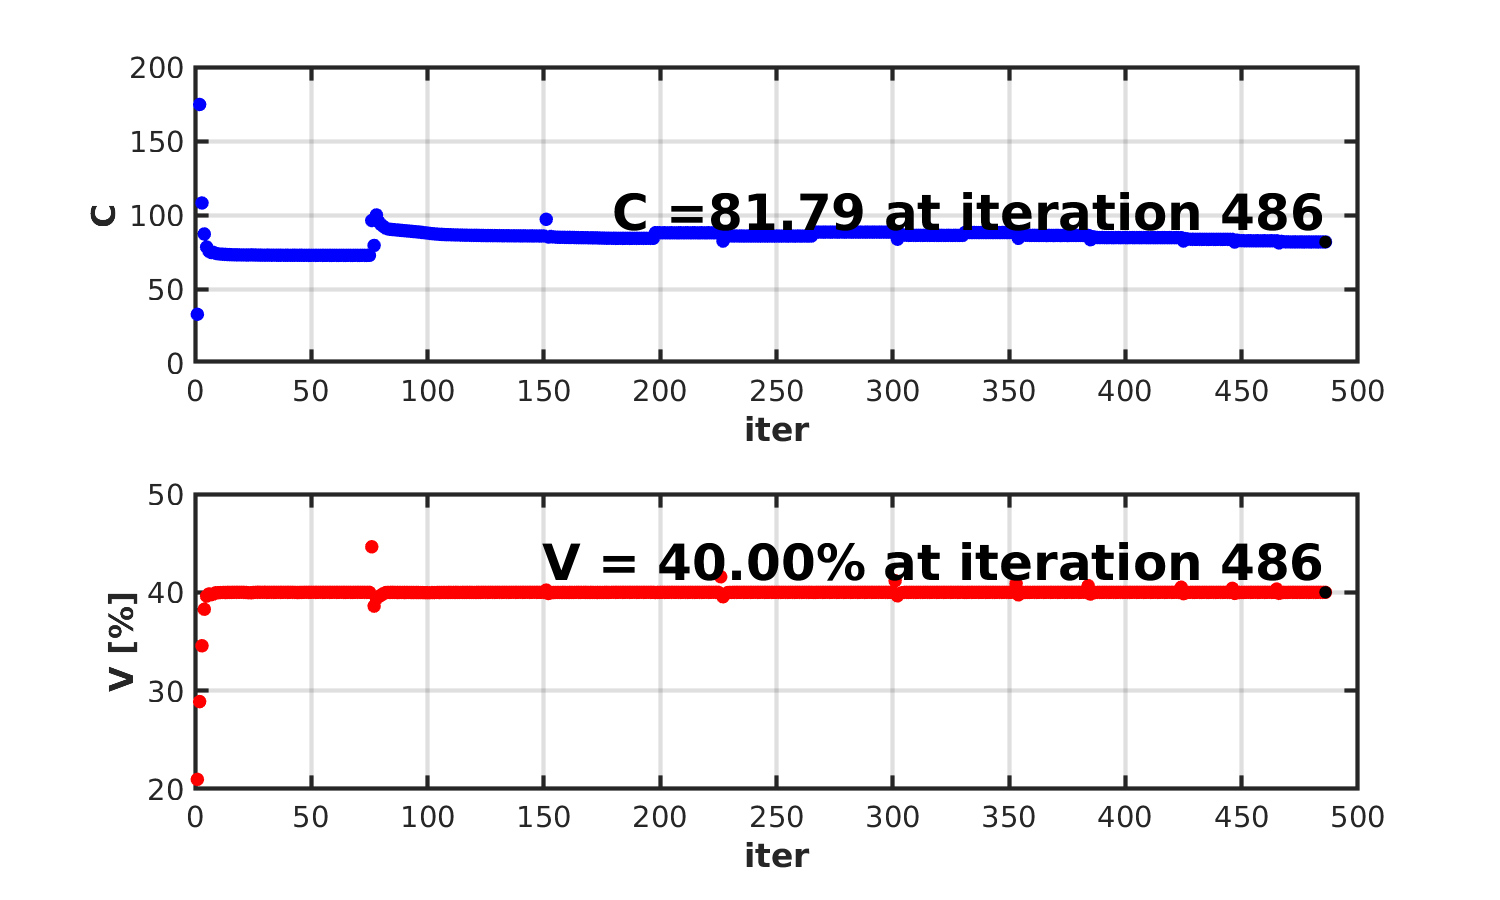
\includegraphics[width=0.5\textwidth]{images/Ch2/L-shapenelx_50nely_50_R_4_volfrac_40_ft_3convergence}
       }
       \\
       \subfloat[ \label{fig.2.16c}]{%
                       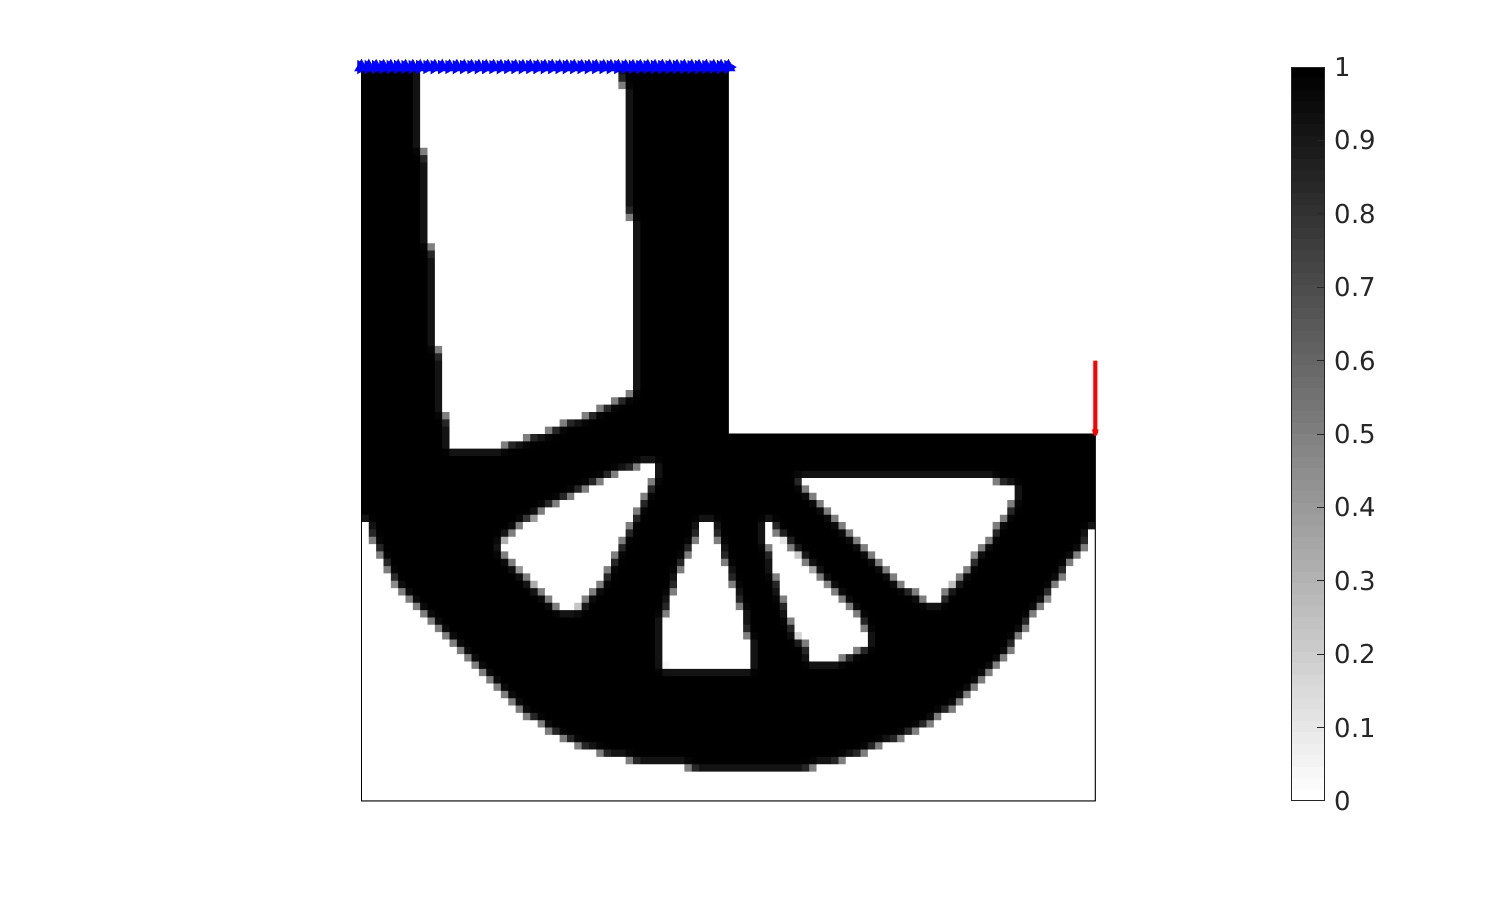
\includegraphics[width=0.5\textwidth]{images/Ch2/L-shapenelx_100nely_100_R_8_volfrac_40_ft_3density}
                     }
              \subfloat[  \label{fig.2.16d}]{%
                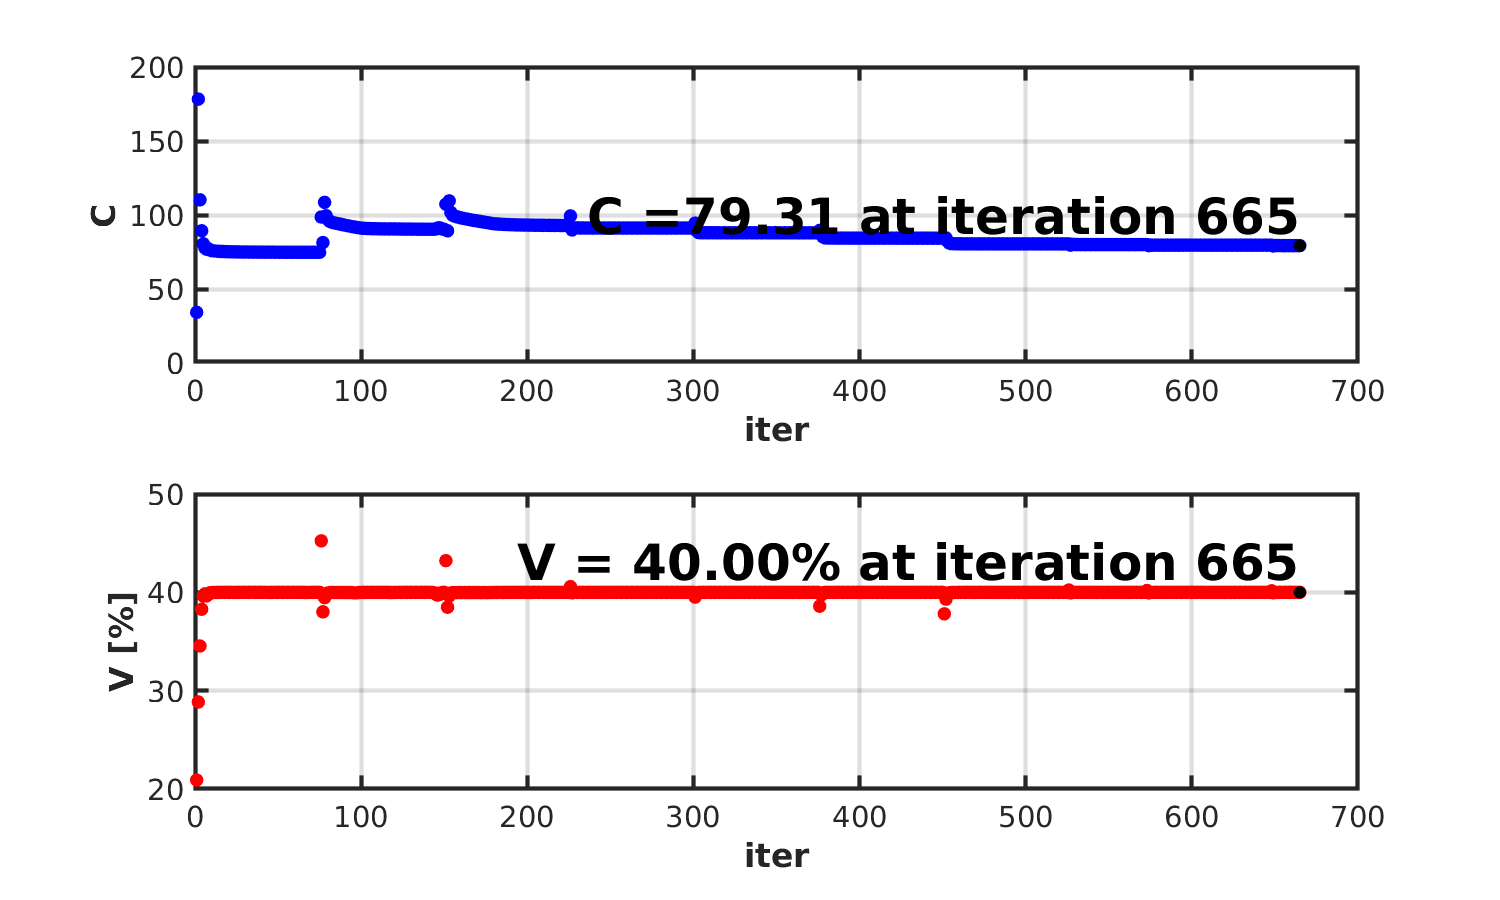
\includegraphics[width=0.5\textwidth]{images/Ch2/L-shapenelx_100nely_100_R_8_volfrac_40_ft_3convergence}
              }
       \caption{L-shape topology optimization results. (a)-(b) $\VectorVar{x_{Phys}}$ distribution and responses convergence for the $50\times 50$ discretization.(c)-(d) $\VectorVar{x_{Phys}}$ distribution and responses convergence for the $100\times 100$ discretization }
       \label{fig.2.16}
     \end{figure}
      \clearpage
\section{Stress based topology optimization}
\label{Sec2.3}
Topology optimization is often related to the minimum compliance problem as it was discussed in the previous section. The problem of this kind of responses is the need of numerous changes that are required in a topology optimization solution to respect failure requirements. For metallic materials a common failure criterion adopted is the von Mises stress that in plane stress can be computed as:
\begin{equation}
\sigma_{VM}=\sqrt{\sigma_{xx}^2+\sigma_{yy}^2-\sigma_{xx}\sigma_{yy}+3\tau_{xy}^2}
\end{equation}
where $\sigma_{xx}$, $\sigma_{yy}$, $\tau_{xy}$ are the corresponding components of the stress tensor. In the FEA they can be computed from the nodal displacements as in equation \eqref{eq.1.40}. In bilinear finite elements like the ones adopted in top88 code, the stresses are not constant over each finite element. If we consider a single query point in the middle of the element matrices $\MatrixVar{D}$ and $\MatrixVar{B}$ of equation \eqref{eq.1.40} becomes:
\begin{eqnarray}
\MatrixVar{B}=\frac{1}{4a}\MatrixVar{\begin{array}{cccccccc}
-1 & 0 & 1 & 0 & 1 & 0 & -1 & 0\\
0 & -1 & 0 & -1 & 0 & 1 & 0 & 1\\
-1 & -1 & -1 & 1 & 1 & 1 & 1 & -1
\end{array}}\\
\MatrixVar{D}=\frac{E}{1-\upsilon^2}\MatrixVar{\begin{array}{ccc}
1 & \upsilon & 0 \\
\upsilon & 1 & 0 \\
0 & 0 & \frac{1-\upsilon}{2}
\end{array}}
\end{eqnarray}
where $2a$ is the mesh side length. For the top88 framework $a=\frac{1}{2}$.  
In figure \ref{fig.2.17} the von Mises stress was shown in each finite element of the solution of figure \ref{fig.2.16c}. 
\begin{figure}[ht]
\centering
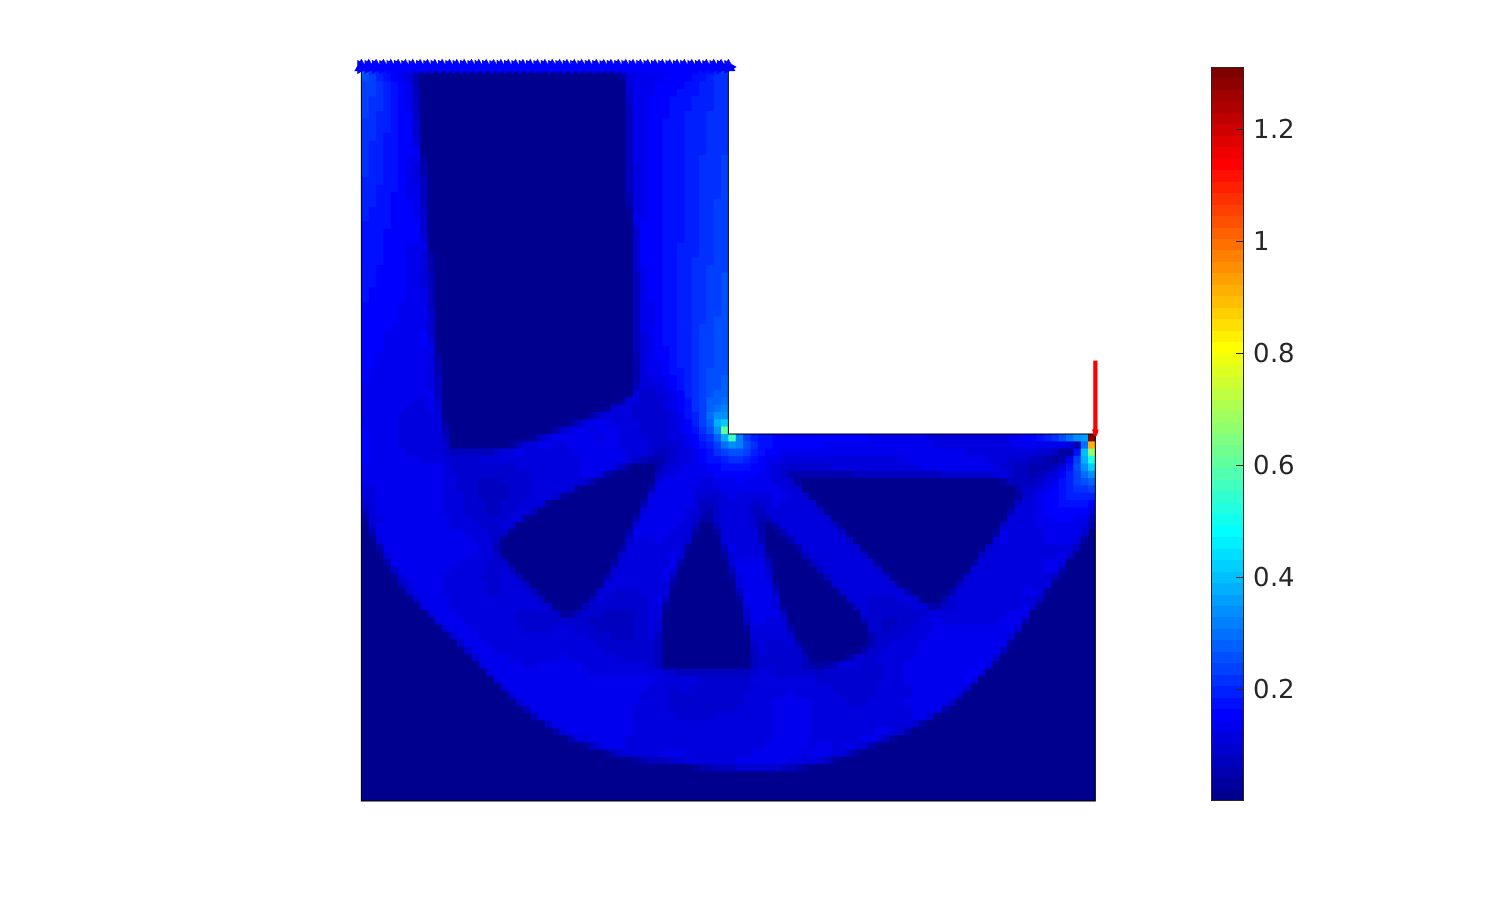
\includegraphics[width=0.9\textwidth]{images/Ch2/L-shapenelx_100nely_100_R_8_volfrac_40_ft_3VM_stress}
\caption{von Mises stress map for the solution of the L-shape optimization for the $100\times100$ mesh.}
\label{fig.2.17}
\end{figure}
As aforementioned 2 stress singularities can be found in both the load application region and in the L-shape inner corner. 
The first depends on the stress model applicability when loads are modeled as nodal forces. This singularity can be eliminated simply changing the modeling hypothesis and considering a distributed load instead. The second is an actual singularity. In fact in the inner corner local plasticity will be attained if the design is manufactured as the solution. To avoid such issues, a fillet should be considered and the solution should therefore be modified. 
Moreover we can say that the problem formulation \ref{compl_formulation} doesn't enforce the solution to respect any allowable limit on the von Mises.
Including stress constraints directly inside the design loop is therefore useful because it can help reducing the gap between optimized and final design. Instead of focusing on the stiffest design respecting some mass requirement, it is often more reasonable to think about the lightest design that fulfills all failure criteria i.e.:
\begin{equation}
\label{formulation_stress}
\begin{cases}
\min_{\VectorVar{0}\leq\VectorVar{x}\leq\VectorVar{1}} {\VectorVar{|\Omega_{el}|}^T\VectorVar{x}} \\
\textit{s.t.}\\
\left(\sigma_{VM}\right)_i\leq \sigma_{lim} & \forall i|x_i>0
\end{cases}
\end{equation}
On the other hand several difficulties arise when including such responses in the optimization formulation. 
In this section we discuss stress based topology optimization and the challenges that need to be addressed due to the nature of stress constraints.
Two major challenges arise in the implementation of stress constraints: the fact that the optimization problem presents singular optima \cite{kirsch1990singular,cheng1997varepsilon,rozvany2001design}, and the large number of stress constraints to be considered.
The first issue consists in the fact that local optima belong to degenerate subspaces of the feasible domain that are not reachable using standard gradient-based optimizations.  The second issue consists in the fact that stress constraints are local, i.e. the stress should be controlled in every point of the structure. Theoretically an infinity of constraints should therefore be considered in the optimization formulation. Instead the stress is limited only in each finite element Gauss point (where the stress recovered by finite element method is the most accurate \cite{zlamal1978superconvergence,zhang2006natural}). Still the number of constraints to be considered is very high and most optimizers available have very hard time dealing with so many local constraints.
One way of dealing with singular optima consists in relaxing stress constraints (for instance using $\epsilon$-relaxation \cite{cheng1997varepsilon}, or the q-p approach \cite{bruggi2008alternative}). To avoid the consideration of many local constraints to the optimization formulation a global constraint can be considered instead, using the maximum function.  To avoid derivation difficulties, regular approximation of the maximum function (for instance the Kreisselmeier-Steinhauser
function \cite{kreisselmeier1980systematic,yang1996stress} or the p-norm \cite{duysinx1998new} ) can be considered. Aggregation techniques have the main drawbacks of not having a precise control on the final design maximum stress. To control the exact value of maximum stress in the final solution Le et al. \cite{le2010stress} proposed an adaptive approach that helps obtaining designs with the desired maximum stress.  In this work we adopted the formulation presented in \cite{verbart2017unified}.
In this approach each finite element is considered as a composite containing both full material and voids. The collapse in the structure is considered attained when the stress inside the full material reaches the allowable. For this reason one has to describe the microscopic stress inside a finite element as:
\begin{equation}
\hat{\sigma}_{VM}=\frac{E_0\sigma_{VM}}{E}
\end{equation}
In this way the stress computed in element that have densities approaching zero, will tend to a finite value and not to 0. Then the relaxed constraint violations can be defined for each Gauss point in each finite element as:
\begin{equation}
\label{eq.2.30}
\bar{g_i}=(x_{Phys})_i\left(\frac{(\hat{\sigma}_{VM})_i}{\sigma_{lim}}-1\right) \quad \forall i=1,2,...,N_{GP}
\end{equation}
where $(x_{Phys})_i$ is the physical density corresponding to the element including the $i^{th}$ Gauss point.
These violations are positive when the microscopic stresses are greater than the allowable but are equal to 0 when an element has zero density. In this way it is proven that singular optima can be attained by gradient based solver.
The aggregated stress is finally evaluated by the use of the lower bound Kreisselmeier-Steinhauser
function \cite{kreisselmeier1980systematic} that approximates the local relaxed stress constraint violation maximum:
\begin{equation}
\label{e.KSl}
G^{l}_{KS}=\frac{1}{P}\ln\left(\frac{1}{N_G}\sum_{i=1}^{N_G}e^{P\bar{g}_i}\right)
\end{equation}
where $N_G$  is the total number of Gauss point and $P>1$ is the aggregation constant. When evaluating equation \eqref{e.KSl} on design that violating the stress constraint, very large numbers are summed together with smaller numbers. This can lead to have a numerical infinity to be attained by the KS function due to the machine representation limitation.
To avoid such numerical issues, the formulation of equation \eqref{e.KSl} can be rewritten as:
\begin{equation}
\label{eq.2.32}
G^{l}_{KS}=\bar{g}_{max}+\frac{1}{P}\ln\left(\sum_{i=1}^{N_G}e^{P\left(\bar{g}_i-\bar{g}_{max}\right)}\right)-\frac{\ln\left(N_G\right)}{P}
\end{equation}
Where $\bar{g}_{max}=\max_i\bar{g}_i$. We provide in Appendix \ref{Appendix1} some useful properties of the $G_{KS}^l$ function and that equation \eqref{eq.2.32} and \eqref{e.KSl} are equivalent. The reader can observe that equation \eqref{eq.2.32} is differentiable and its derivatives is given by differentiation of equation \eqref{e.KSl} that is provided later in this section. 
The satisfaction of stress constraints is thus imposed in problem (\ref{formulation_stress}) as:
\begin{equation}
\begin{cases}
\label{Verbart_formulation}
\min_{\VectorVar{0}\leq\VectorVar{x}\leq\VectorVar{1}} {\VectorVar{|\Omega_{el}|}^T\VectorVar{x}} \\
\textit{s.t.}\\
G^{l}_{KS}\leq 0 
\end{cases}
\end{equation}
The reader can observe that this is only one of the possible ways of aggregating constraints available in literature.  One can also use P-mean \cite{duysinx1998new} or Induced Exponential \cite{kennedy2015improved} approximation of maximum. In chapter 3 we will see these approaches in much deeper details.
A second important observation about formulation \ref{Verbart_formulation} is that $G^{l}_{KS}$ need adjoint evaluation of sensitivities. Here we propose a short computation chain for the partial derivatives $\VectorVar{\frac{\partial G_{KS}^l}{\partial x_{Phys}}}$ and  $\VectorVar{\frac{\partial G_{KS}^l}{\partial U}}$:
\begin{eqnarray}
\VectorVar{\frac{\partial G_{KS}^l}{\partial x_{Phys}}}^T=\VectorVar{\frac{\partial G_{KS}^l}{\partial \bar{g}}}^T\MatrixVar{\frac{\partial  \bar{g}}{\partial x_{Phys}}}\\
\VectorVar{\frac{\partial G_{KS}^l}{\partial U}}^T=\VectorVar{\frac{\partial G_{KS}^l}{\partial \bar{g}}}^T\MatrixVar{\frac{\partial  \bar{g}}{\partial U}}
\end{eqnarray}
where:
\begin{eqnarray}
\label{eq.2.64}
\frac{\partial G_{KS}^l}{\partial \bar{g}_i}=\frac{e^{P\bar{g}_i}}{\sum_{j=1}^{N_G}e^{P\bar{g}_j}} \\
\frac{\partial  \bar{g}_i}{\partial x_j}=\delta_{ij} \left(\frac{(\hat{\sigma}_{VM})_i}{\sigma_{lim}}-1\right)\\
\frac{\partial  \bar{g}_i}{\partial U_j}=\frac{(x_{Phys})_i}{\sigma_{lim}}\frac{\partial (\hat{\sigma}_{VM})_i} {\partial U_j}\\
\delta_{ij}=\begin{cases}
1 & \textit{if } i\in GP_j \\
0 & \textit{otherwise.}
\end{cases}
\end{eqnarray} 
Where $GP_j$ is the ensemble of j-th element Gauss Point indexes. Numerical issues similar to the one described for the evaluation of equation \eqref{e.KSl} are encountered in the evaluation of equation \eqref{eq.2.64}. Since the numerator and the denominator can be described as an infinite value by the machine a Not a Number (NaN) can be produced from this expression. This is why the following expression (equivalent to \eqref{eq.2.64}) should be employed:
\begin{equation}
\frac{\partial G_{KS}^l}{\partial \bar{g}_i}=\frac{e^{P\left(\bar{g}_i-\bar{g}_{max}\right)}}{\sum_{j=1}^{N_G}e^{P\left(\bar{g}_j-\bar{g}_{max}\right)}} \\
\end{equation}
 For the computation of $\frac{\partial (\hat{\sigma}_{VM})_i} {\partial U_j}$ it is worthy to introduce some simplifications in the expression of $(\hat{\sigma}_{VM})_i$:
\begin{eqnarray}
(\hat{\sigma}_{VM})_i=\sqrt{\VectorVar{\hat{\sigma}_i}^T \MatrixVar{\begin{array}{ccc}
1 & -0.5 & 0\\
-0.5 & 1 & 0\\
0 & 0 & 3
\end{array}}\VectorVar{\hat{\sigma}_i}}=\sqrt{\VectorVar{U_i}^T \MatrixVar{\hat{S}}\VectorVar{U_i}}\\
\VectorVar{\hat{\sigma}_i}=\VectorVar{\begin{array}{c}
(\hat{\sigma}_{xx})_i\\
(\hat{\sigma}_{yy})_i\\
(\hat{\tau}_{xy})_i
\end{array}}
\end{eqnarray}
Where $\VectorVar{\hat{\sigma}_i}$ is the vector containing the stress components in the $i^{th}$-Gauss point, $\VectorVar{U_i}$ represent the vector of nodal displacement of the element containing the same Gauss point taken in the order of the local DOF sorting. Moreover:
\begin{eqnarray}
\MatrixVar{\hat{S}}=\MatrixVar{B}^T\MatrixVar{\hat{D}}^T\MatrixVar{T}\MatrixVar{\hat{D}}\MatrixVar{B}\\
\MatrixVar{T}=\MatrixVar{\begin{array}{ccc}
1 & -0.5 & 0\\
-0.5 & 1 & 0\\
0 & 0 & 3
\end{array}}\\
\MatrixVar{\hat{D}}=\frac{E_0}{E}\MatrixVar{D}
\end{eqnarray}
where $\MatrixVar{T}$ is a constant matrix. It can be noticed that $\MatrixVar{\hat{D}}$ is a property of the full material and is not function of the physical density.
With all these simplification considered:
\begin{equation}
\frac{\partial (\hat{\sigma}_{VM})_i} {\partial U_j}=\frac{\VectorVar{\frac{\partial \VectorVar{U_i}}{\partial U_j}}^T\MatrixVar{\hat{S}}\VectorVar{U_i} }{(\hat{\sigma}_{VM})_i}
\end{equation}
where $\VectorVar{\frac{\partial \VectorVar{U_i}}{\partial U_j}}$ contains either 1 or 0 if the index j correspond to one of the component of vector $ \VectorVar{U_i}$. 
\subsection{A 2D stress based topology optimization example}
In this section we tested the stress based formulation of eq. \ref{Verbart_formulation} on the L-shape topology optimization problem. The stress based formulation is much more dependent on optimization tuning than the compliance one. To avoid MMA divergence, the optimizer step length (i.e. the distance between a design and the one at the previous iteration) need to be controlled. Several strategies can be adopted for this purpose directly using the MMA Matlab code \cite{svanberg1987method}. One can use the move limit defined by the variable move. This variable controls the lower and upper bound defined in the approximated optimization problem, so that the optimization step length is directly controlled. There is a second way of reducing the optimizer step in a more indirect way. This consists in reducing the maximum distance of asymptotes from the current point. In this way the local approximation adopted for constraints will be violated faster. This implicitly reduces the optimizer step length when the sub-solver iterations converge to a minimum of the local approximation. As suggested by \cite{verbart2017unified} we adopted this second strategy. The domain of interest is $100\times100$. Both the effect of discretization and aggregation was considered.
Continuation strategy was adapted as for the compliance formulation. On the other hand, this time the filter radius was kept constant to the value of 2 mesh size and the beta parameter was increased only up to 6. The increment of $\beta$ and the SIMP penalty were applied every time that convergence was attained or every 300 iterations. The convergence criterion was also on the infinity norm of the variation of design vector. This time a value of 0.001 was selected as convergence tolerance. The maximum of iterations was set to 10000. To avoid modeling issues on the stress the nodal force applied as in figure \ref{fig.2.17} was replaced by a linear force distribution over a length of 5. In table \ref{tab:2.2}\footnote{The values adopted in this study are similar to the one considered in \cite{verbart2017unified}.} the optimization set-up is summarized.
\begin{table}[h!]
                        % table caption is above the table
                        \caption{Parameters for 2D stress based topology optimization}
                        \label{tab:2.2}       % Give a unique label
                        \centering
                        % For LaTeX tables use
                        \begin{tabular}{lll}
                        \hline\noalign{\smallskip}
                        Parameter & symbol & value\\
                        \noalign{\smallskip}\hline\noalign{\smallskip}
           
                        Full material Young modulus & $E_0$ & $1$\\
                        Void material Young modulus & $E_{min}$ & $10^{-9}$ \\
                        Full material allowable stress & $\sigma_{lim}$ & $1$ \\
                        Poisson ratio & $\upsilon$ & $0.3$\\
                        pressure & $p$ & $\frac{1}{5}$\\
                        Asymptotes initialization & asyinit & $0.5$\\
                        Moving limit & move & 0.5\\
                        External Moving limit \cite{verbart2017unified}  &   & 0.1\\
                        Filter type & ft & 3\\
                        Volume fraction & $\upsilon$ & 0.3\\
                        Initial guess & $\VectorVar{x_0}$ & $\VectorVar{1}$
                       \\ Stopping criteria change & tol & $10^{-3}$\\
                        Stopping criteria iterations & maxiter& $10000$\\
                        \noalign{\smallskip}\hline
                        \end{tabular}
                        \end{table} 
The effect of $P$ on the topology optimization is shown in figure \ref{fig.2.18}. A first important remark is that $G_{KS}^l$ is always lower than the actual $\bar{g}_{max}$. As a consequence the maximal von Mises stress is always greater than the actual allowable of 1. Increasing the value of P the final stress is decreased, and this is a consequence of equation \ref{ee20}. On the other hand MMA struggles to converge for increasing value of P as it can be seen on the constraint violation convergence history. Moreover even adopting a continuation strategy it can be observed that the solution presents some region of intermediate densities. Finally for $P=16$ and $P=28$ the sharp inner corner is replaced by a fillet. This a very well established design technique to avoid stress concentration which is also found by the optimization algorithm. To improve the accuracy of the maximum stress control one can increase $P$ but this comes at the cost of a higher stress response non-linearity.
\begin{figure*}[h!]
\centering
\subfloat[Density plot $P=4$\label{fig.2.18a}]{{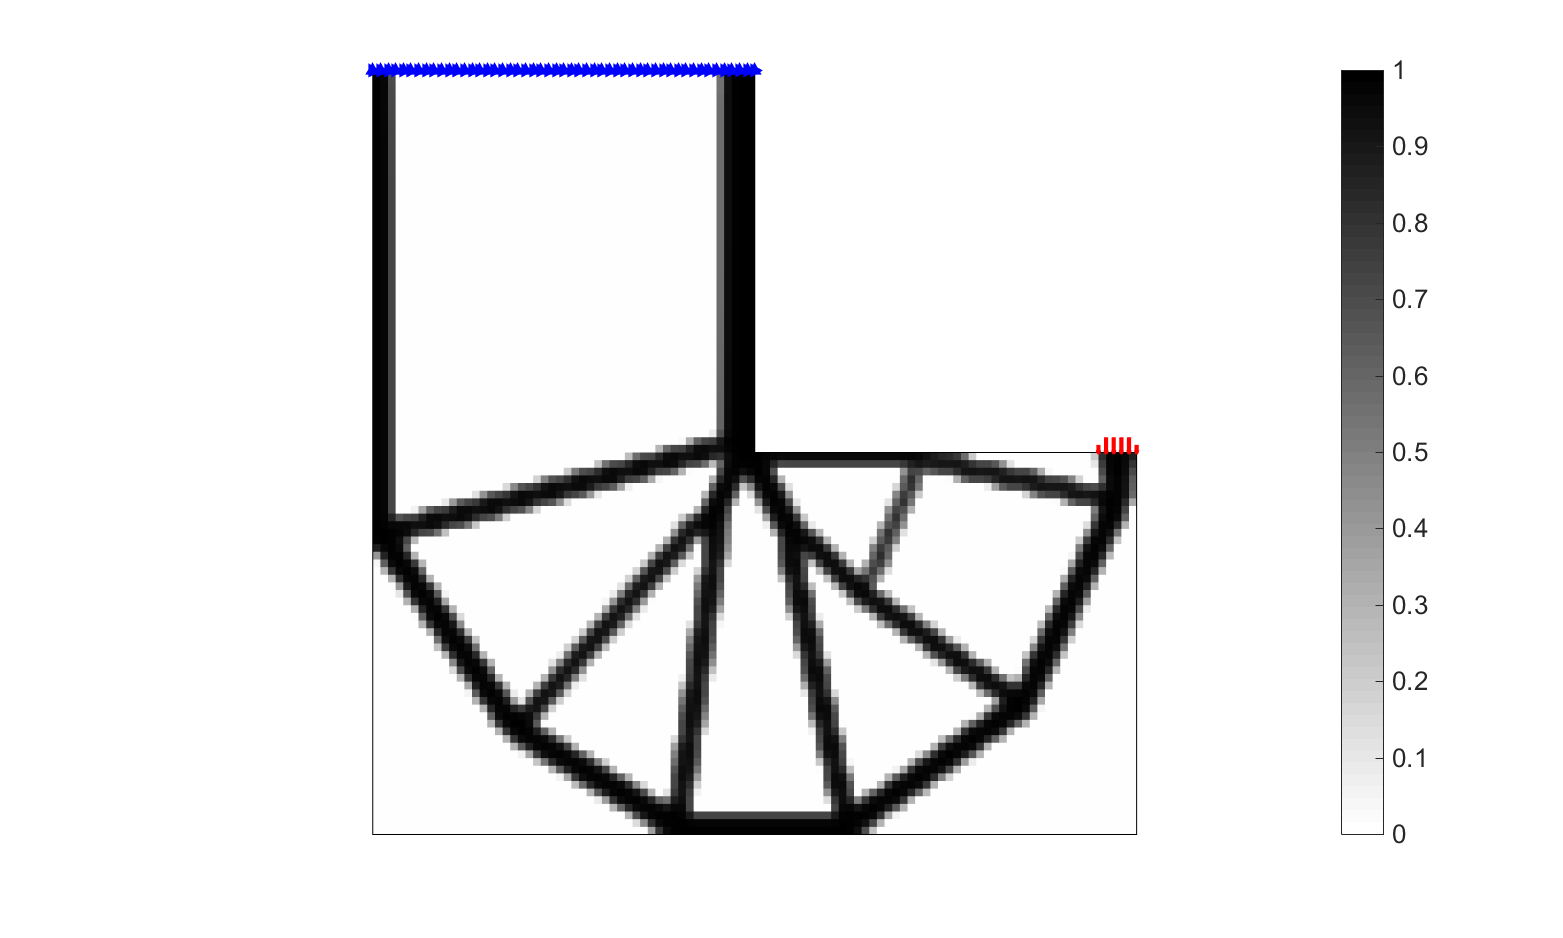
\includegraphics[width=0.45\textwidth]{images/Ch2/L-shapenelx_100nely_100_R_2_P_4_ft_3_Sl_1_KSldensity} }}%
\quad
\subfloat[von Mises plot $P=4$\label{fig.2.18b}]{{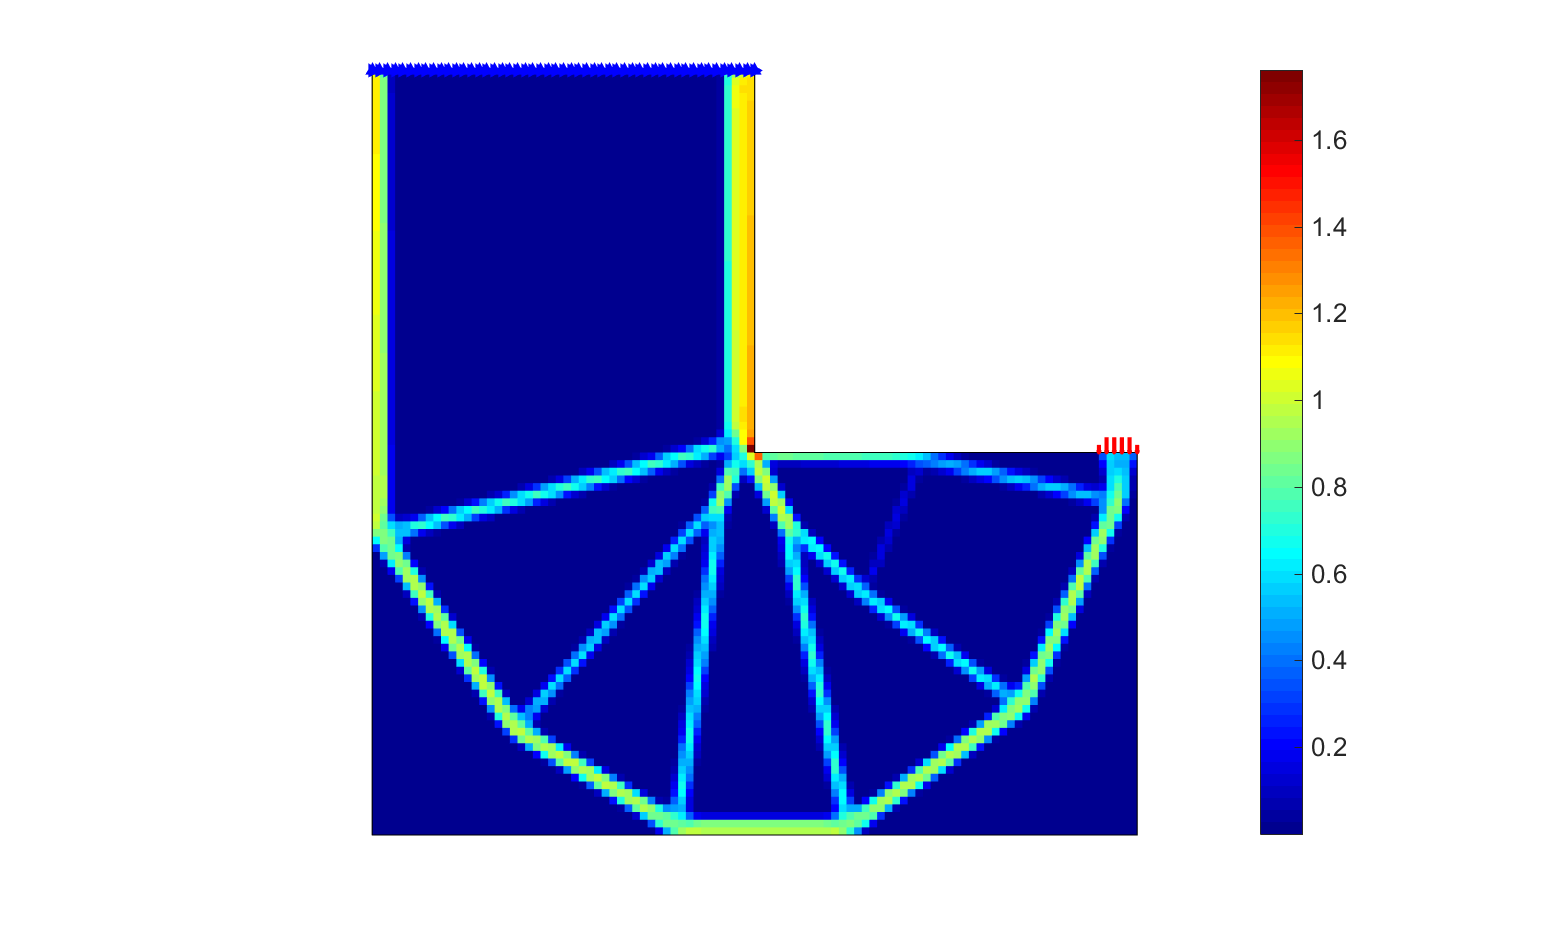
\includegraphics[width=0.45\textwidth]{images/Ch2/L-shapenelx_100nely_100_R_2_P_4_ft_3_Sl_1_KSlVM_stress} }}%
 \\
 \subfloat[Density plot $P=16$\label{fig.2.18d}]{{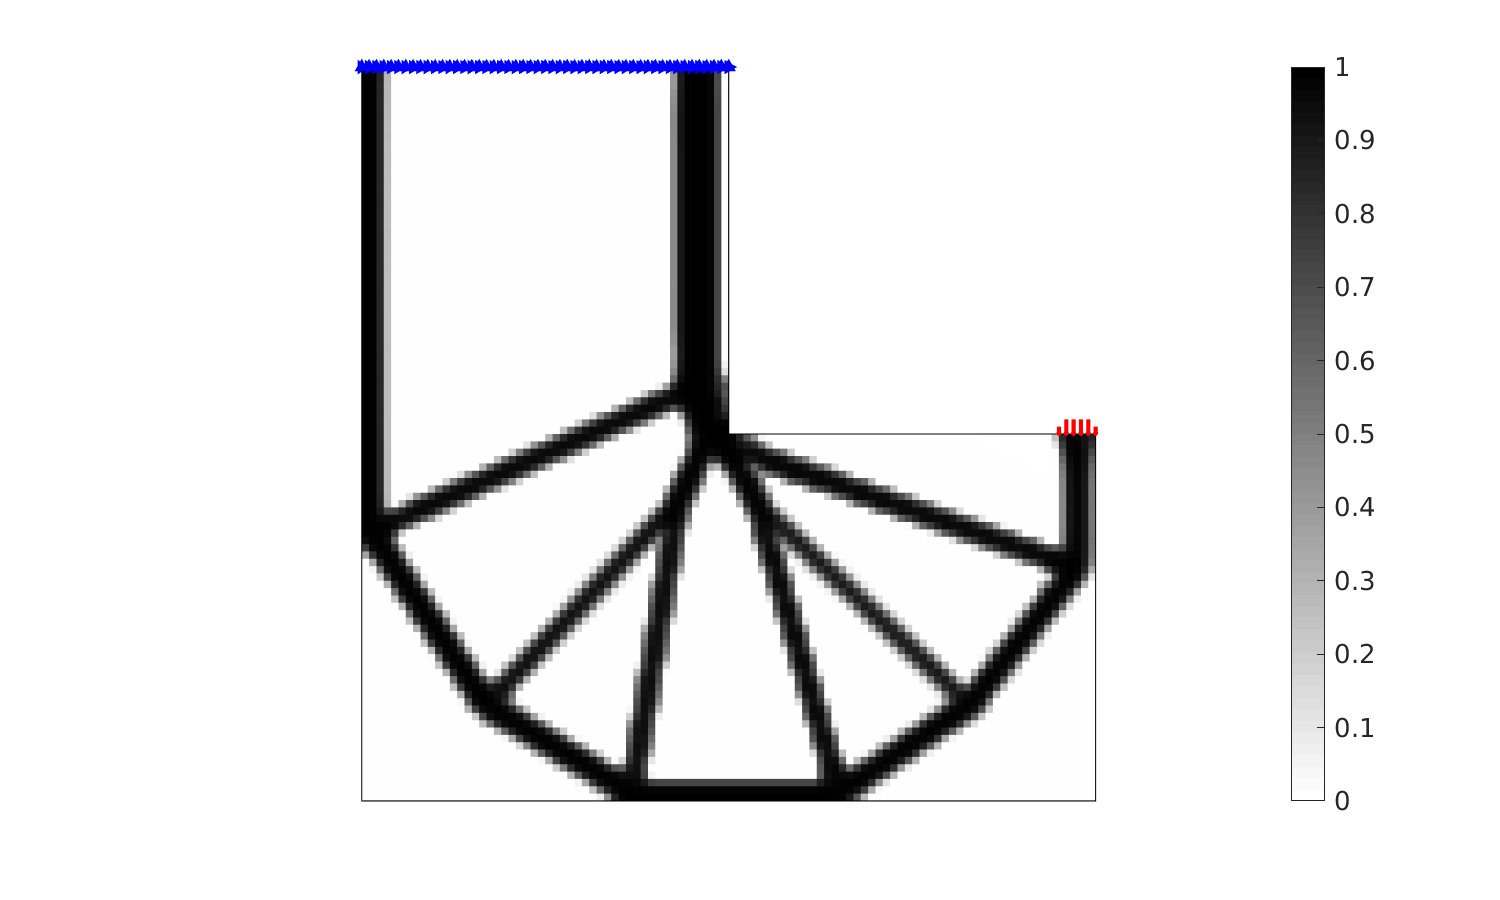
\includegraphics[width=0.45\textwidth]{images/Ch2/L-shapenelx_100nely_100_R_2_P_16_ft_3_Sl_1_KSldensity} }}%
 \quad
 \subfloat[von Mises plot $P=16$\label{fig.2.18e}]{{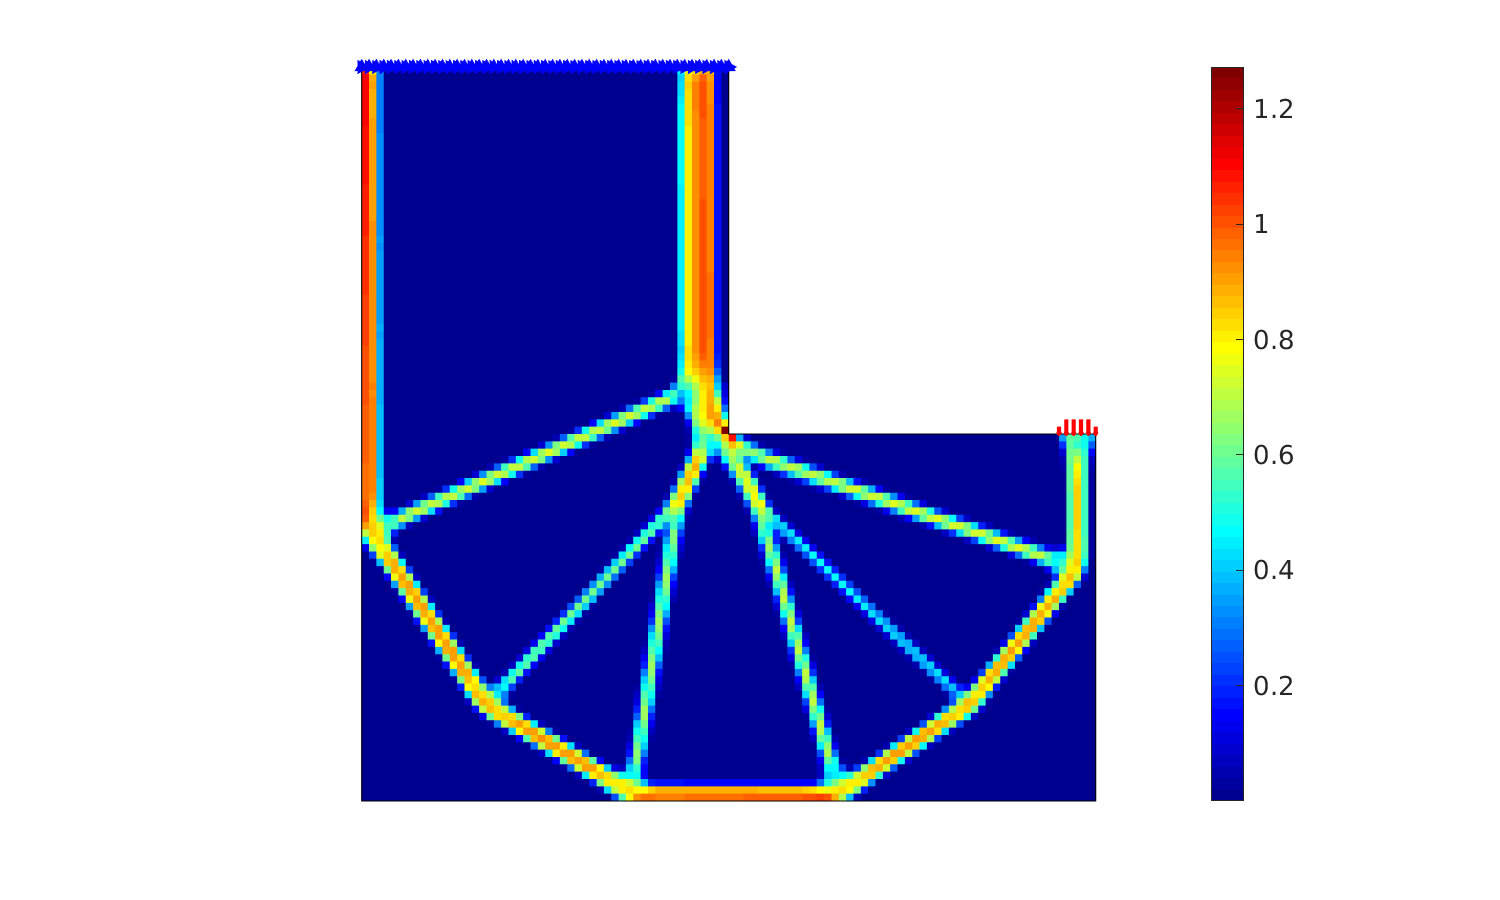
\includegraphics[width=0.45\textwidth]{images/Ch2/L-shapenelx_100nely_100_R_2_P_16_ft_3_Sl_1_KSlVM_stress} }}%
  \\
   \subfloat[Density plot $P=28$\label{fig.2.18g}]{{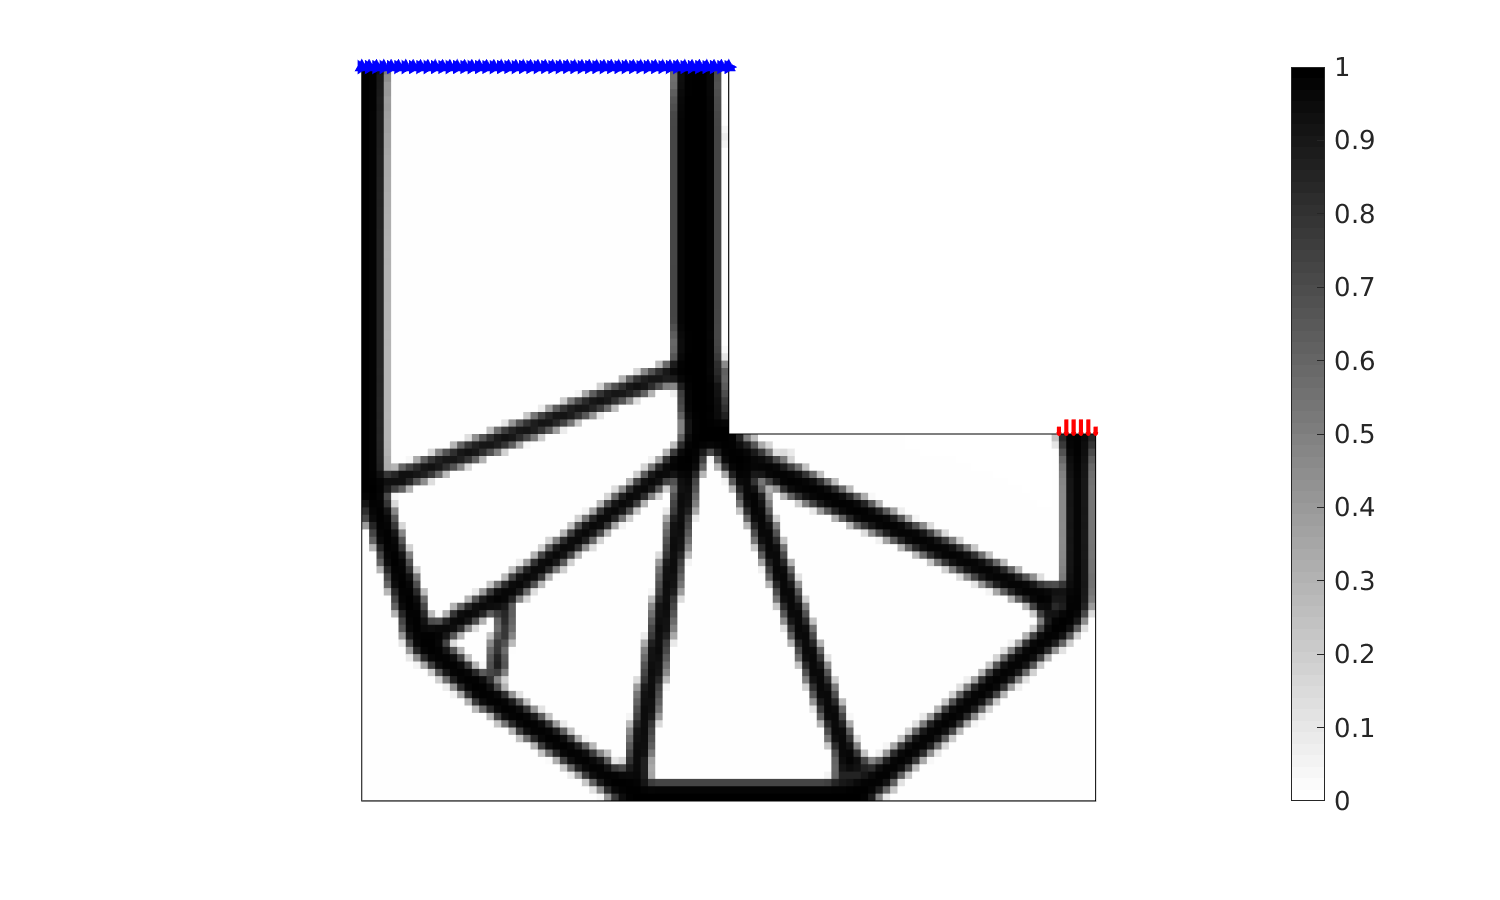
\includegraphics[width=0.45\textwidth]{images/Ch2/L-shapenelx_100nely_100_R_2_P_28_ft_3_Sl_1_KSldensity} }}%
   \quad
   \subfloat[von Mises plot $P=28$\label{fig.2.18h}]{{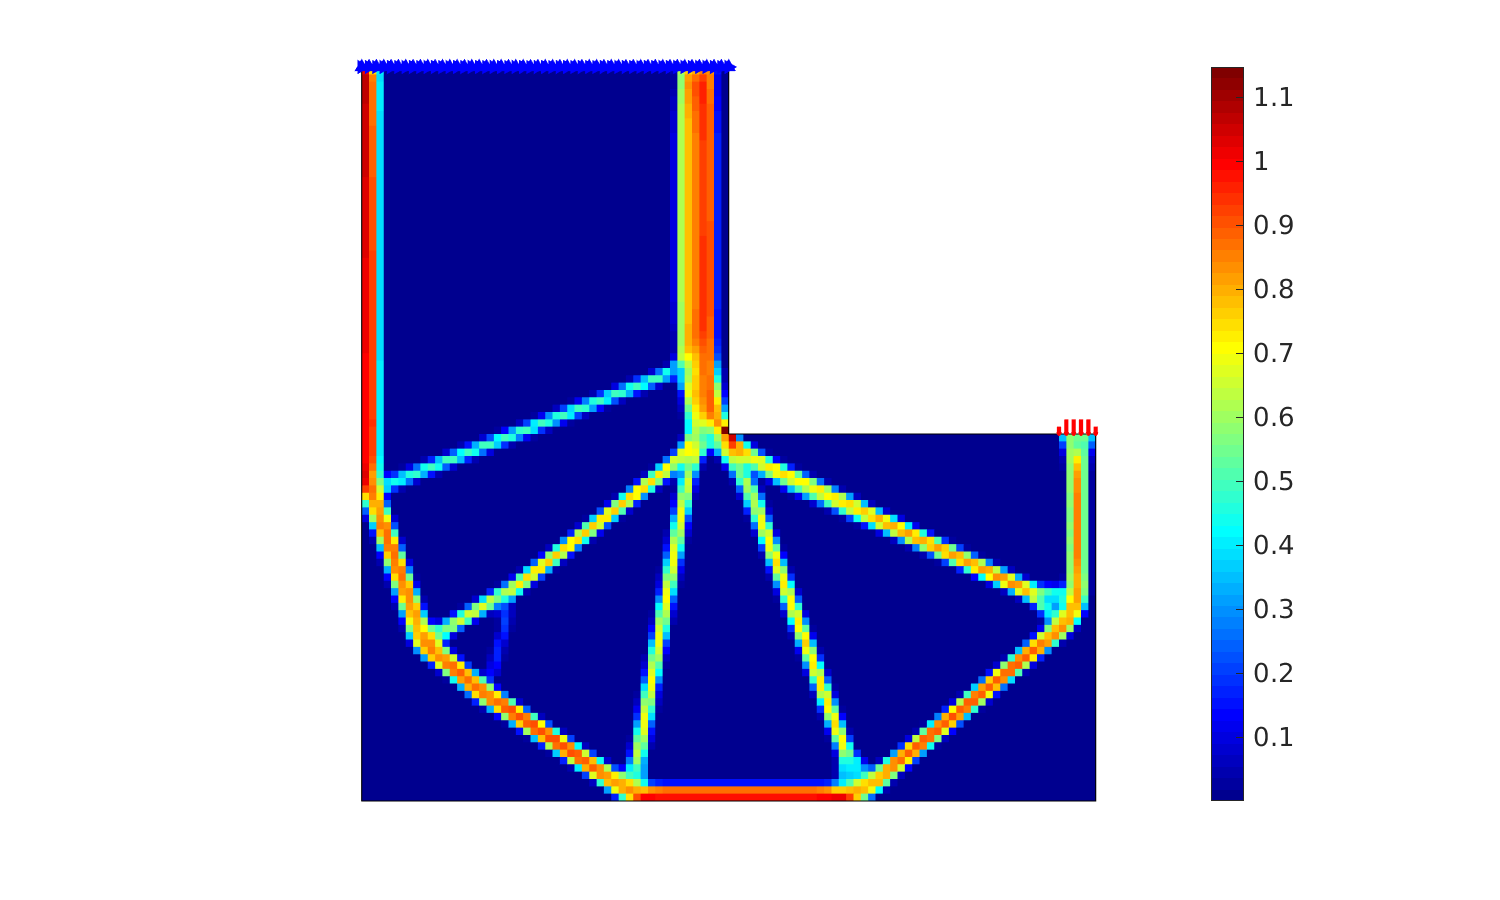
\includegraphics[width=0.45\textwidth]{images/Ch2/L-shapenelx_100nely_100_R_2_P_28_ft_3_Sl_1_KSlVM_stress} }}%     
    \\ 
\caption{L-shape $100\times 100$ mesh resolution, stress based topology optimization results. Density distribution, von Mises stress distribution for $P=4,16,28$ and for $\sigma_{lim}=1$. }%
\label{fig.2.18}%
\end{figure*}
\begin{figure*}[h!]
\centering 
    \subfloat[Convergence plot $P=4$\label{fig.2.18c}]{{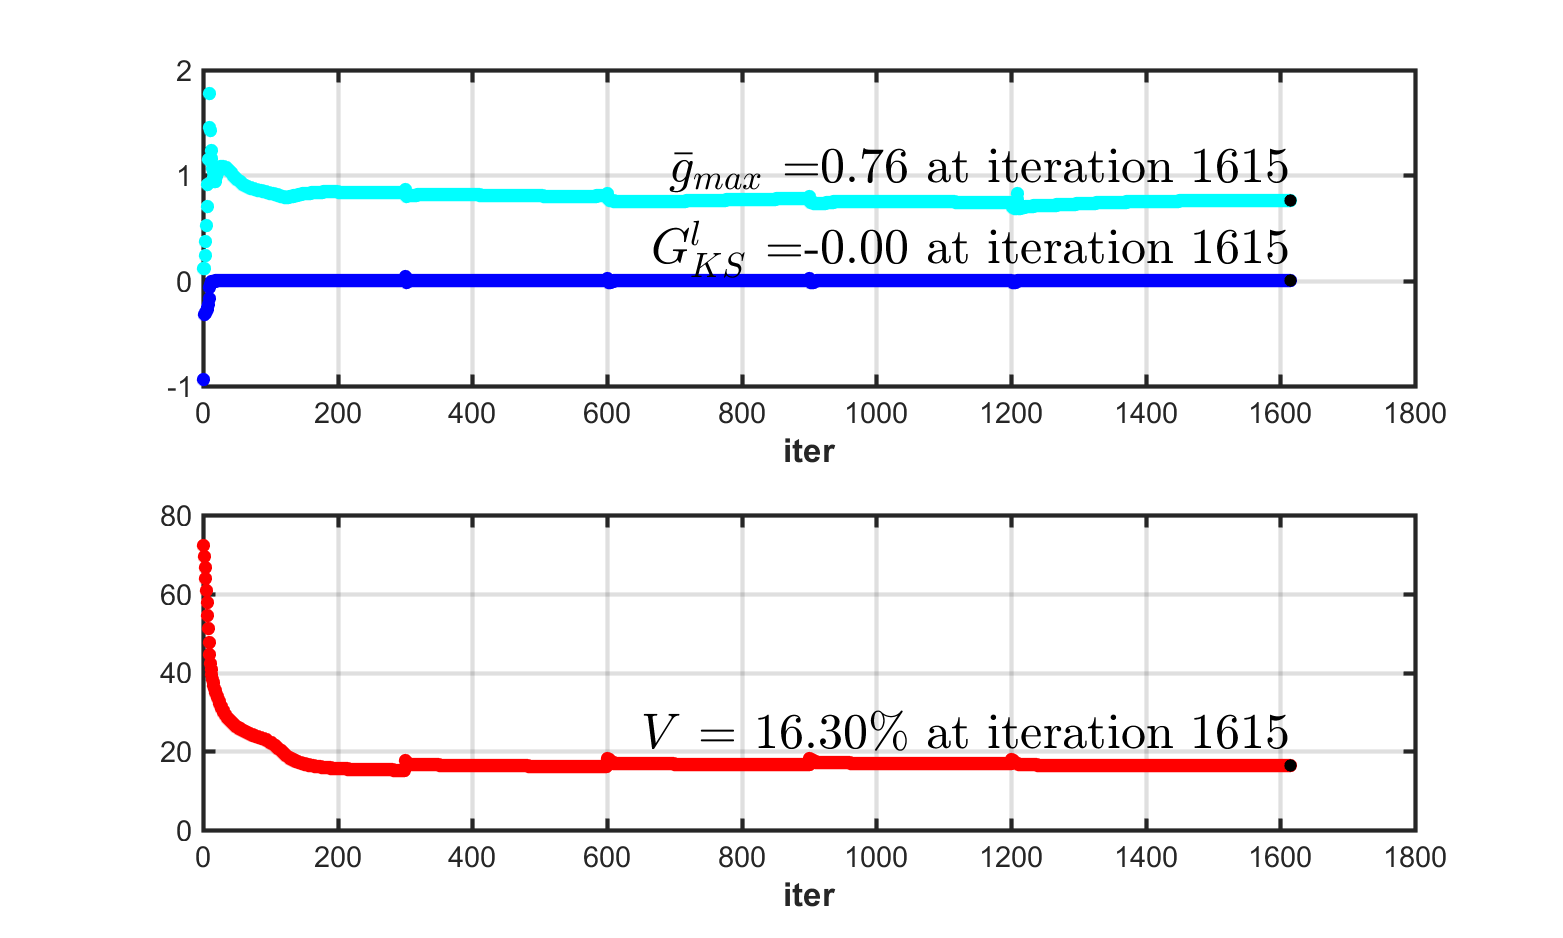
\includegraphics[width=0.6\textwidth]{images/Ch2/L-shapenelx_100nely_100_R_2_P_4_ft_3_Sl_1_KSlconvergence} }}%
 \\
     \subfloat[Convergence plot $P=16$\label{fig.2.18f}]{{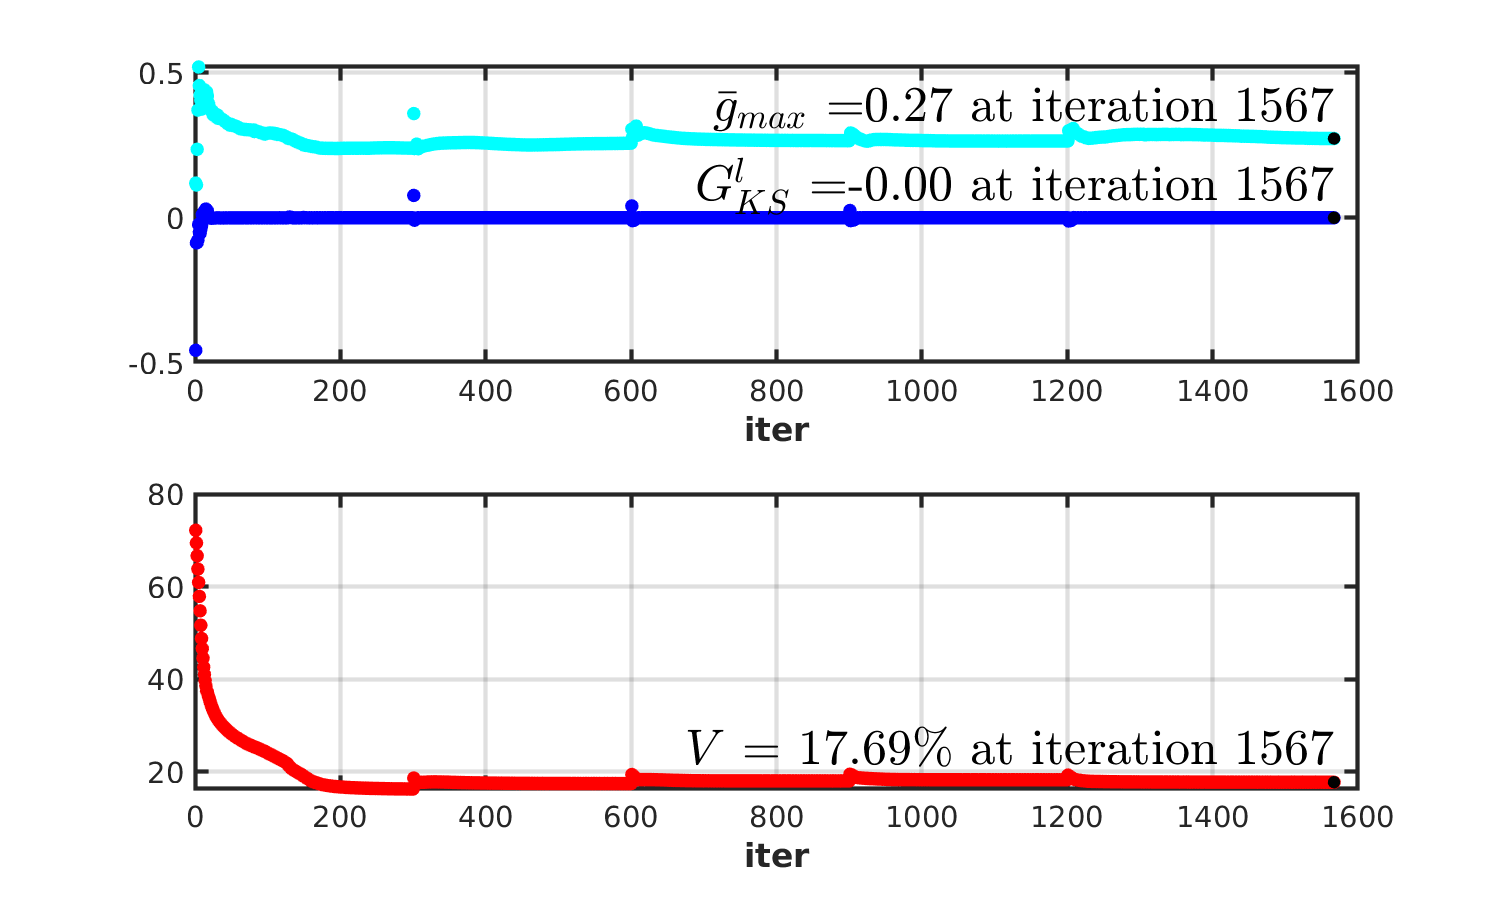
\includegraphics[width=0.6\textwidth]{images/Ch2/L-shapenelx_100nely_100_R_2_P_16_ft_3_Sl_1_KSlconvergence} }}%
  \\
       \subfloat[Convergence plot $P=28$\label{fig.2.18i}]{{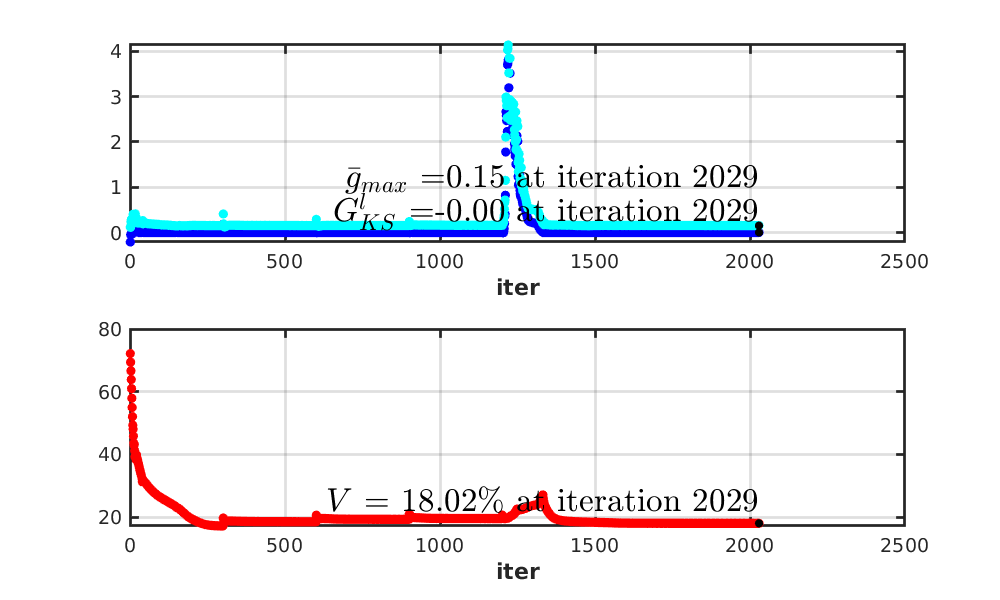
\includegraphics[width=0.6\textwidth]{images/Ch2/L-shapenelx_100nely_100_R_2_P_28_ft_3_Sl_1_KSlconvergence} }}%
\caption{L-shape $100\times 100$ mesh resolution, stress based topology optimization results. Convergence history for $P=4,16,28$ and for $\sigma_{lim}=1$. }%
\label{fig.2.18bb}%
\end{figure*}
In figure \ref{fig.2.19} the effect of $\sigma_{lim}$ is shown for the same mesh discretization. It is interesting to notice that, for $\sigma_{lim}=0.9$ the final stress is actually $\sigma_{max}\approx1.05$ and that for $\sigma_{lim}=0.8$ the final stress becomes $\sigma_{max}\approx0.94$. This suggests the possibility of ensuring the convergence to the results that possess a $\sigma_{max}\approx 1$ by changing the value $\sigma_{lim}$. Such an approach is considered in section \ref{IS}.
\begin{figure*}[h!]
\centering
\subfloat[Density plot $\sigma_{lim}=0.9$\label{fig.2.19a}]{{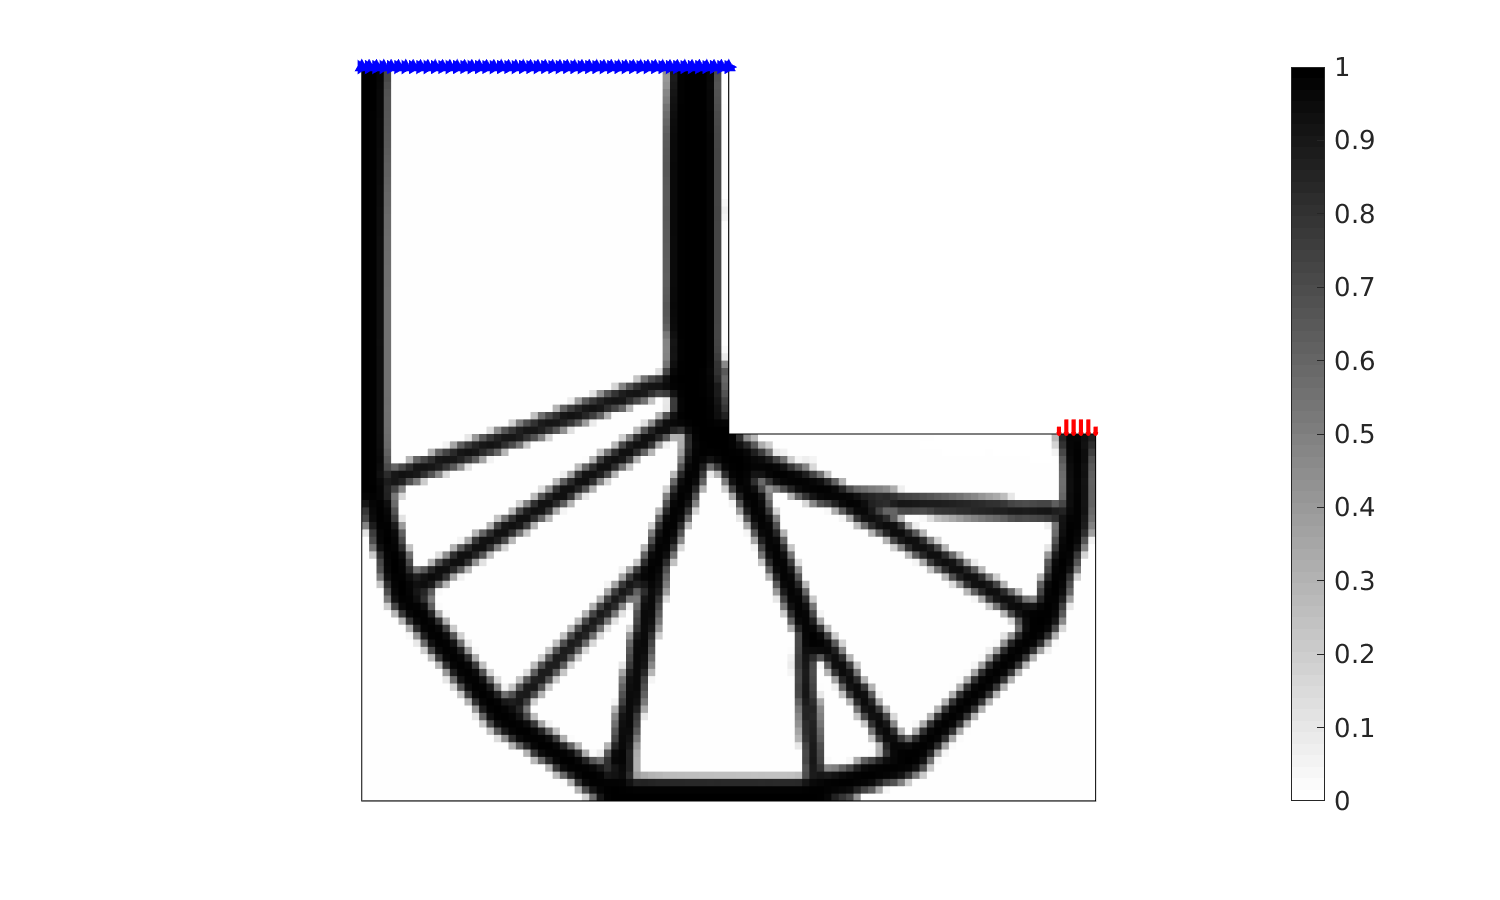
\includegraphics[width=0.45\textwidth]{images/Ch2/L-shapenelx_100nely_100_R_2_P_28_ft_3_Sl_0_9_KSldensity} }}%
\quad
\subfloat[von Mises plot $\sigma_{lim}=0.9$\label{fig.2.19b}]{{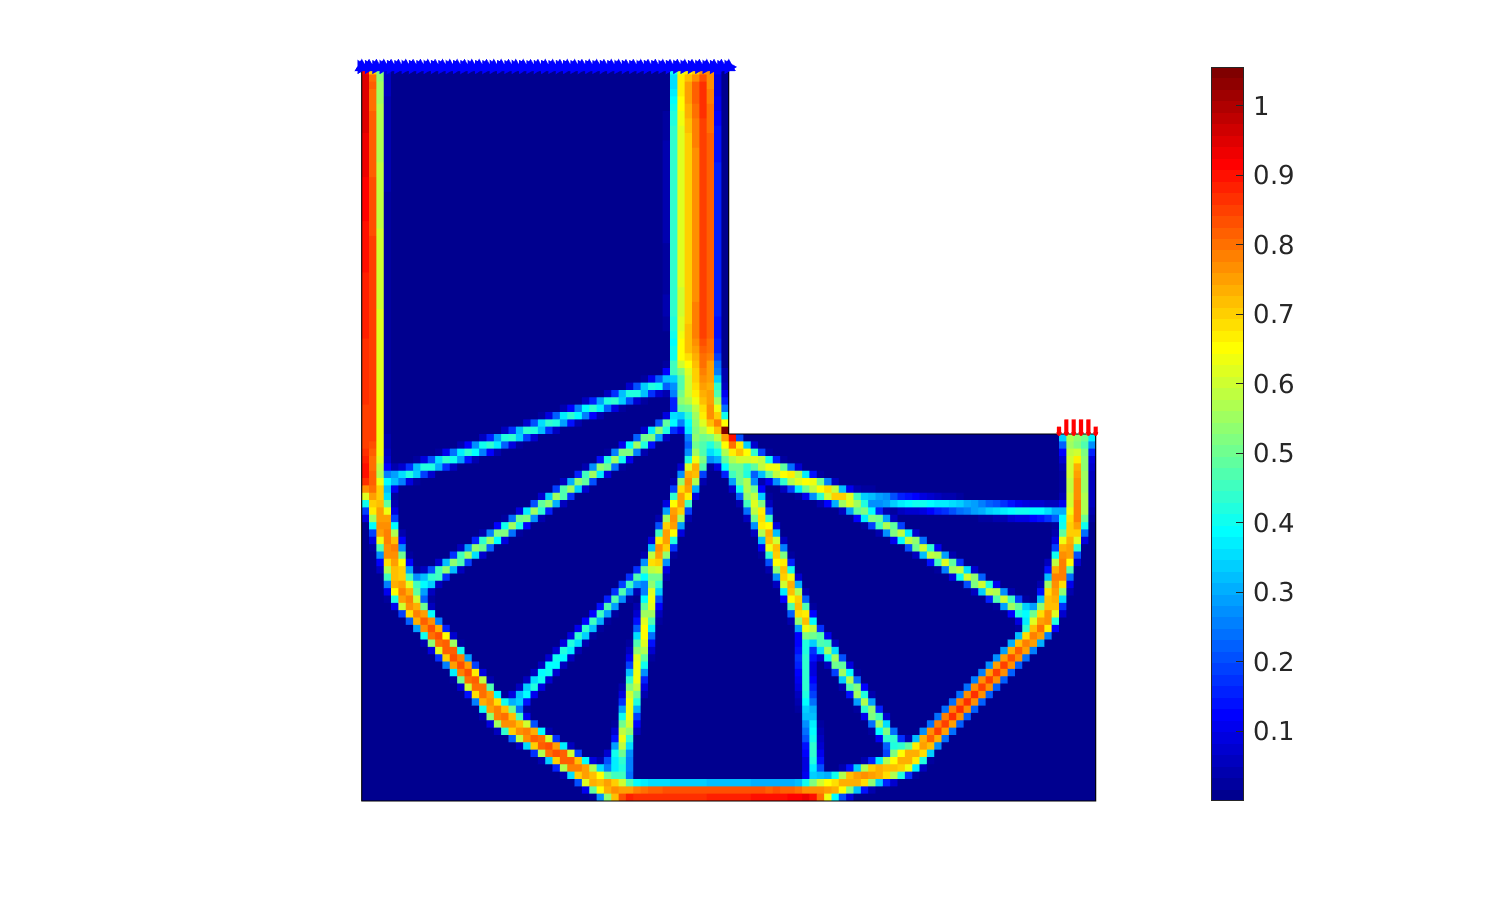
\includegraphics[width=0.45\textwidth]{images/Ch2/L-shapenelx_100nely_100_R_2_P_28_ft_3_Sl_0_9_KSlVM_stress} }}%
 \\
 \subfloat[Density plot $\sigma_{lim}=0.8$\label{fig.2.19d}]{{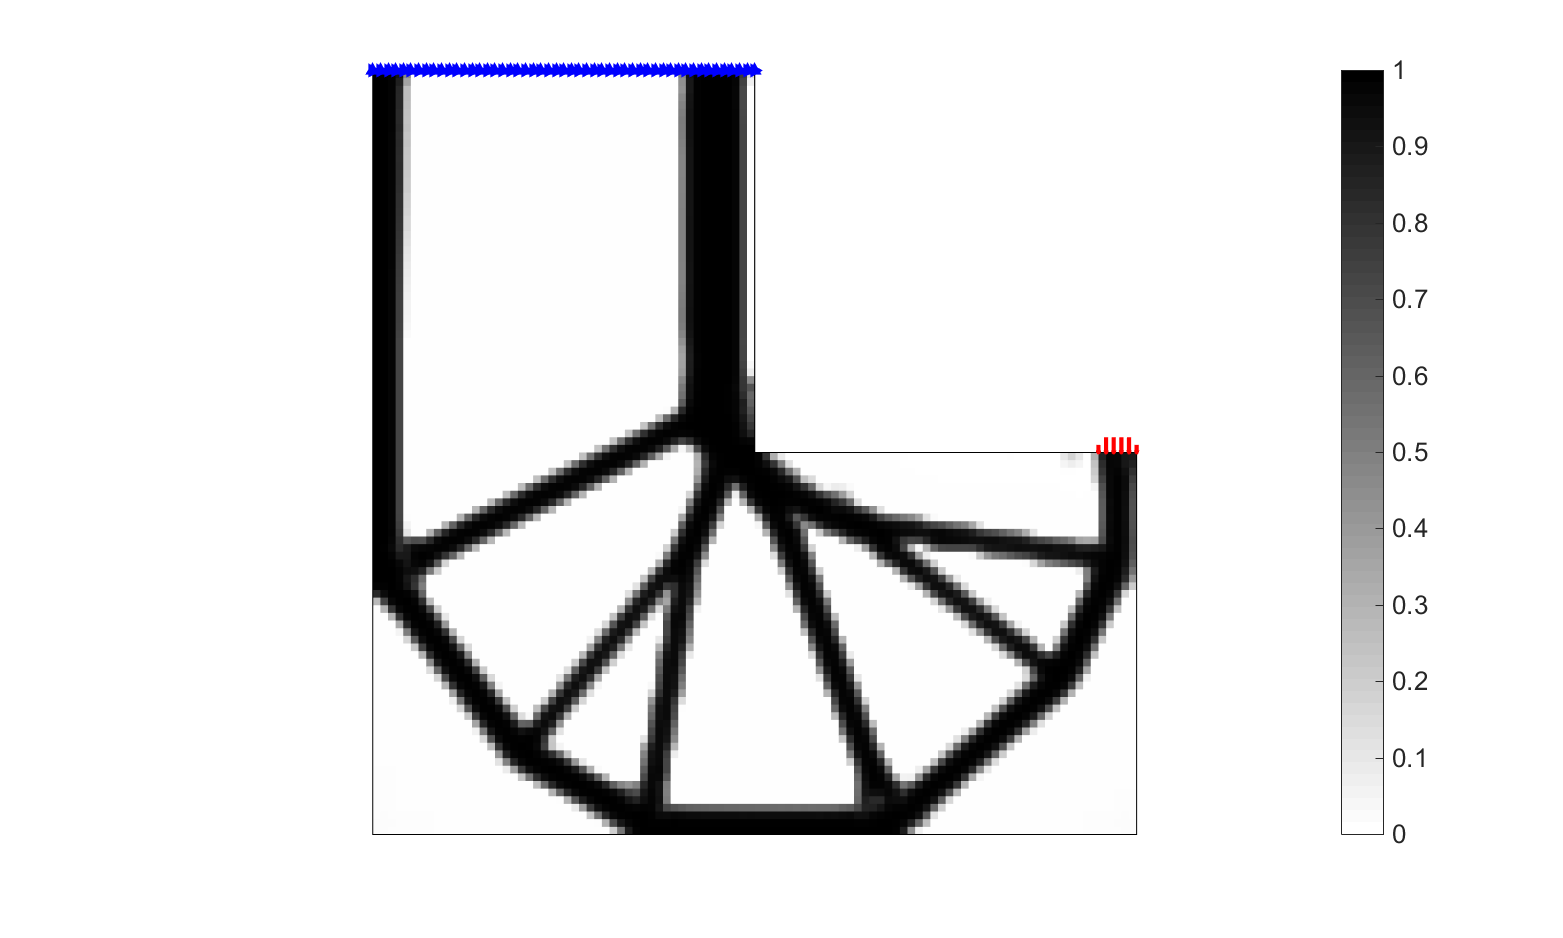
\includegraphics[width=0.45\textwidth]{images/Ch2/L-shapenelx_100nely_100_R_2_P_28_ft_3_Sl_0_8_KSldensity} }}%
 \quad
 \subfloat[von Mises plot $\sigma_{lim}=0.8$\label{fig.2.19e}]{{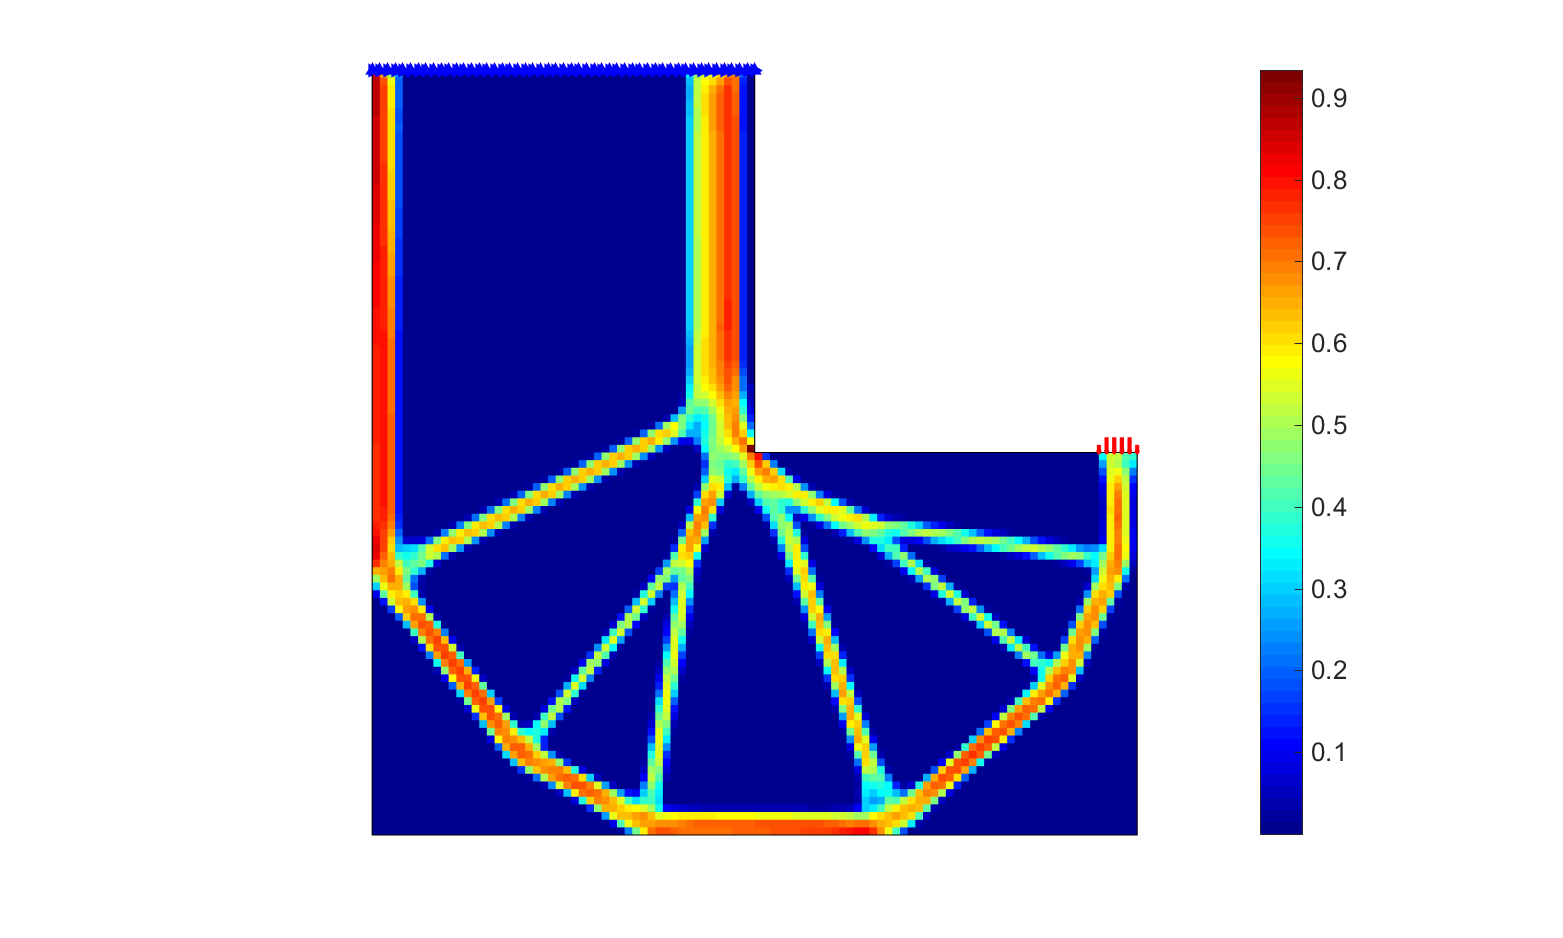
\includegraphics[width=0.45\textwidth]{images/Ch2/L-shapenelx_100nely_100_R_2_P_28_ft_3_Sl_0_8_KSlVM_stress} }}%
 \\
 \subfloat[Convergence plot $\sigma_{lim}=0.9$\label{fig.2.19c}]{{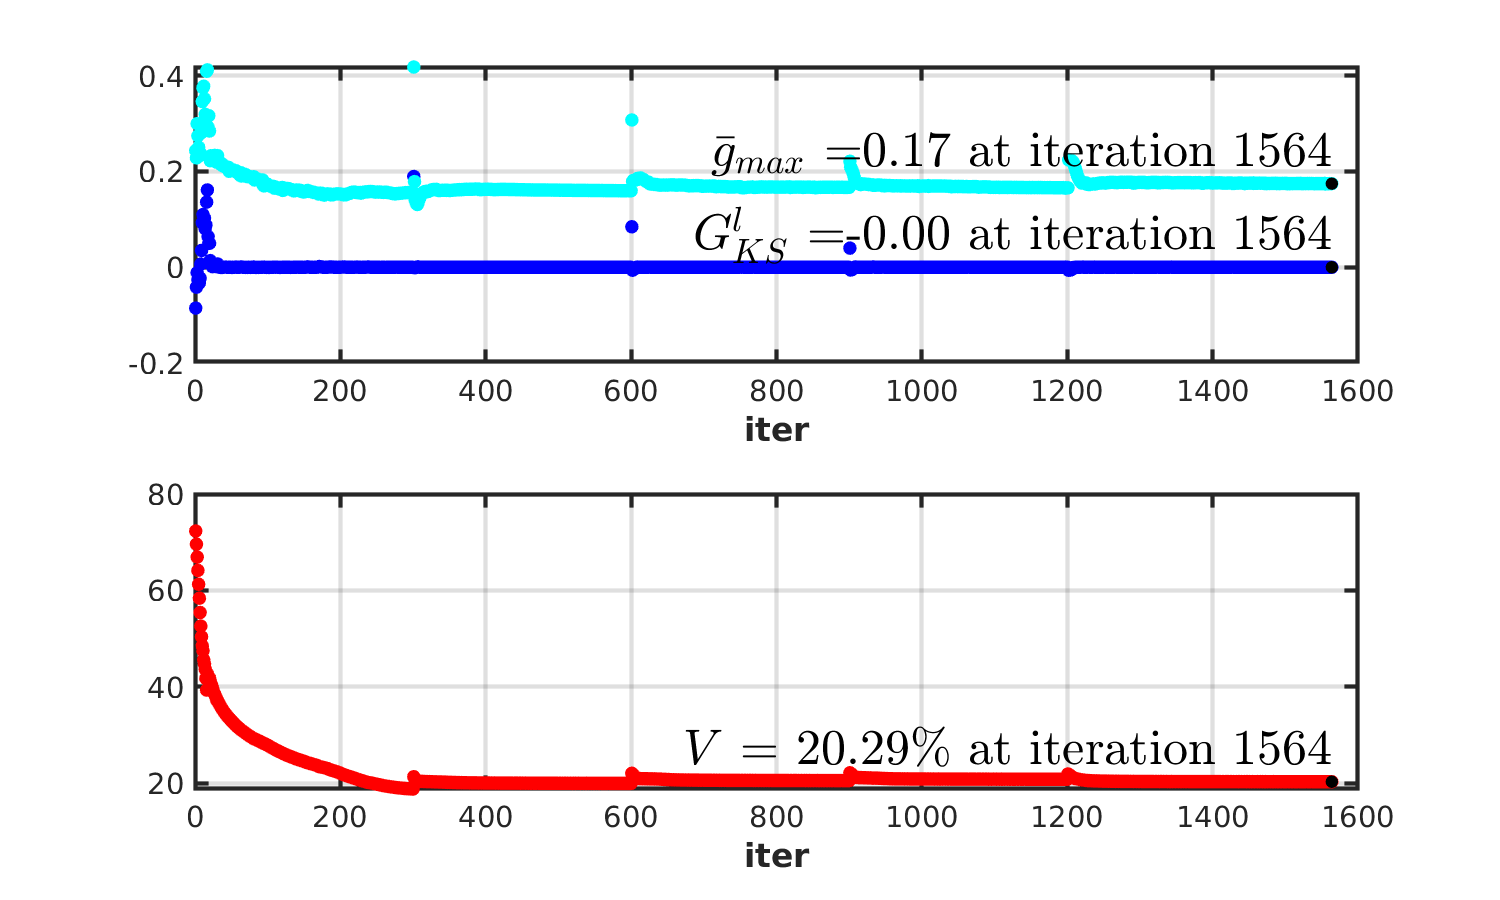
\includegraphics[width=0.45\textwidth]{images/Ch2/L-shapenelx_100nely_100_R_2_P_28_ft_3_Sl_0_9_KSlconvergence} }}%
     \quad
     \subfloat[Convergence plot $\sigma_{lim}=0.8$\label{fig.2.19f}]{{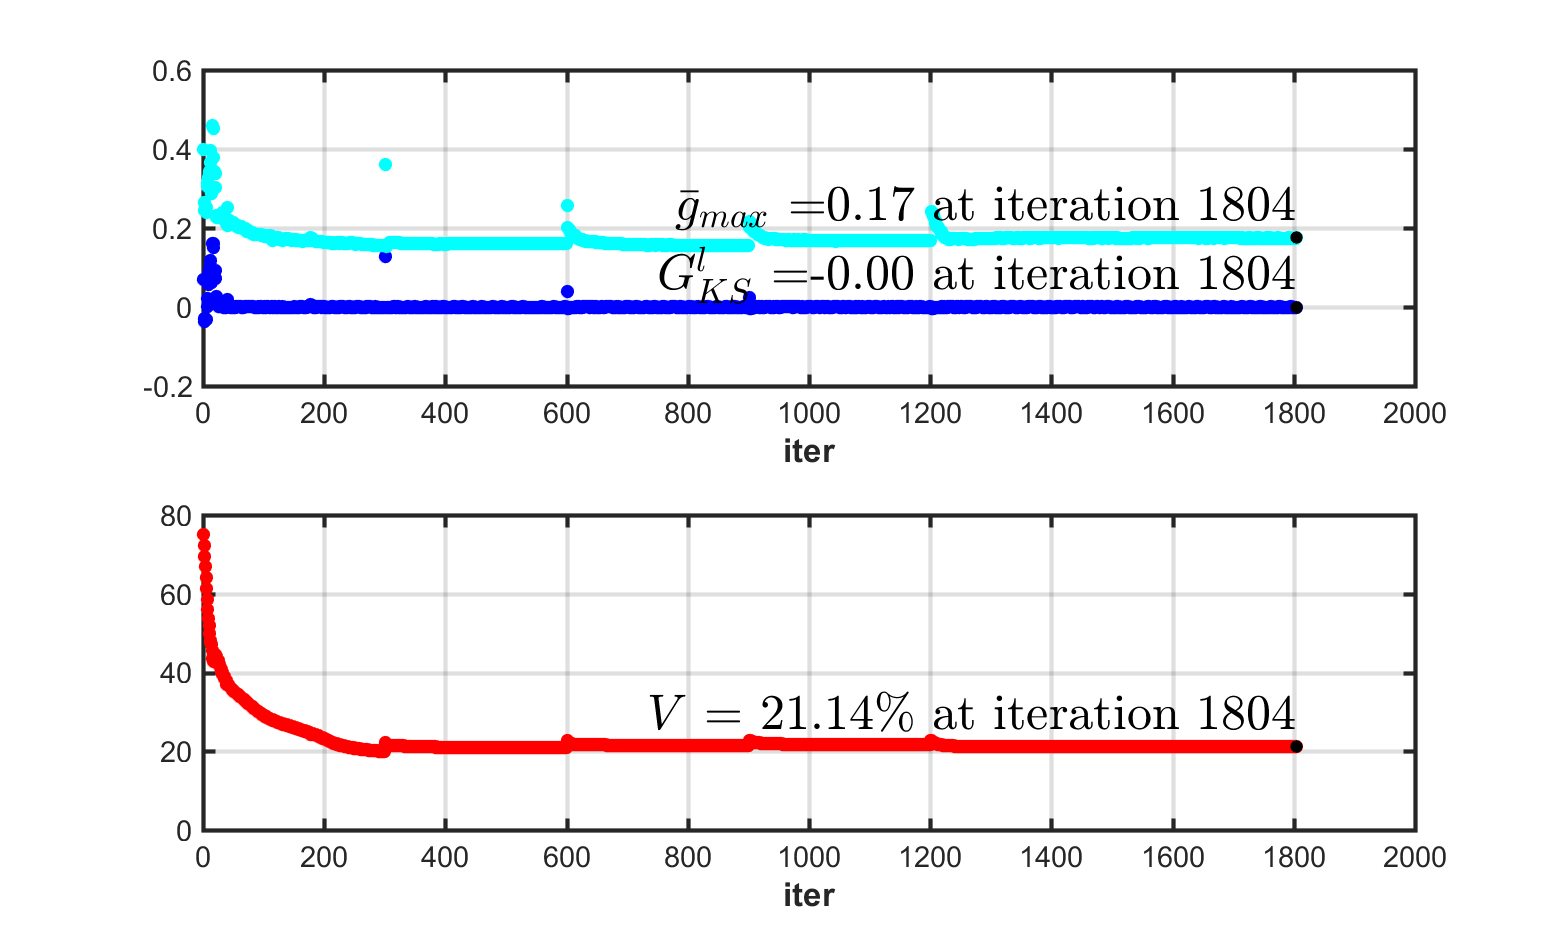
\includegraphics[width=0.45\textwidth]{images/Ch2/L-shapenelx_100nely_100_R_2_P_28_ft_3_Sl_0_8_KSlconvergence} }}%
  \\
\caption{L-shape $100\times 100$ mesh resolution, stress based topology optimization results. Density distribution, von Mises stress distribution and convergence history for $P=28$ and for $\sigma_{lim}=0.8,0.9$. }%
\label{fig.2.19}%
\end{figure*}
\begin{figure*}[h!]
\centering
\subfloat[Density plot $50 \times 50$\label{fig.2.20a}]{{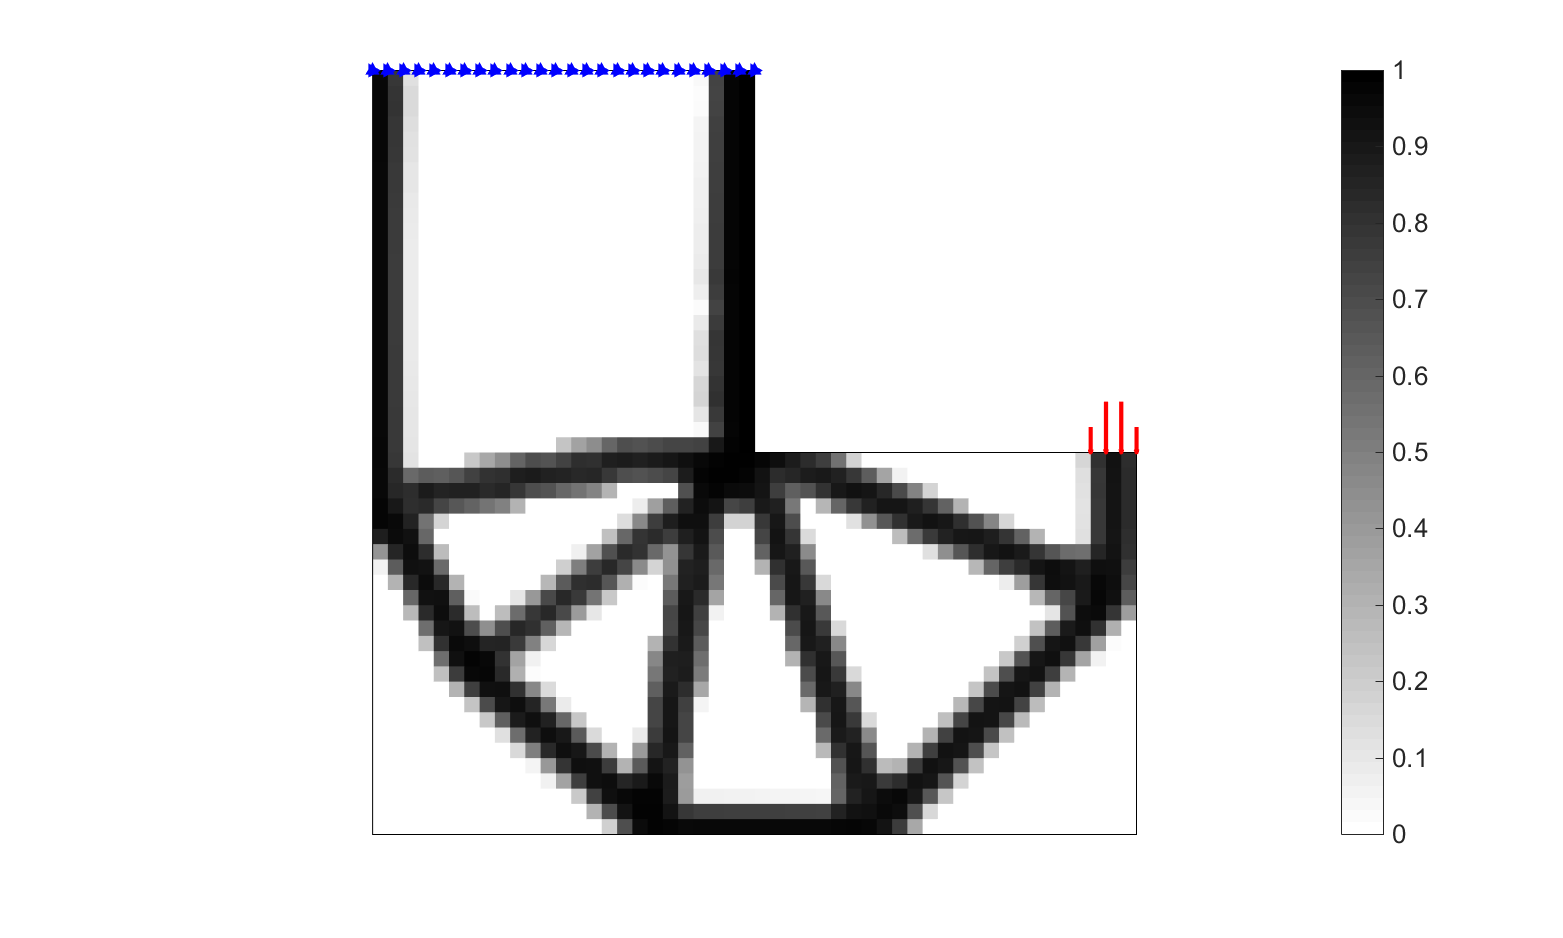
\includegraphics[width=0.45\textwidth]{images/Ch2/L-shapenelx_50nely_50_R_2_P_28_ft_3_Sl_1_KSldensity} }}%
\quad
\subfloat[von Mises plot $50 \times 50$\label{fig.2.20b}]{{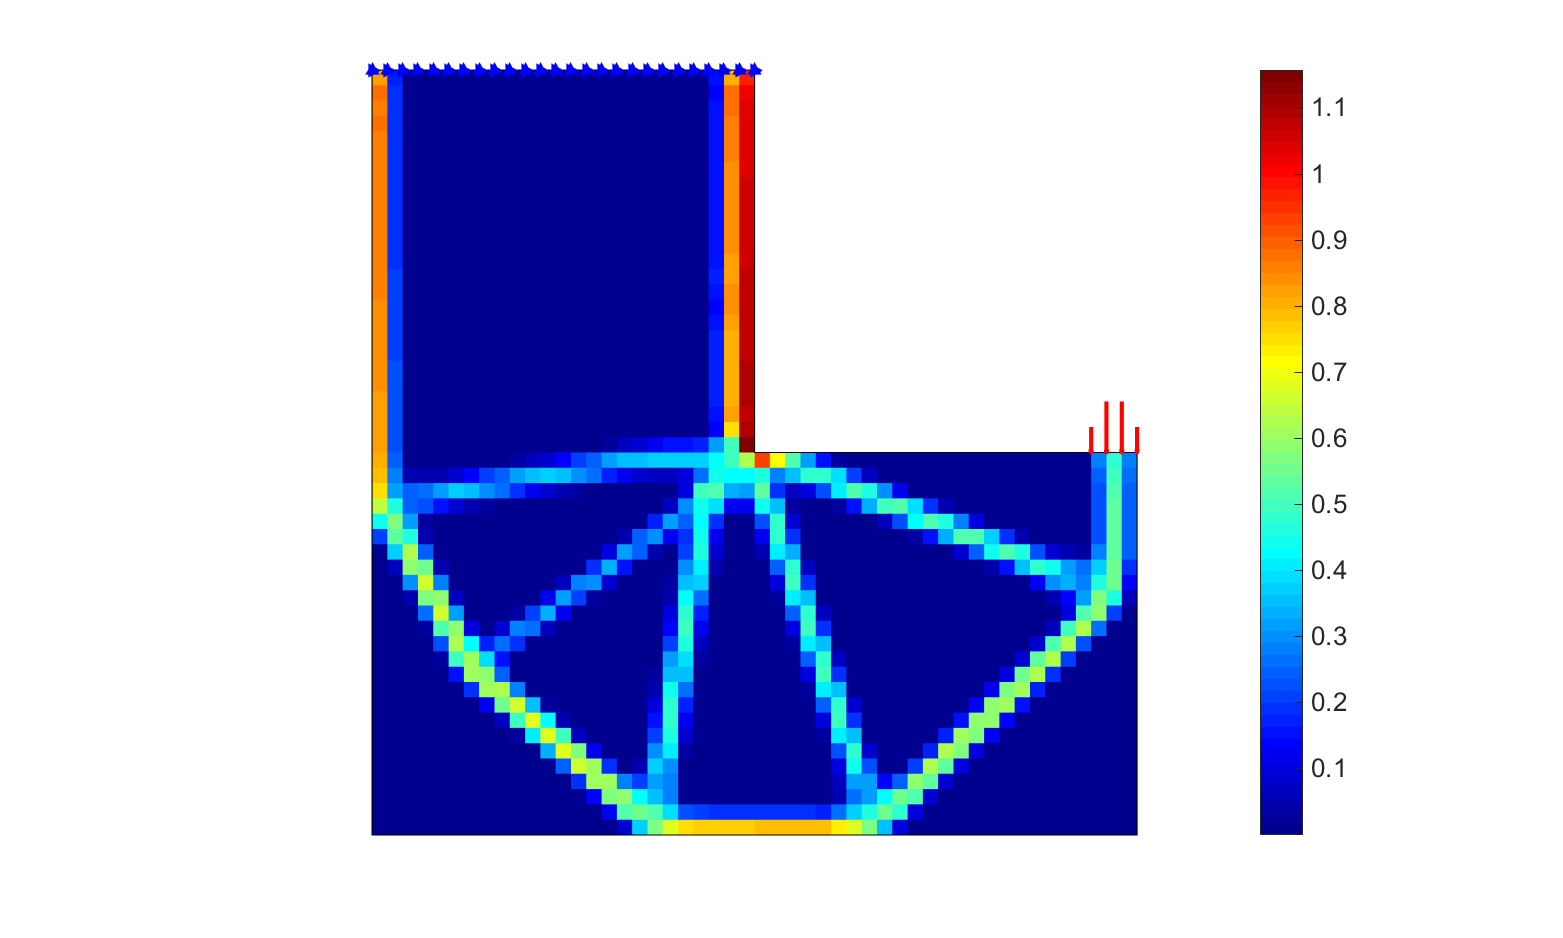
\includegraphics[width=0.45\textwidth]{images/Ch2/L-shapenelx_50nely_50_R_2_P_28_ft_3_Sl_1_KSlVM_stress} }}%
 \\
 \subfloat[Density plot $200 \times 200$\label{fig.2.20d}]{{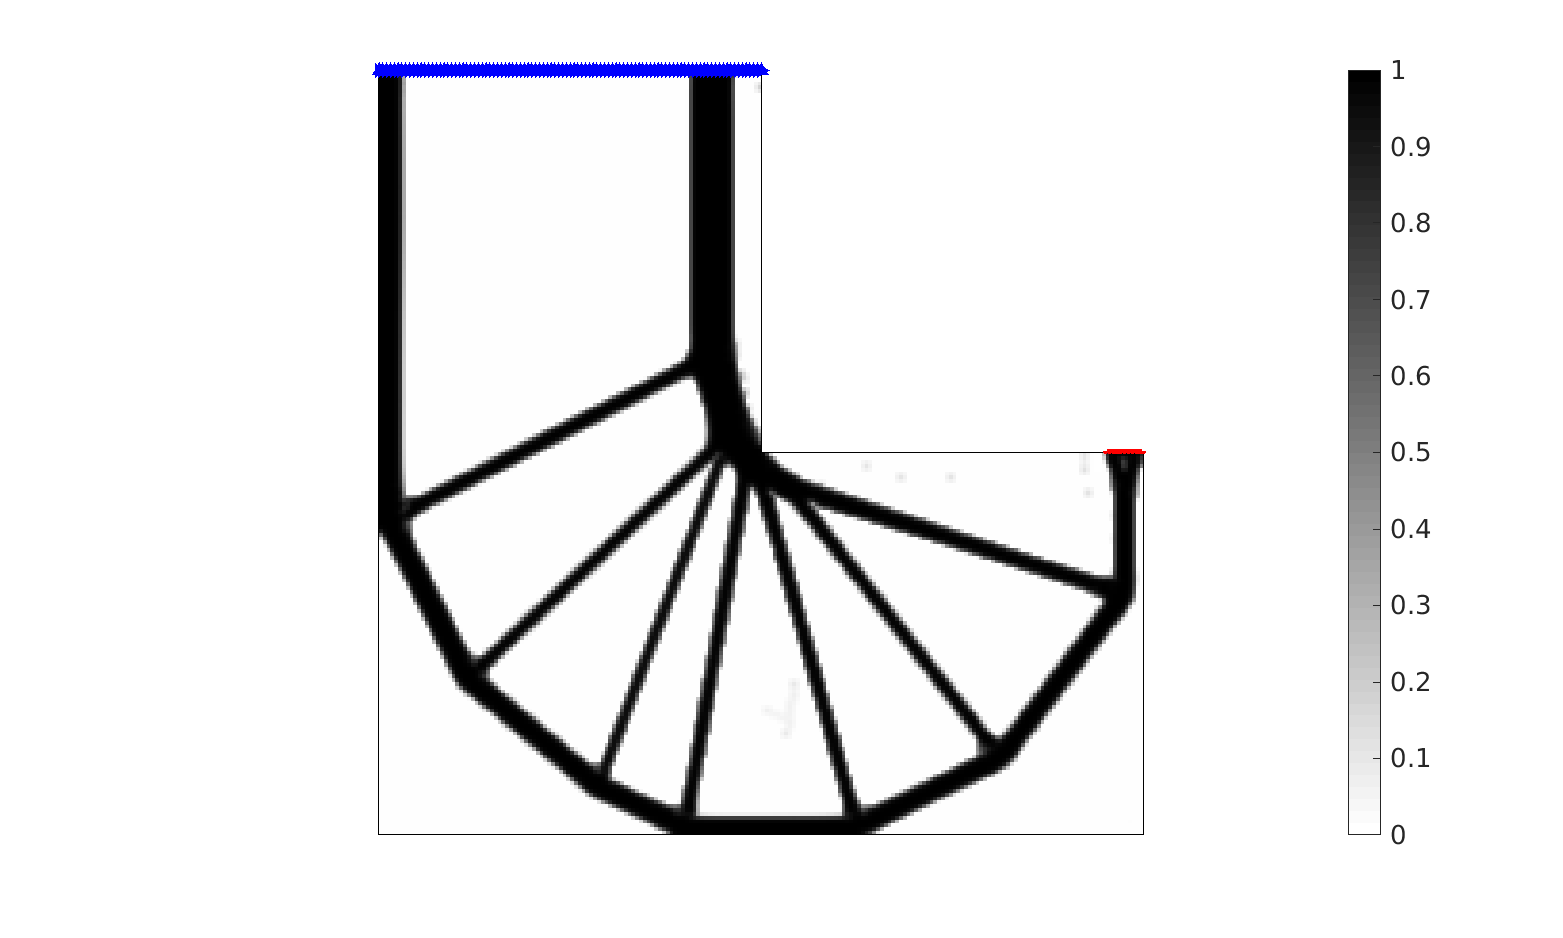
\includegraphics[width=0.45\textwidth]{images/Ch2/L-shapenelx_200nely_200_R_2_P_28_ft_3_Sl_1_KSldensity} }}%
 \quad
 \subfloat[von Mises plot $200 \times 200$\label{fig.2.20e}]{{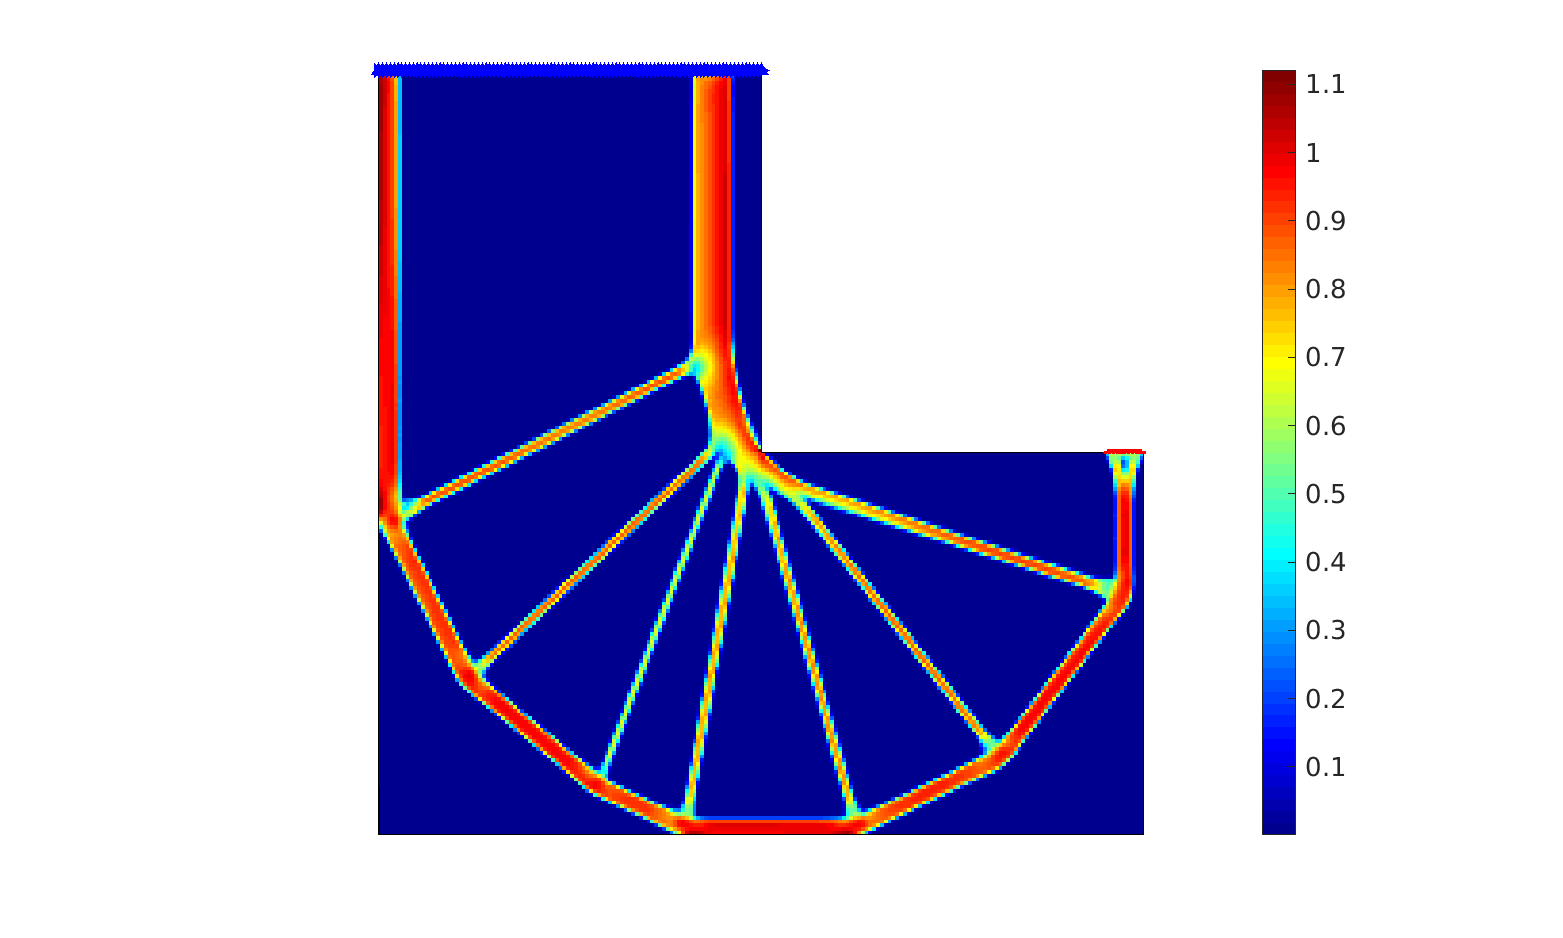
\includegraphics[width=0.45\textwidth]{images/Ch2/L-shapenelx_200nely_200_R_2_P_28_ft_3_Sl_1_KSlVM_stress} }}%
 \\
 \subfloat[Convergence plot $50 \times 50$\label{fig.2.20c}]{{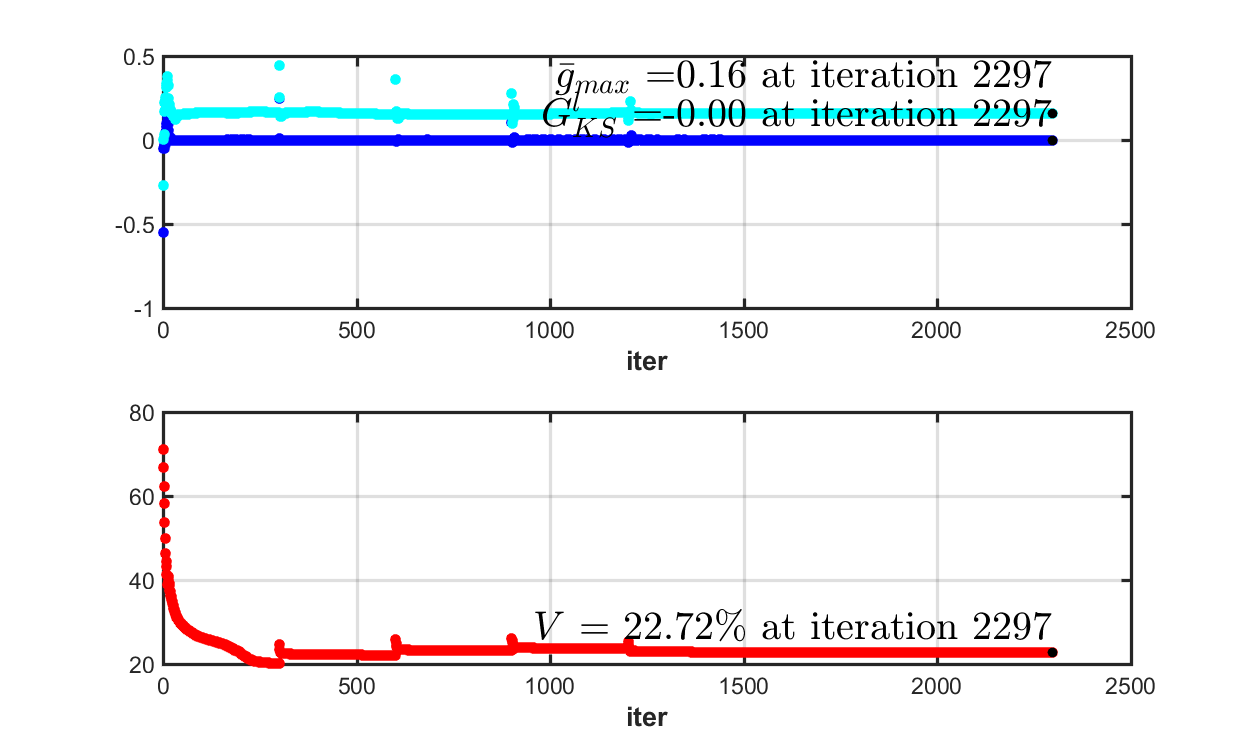
\includegraphics[width=0.45\textwidth]{images/Ch2/L-shapenelx_50nely_50_R_2_P_28_ft_3_Sl_1_KSlconvergence} }}%
     \quad
     \subfloat[Convergence plot $200 \times 200$\label{fig.2.20f}]{{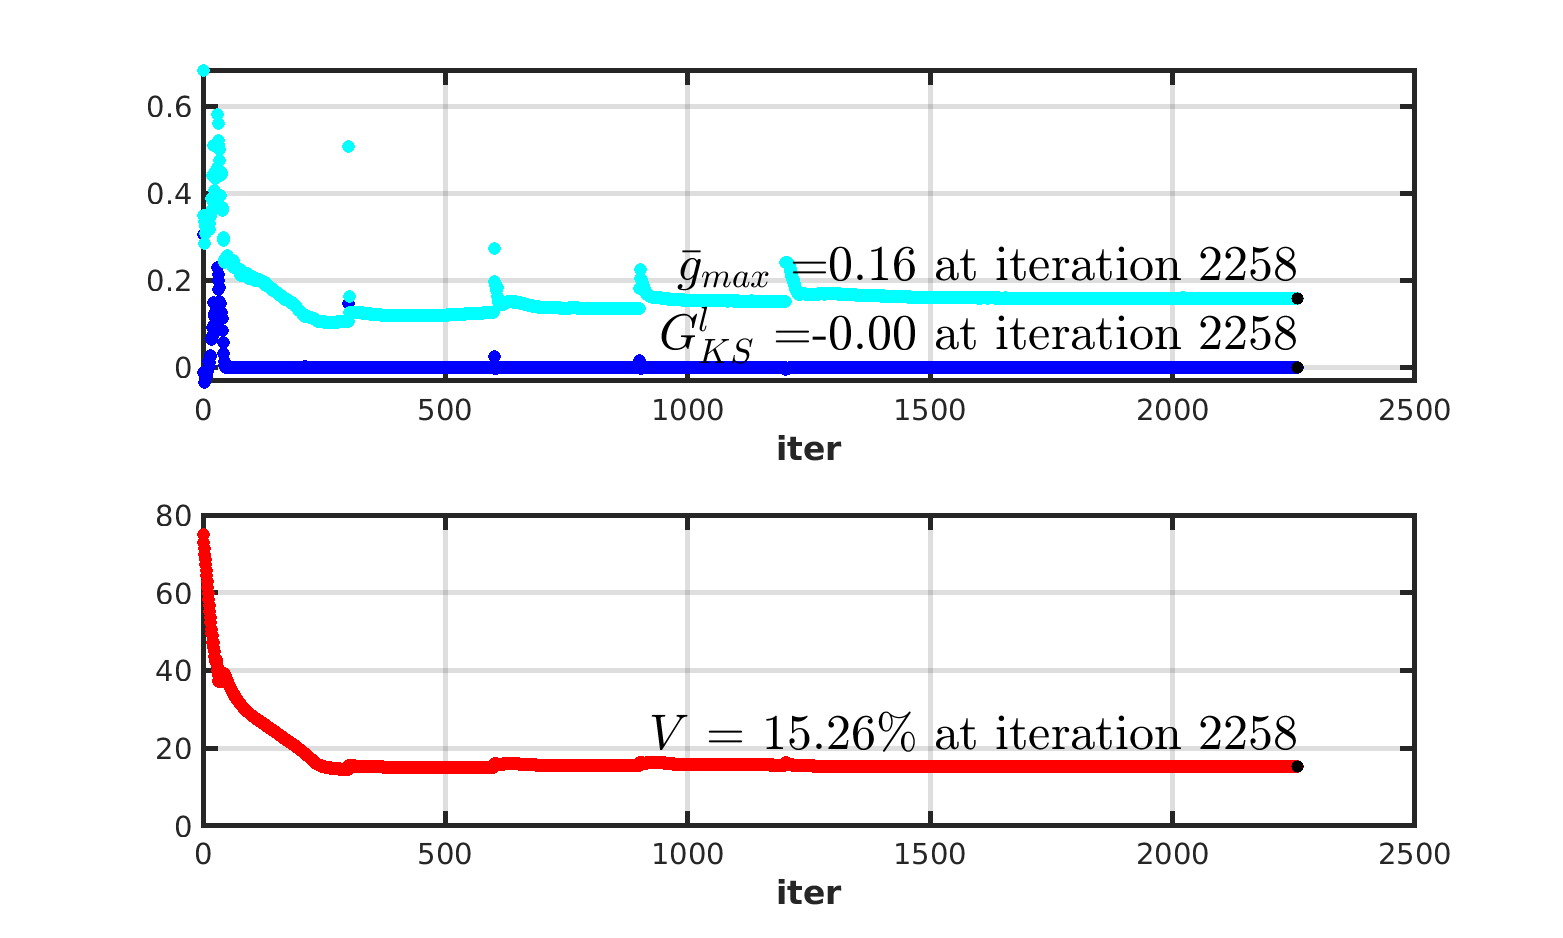
\includegraphics[width=0.45\textwidth]{images/Ch2/L-shapenelx_200nely_200_R_2_P_28_ft_3_Sl_1_KSlconvergence} }}%
  \\
\caption{L-shape $50\times 50$ and $200\times 200$ mesh resolutions, stress based topology optimization results. Density distribution, von Mises stress distribution and convergence history for $P=28$ and for $\sigma_{lim}=1$. }%
\label{fig.2.20}%
\end{figure*}
\clearpage
Finally in figure \ref{fig.2.20} the effect of mesh resolution is represented. The solutions are different for different meshes. This may be caused again by the optimization problem non convexity and more probably by the FEM convergence for the stress analysis. The final maximum stress seems to be not affected by the number of elements in the discretization. This may seems to not be in accordance with equation \ref{ee20}. In reality this is due to the FEM improved accuracy, to the fact that different local minima are attained and to the fact that for finer meshes the stress peak could be attained in several Gauss point, attenuating the increase of distance from the actual $\bar{g}_{max}$ that was expected due to equation \ref{ee20}.
\subsection{Dealing with multiple load cases}
In many practical situations, a component will have to respect mechanical requirements in several operating conditions. When this is the case the topology optimization formulation needs to be modified to include such requirements simultaneously. In fact the best design for a given operating condition, can generally speaking be different from the best design with respect to another condition. Respecting the stress constraint for a loading condition will not prevent the structure from failing for another one. In the stress formulation \ref{formulation_stress}, the von Mises stress should be controlled for all Gauss point but also for all operating conditions. Unified approach \ref{Verbart_formulation} is adopted for each condition giving the following nonlinear programming problem:
\begin{equation}
\begin{cases}
\min_{\VectorVar{0}\leq\VectorVar{x}\leq\VectorVar{1}} {\VectorVar{|\Omega_{el}|}^T\VectorVar{x}} \\
\textit{s.t.}\\
(G^{l}_{KS})_{l_c}\leq 0 & \forall l_c=1,2,...,N_l \\
\end{cases}
\end{equation}
where $N_l$ is the number of operating conditions considered for the designed product. We make the hypothesis that in all operating condition the structural boundary conditions will not change and the only load applied to the structure will change. 
\begin{figure}[ht]
\centering
\subfloat[\label{fig.2.21a}]{{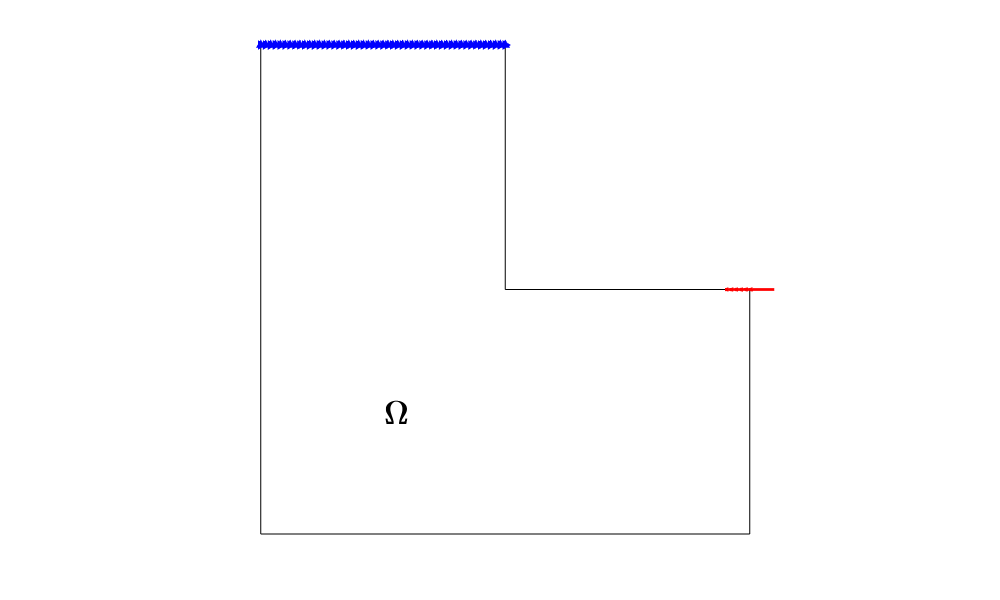
\includegraphics[width=0.45\textwidth]{images/Ch2/Design_problem_LC1} }}%
\quad
\subfloat[\label{fig.2.21b}]{{\includegraphics[width=0.45\textwidth]{images/Ch2/Design_problem_LC2} }}%
  \\
\caption{Multiple load cases applied to the L-shape, a) horizontal distributed load, b) vertical distributed load}%
\label{fig.2.21}%
\end{figure}
Under this hypothesis the FEA model will only have several right hand side vectors, each one corresponding to a physical loading situation. To enhance the numerical efficiency it is possible to consider again a smooth approximation of maximum function (a similar approach was proposed in \cite{le2010stress}) applied to all load cases that reduce the number of constraints to be considered in the optimization formulation:
\begin{equation}
\begin{cases}
\min_{\VectorVar{0}\leq\VectorVar{x}\leq\VectorVar{1}} {\VectorVar{|\Omega_{el}|}^T\VectorVar{x}} \\
\textit{s.t.}\\
\frac{1}{P_l}\log{\left(\frac{\sum_{l_c=1}^{N_l}e^{P_l(G^{l}_{KS})_{l_c}}}{N_l}\right)}\leq 0 \\
\end{cases}
\end{equation}
\begin{figure*}[ht]
\centering
\subfloat[\label{fig.2.22a}]{{\includegraphics[width=0.45\textwidth]{images/Ch2/MLCSnelx_100nely_100_R_2_P_10_ft_3_Sl_1_KSldensity} }}%
\quad
\subfloat[\label{fig.2.22b}]{{\includegraphics[width=0.45\textwidth]{images/Ch2/MLCSnelx_100nely_100_R_2_P_10_ft_3_Sl_1_KSlconvergence} }}%
  \\
  \subfloat[\label{fig.2.22c}]{{\includegraphics[width=0.45\textwidth]{images/Ch2/MLCSnelx_100nely_100_R_2_P_10_ft_3_Sl_1_KSlVM_stress_1} }}%
  \quad
  \subfloat[\label{fig.2.22d}]{{\includegraphics[width=0.45\textwidth]{images/Ch2/MLCSnelx_100nely_100_R_2_P_10_ft_3_Sl_1_KSlVM_stress_2} }}%
    \\
\caption{Results for the multiple load case study of an L-shape for a $100\times100$ mesh. a) density plot, b) convergence plot, c)-d) von Mises stress plot for the first and the second load case respectively. }%
\label{fig.2.22}%
\end{figure*}
One can observe that with this formulation one includes a double error approximating the maximum, therefore the choice of $P_l$ and $P$ should be a good compromise between response non-linearity and maximum stress approximation accuracy.
To show an application of this approach we considered an L-shape design problem under 2 load cases c.f. figure \ref{fig.2.21}.
For this study we chose $P=10$ and $P_l=4$. And the same settings of table \ref{tab:2.2}. The study was conducted for a $100\times100$ mesh and the results are reported in figure \ref{fig.2.22}. The continuation strategy successfully enforces a black and white design in the solution c.f. figure \ref{fig.2.22a}. On the other hand the convergence history was quite longer than the one experienced for the single load case stress based topology optimization and this is probably due to the additional non-linearity induced by load case aggregation. The nested use of KS aggregation reduces the number of design constraint responses but cumulate the effect of nonlinearity of both stress and load case aggregation. In figures \ref{fig.2.22c}  and \ref{fig.2.22d} one can observe von Mises stress distribution of the solution under each load case. It can be observed that the first load case adds some load paths that activate only in the first load case alleviating the maximal stress.
The second load case is the most constraining with the final constraint violation of 0.51 in the second load case and of 0.3 in the first one. This is due to the consecutive KS aggregations that sum their approximation error. A continuation strategy to deal with such scenarios is proposed in section \ref{IS}.


\section{SIMP application to the pylon and engine mount design}
\label{SIMP_application}
A civil aircraft Powerplant System (PPS) primary structure has as a primary function to attach the engine to the aircraft wing. Furthermore the design of all the components of the PPS, ( pylon, engine mounts and nacelle) has also significant importance on the final integrated engine performance.
For example the variation of the radial clearances at the blade tip of each stage (tip-clearances) affects engine time on wing, compressor surge margin and the thrust specific fuel consumption \cite{lattime2002turbine,benito20083d}. Controlling the tip clearance variation due to engine maneuvers is for these reasons a major criterion considered during the PPS design. Including engine performance in the pylon design loop was investigated in Bettebghor et al. \cite{bettebghor2013bi}. In that study both engine casing and pylon sizing optimization were simultaneously tackled in order to find a better mass distribution between engine and PPS structures, while achieving a feasible design. On the other hand the engine mounts were considered in a fixed position so that only the engine casing thicknesses influenced directly tip clearances.
In this work we consider the optimization of the PPS structure under a fixed engine architecture.
 The engine pylon topology optimization was also treated in \cite{remouchamps2011application} considering both structural compliance under several load cases and aerodynamic drag.
 In Xue et al. \cite{xue2012structural} an Ant Colony Algorithm is deployed to optimize the front pylon mounts on the base of average stress under multiple load cases.
 In this work we don't focus on pylon aerodynamic performance, as it was done in \cite{remouchamps2011application}, since we fixed the design space shape. On the other hand we include the pylon to engine interface inside the design zone. This gives the solution more freedom that is also necessary to have an impact on both engine deformations and PPS primary structure mass. The design zone is much larger than the one considered in \cite{xue2012structural} and we didn't employ Ant Colony Algorithm to tackle the optimization problem.
 The optimization formulation adopted for this work is a mass minimization with both stress and engine performance constraints. The fact of including these constraints is beneficial for the total lead time in the design process. In this way, the solution provided by the topology optimization phase will need minor modifications in order to achieve a feasible design that should satisfy both stress and performance requirements. This comes however at increased computational cost as the gradients of these two new constraints have to be computed.\\
 The engine and the design zone (c.f. figure \ref{f.1}) are connected using an elimination approach that we developed in subsection \ref{sssec332}. The final stiffness matrix of the entire model can then be directly assembled as:
 \begin{equation}
 \label{eq.9}
 \left[K(\lbrace x\rbrace)\right]=\left[K_{DZ}(\lbrace x\rbrace)\right] + \left[K_{E}\right]
 \end{equation}
 From here on, we will refer to $\left[K(\lbrace x\rbrace)\right]$ as the stiffness matrix after the application of boundary conditions and to $\left[K_{E}\right]$ as the contribution of the engine stiffness to  $\left[K(\lbrace x\rbrace)\right]$.
 In the same way one can make the assembly of the load vector matrix as:
 \begin{equation}
 \label{eq.10}
  \MatrixVar{F(\lbrace x\rbrace)} = \MatrixVar{ F_{DZ}(\lbrace x\rbrace)}+ \MatrixVar{ F_{E} }
 \end{equation}
 Where $\MatrixVar{ F_{DZ}(\lbrace x\rbrace) } $ is the matrix whose columns are load vectors coming from the design zone that can depend on the configuration\footnote{This is the case of acceleration induced load that depends on the mass of the solution and so on the configuration given by the design vector $\lbrace x\rbrace$.} and $\MatrixVar{ F_{E} } $ is the matrix whose columns are load vectors applied on the engine model.
 The static balance equations will be written as:
 \begin{equation}
 \label{sbeq}
 \left[K(\lbrace x\rbrace)\right]\MatrixVar{ U (\lbrace x\rbrace) } = \MatrixVar{ F(\lbrace x\rbrace)}
 \end{equation}
 The so computed displacement matrix $\MatrixVar{ U (\lbrace x\rbrace)}$ is employed for the evaluation of design zone von Mises stress and  the TSFC variation (c.f. subsection \ref{ssec1.2.2}).
 The mass of the PPS structure is also an important parameter that we consider through the volume fraction defined as:
 \begin{equation}
 \label{eq.12}
 V\left(\lbrace x\rbrace\right)=\frac{\sum_{i=1}^{N_{el}}x_i|\Omega_i|}{\sum_{i=1}^{N_{el}}|\Omega_i|}=\frac{\lbrace|\Omega|\rbrace^T\lbrace x\rbrace }{\lbrace|\Omega|\rbrace^T\lbrace \mathbf{1}\rbrace}
 \end{equation}
 Where $|\Omega_i|$ is the Volume of the $i^{th}$ element,$\lbrace|\Omega|\rbrace$ is the vector containing the volume of each element and $\lbrace \mathbf{1}\rbrace$ is the vector having the same length of $\lbrace x\rbrace$ with 1 for each row.
 The value of $V\left(\lbrace x\rbrace\right)$ is between 0 and 1 and gives the fraction of volume that is filled by active material.
 The final design should be as light as possible and should reduce the engine consumption variation induced by aircraft maneuvers.   
 To get reasonable results the von Mises stress in the design zone should also be lower than an allowable value.
 The full problem can thus be written as a non-linear constrained optimization problem (c.f. Eq. \ref{topoeq} for one load case), seeking to minimize the mass of the PPS structure, while imposing constraints on TSFC variations and maximum von Mises stress.
 \begin{equation}
 \label{topoeq}
 \left\lbrace\begin{array}{cc}
 \underset{\lbrace x\rbrace}{\min} V\left(\lbrace x\rbrace\right)& \\
 s.t. & \\ 0\leq x_i \leq 1  & \forall i=1,2,\dots,N_{el}\\
 G_T\left(\lbrace U\left(\lbrace x\rbrace\right)\rbrace\right)=\frac{\Delta TSFC \%\left(\lbrace U\left(\lbrace x\rbrace\right)\rbrace\right)-T_0}{T_0}\times 100 \leq 0 & \\
 \left[K\left(\lbrace x\rbrace\right)\right]\lbrace U \left(\lbrace x\rbrace\right) \rbrace = \lbrace F \left(\lbrace x\rbrace\right)\rbrace & \\
 (\sigma_{VM})_j\left(\lbrace x\rbrace,\lbrace U\left(\lbrace x\rbrace\right)\rbrace\right) \leq \sigma_{lim}  & \forall j| x_{i(j)}> 0
 \end{array}\right.
 \end{equation}
 Where the $(\sigma_{VM})_j$ is the von Mises stress computed in the j-th Gauss point and $x_{i(j)}$ is the pseudo density of the i-th element that contains the j-th quadrature point, and $\sigma_{lim}$ represents the allowable von Mises stress in the design zone and $T_0$ is an allowable overconsumption due to the maneuver load case. Classical compliance minimization formulation is cheaper than our proposed formulation, and can be adopted to get the inspiration for novel designs. Nevertheless the stiffest design will not always be able to respect both stress and engine consumption specifications. For this reason the formulation of equation \ref{topoeq}, that also includes engine performance and stress constraints will be considered for the rest of this study.
 To evaluate the microscopic stress tensor in each Gauss point of the design zone, in the stiffness assembly phase the product of stress deformation matrix $\left[D\right]|_{x=1}$ and of the displacement-deformation matrix $\left[B\right]$ has to be saved in  $\left[DB\right]$. This large sparse matrix reads in terms of input a displacement vector and provides as an output a stress vector containing 6 stress tensor components  for each Gauss point of the design zone:
 \begin{equation}
 \label{e.24}
 \lbrace\bar{\sigma}\left(\lbrace U\left(\lbrace x\rbrace\right)\rbrace\right)\rbrace=\left[DB\right]\lbrace U(\lbrace x \rbrace\rbrace
 \end{equation}
  The von Mises stress in 3D is then:
  \begin{equation}
  \label{e.20}
  \sigma_{VM}=\sqrt{\sigma_{xx}(\sigma_{xx}-\sigma_{yy})+\sigma_{yy}(\sigma_{yy}-\sigma_{zz})+\sigma_{zz}(\sigma_{zz}-\sigma_{xx})+3(\tau_{xy}^2+\tau_{yz}^2+\tau_{zx}^2)}
  \end{equation}
Using the same step adopted for the 2D use case (c.f. equations \eqref{eq.2.30}, \eqref{eq.2.32})
, the satisfaction of stress constraints is thus imposed in problem (\ref{topoeq}) as:
\begin{equation}
\label{topoeq2}
\left\lbrace\begin{array}{cc}
\underset{\lbrace x\rbrace}{\min} V\left(\lbrace x\rbrace\right)& \\
s.t. & \\ 0\leq x_i \leq 1  & \forall i=1,2,\dots,N_{el}\\
G_T\left(\lbrace U\left(\lbrace x\rbrace\right)\rbrace\right)=\frac{\Delta TSFC \%\left(\lbrace U\left(\lbrace x\rbrace\right)\rbrace\right)-T_0}{T_0}\times 100 \leq 0 & \\
\left[K\left(\lbrace x\rbrace\right)\right]\lbrace U \left(\lbrace x\rbrace\right) \rbrace = \lbrace F \left(\lbrace x\rbrace\right)\rbrace & \\
G^{l}_{KS}(\lbrace x\rbrace,\lbrace U\left(\lbrace x\rbrace\right)\rbrace)\leq 0
\end{array}\right.
\end{equation}
 \subsection{Sensitivity computation}
 \label{subsec2.4}
 In this subsection we detail the computation of responses sensitivities in problem (\ref{topoeq2}). The reader can observe that a major complexity with respect to the 2D use-case comes from the fact that the mesh is non uniform.
  It is straightforward to use equations \eqref{eq.2.46} and \eqref{eq.2.47} to compute $\left\lbrace\frac{d G_T}{dx}\right\rbrace$, $\left\lbrace\frac{d V}{dx}\right\rbrace$ and $\left\lbrace\frac{d G_{KS}^l}{dx}\right\rbrace$. Let's start by the evaluation of the TSFC variation constraint $G_T$. Since $ \Delta TSFC \%$ has no direct dependency on the $\lbrace x_{Phys}\rbrace$ we have:
    \begin{equation}
   \left \lbrace\frac{\partial G_T}{\partial x_{Phys}}\right \rbrace=\lbrace 0\rbrace 
    \end{equation}
     By the use of equations \ref{e.3},\ref{e.4} and \ref{e.5}:
    \begin{equation}
      \left \lbrace\frac{\partial G_T}{\partial U}\right \rbrace=\frac{100 }{T_0}\left \lbrace\frac{\partial \Delta TSFC \%}{\partial U}\right \rbrace =\frac{100 }{T_0}\sum_{s=1}^{ns}\lambda_{(s)}\left \lbrace\frac{\partial R_{(s)}}{\partial U}\right \rbrace=\frac{100}{T_0}\sum_{s=1}^{ns}\frac{\lambda_{(s)}}{N_{(s)}R_{(s)}}\left[\gamma_{(s)}\right] ^T\delta_{(s)}
       \end{equation}
       Similarly, since $V$ is only dependent on $x_{Phys}$:
 \begin{equation}
           \left\lbrace\frac{\partial V}{\partial U}\right\rbrace=\lbrace 0\rbrace 
 \end{equation}
 By the use of equation \eqref{eq.12}:
    \begin{equation}
                     \left\lbrace\frac{\partial V}{\partial x_{Phys}}\right\rbrace=\frac{\lbrace|\Omega|\rbrace}{\lbrace|\Omega|\rbrace^T\lbrace \mathbf{1}\rbrace}
     \end{equation}
 For the lower bound Kreisselmeier-Steinhauser
 function sensitivities we have both dependency on $\lbrace x_{Phys}\rbrace$ and $\lbrace U (\lbrace x_{Phys}\rbrace) \rbrace$: 
   \begin{equation}
   \left\lbrace\frac{\partial G^{l}_{KS}}{\partial x_{Phys}}\right\rbrace=\frac{\sum_{i=1}^{N_G}\left\lbrace\frac{\partial \bar{g}_i}{\partial x_{Phys}}\right \rbrace e^{P\bar{g}_i}}{\sum_{i=1}^{N_G}e^{P\bar{g}_i}}
   \end{equation}
   With $ \left\lbrace\frac{\partial \bar{g}_i}{\partial x_{Phys}}\right \rbrace$ defined as:
   \begin{equation}
   \left\lbrace\frac{\partial \bar{g}_i}{\partial x_{Phys}}\right \rbrace_j=\left\lbrace\begin{array}{cc}
   \frac{(\sigma_{VM})_i}{\sigma_{lim}}-1& i \in \mathbf{G}_j\\
   0 &  i \notin  \mathbf{G}_j
   \end{array}\right.
   \end{equation}
   $\mathbf{G}_j$ referred to the j-th element Gauss point index. In the same way one can evaluate:
   \begin{equation}
   \label{e.32}
   \left\lbrace\frac{\partial G^{l}_{KS}}{\partial U}\right\rbrace=\frac{\sum_{i=1}^{N_G}\left\lbrace\frac{\partial \bar{g}_i}{\partial U}\right \rbrace e^{P\bar{g}_i}}{\sum_{i=1}^{N_G}e^{P\bar{g}_i}}=\frac{\sum_{i=1}^{N_G}\left\lbrace\frac{\partial (\sigma_{VM})_i}{\partial U}\right \rbrace \frac{(x_{Phys})_i}{\sigma_{lim}} e^{P\bar{g}_i}}{\sum_{i=1}^{N_G}e^{P\bar{g}_i}}
   \end{equation}
   From von Mises stress definition (\ref{e.20}) in each Gauss point $i$ we can write:\footnote{We did not indicate the Gauss point index $i$ for conciseness.}
   \begin{equation}
   \begin{aligned}
   \left\lbrace\frac{\partial (\sigma_{VM})}{\partial U}\right\rbrace= &
   \frac{1}{2(\sigma_{VM})}\left(\left(2\sigma_{xx}-\sigma_{yy}-\sigma_{zz}\right)\left\lbrace\frac{\partial \sigma_{xx}}{\partial  U}\right\rbrace \right. + \\ &
    \left.+\left(2\sigma_{yy}-\sigma_{zz}-\sigma_{xx}\right)\left\lbrace\frac{\partial \sigma_{yy}}{\partial  U}\right\rbrace+\right.  \\ &
        \left.+\left(2\sigma_{zz}-\sigma_{xx}-\sigma_{yy}\right)\left\lbrace\frac{\partial \sigma_{zz}}{\partial  U}\right\rbrace\right.+ \\ &
   \left.+6\left(\tau_{xy}\left\lbrace\frac{\partial \tau_{xy}}{\partial U}\right\rbrace+\tau_{xz}\left\lbrace\frac{\partial \tau_{xz}}{\partial U}\right\rbrace+\tau_{yz}\left\lbrace\frac{\partial \tau_{yz}}{\partial U}\right\rbrace\right)\right)
   \end{aligned}  
   \end{equation}
   In this equation
   each vector, $\left\lbrace\frac{\partial \sigma_{xx}}{\partial  U}\right\rbrace,\left\lbrace\frac{\partial \sigma_{yy}}{\partial  U}\right\rbrace,\left\lbrace\frac{\partial \sigma_{zz}}{\partial  U}\right\rbrace,\left\lbrace\frac{\partial \tau_{xy}}{\partial  U}\right\rbrace,\left\lbrace\frac{\partial \tau_{xz}}{\partial  U}\right\rbrace,
   \left\lbrace\frac{\partial \tau_{yz}}{\partial  U}\right\rbrace$ corresponds  for equation (\ref{e.24}) to a column of $\left[DB\right]^T$. For this reason equation (\ref{e.32}) can be written as:
   \begin{equation}
   \left\lbrace\frac{\partial G^{l}_{KS}}{\partial  U}\right\rbrace=\frac{1}{\sum_{i=1}^{N_G}e^{P\bar{g}_i}}\left[DB\right]^T\lbrace \tilde{S}\rbrace
   \end{equation} 
   Where :
   \begin{equation}
   \begin{array}{ccc}
   \lbrace \tilde{S}\rbrace = \left\lbrace\begin{array}{c}
   \lbrace \tilde{S}\rbrace_1\\
   \lbrace \tilde{S}\rbrace_2\\
   \colon\\
   \lbrace \tilde{S}\rbrace_{N_G}
   \end{array}\right \rbrace &,& \lbrace \tilde{S}\rbrace_i=\frac{(x_{Phys})_ie^{P\bar{g}_i}}{2 \sigma_{lim}(\sigma_{VM})_i}\left\lbrace\begin{array}{c}
   2(\sigma_{xx})_i-(\sigma_{yy})_i-(\sigma_{zz})_i\\
   2(\sigma_{yy})_i-(\sigma_{zz})_i-(\sigma_{xx})_i\\
   2(\sigma_{zz})_i-(\sigma_{xx})_i-(\sigma_{yy})_i\\
   6( \tau_{xy})_i\\
   6(\tau_{xz})_i\\
   6(\tau_{yz})_i
   \end{array}\right\rbrace
   \end{array}
   \end{equation}
   The results of the sensitivity computations are summarized in table \ref{tab:table1}.
   \begin{table}[h]
      \caption{\label{tab:table1} Summary table of sensitivities terms needed for equations \eqref{eq.46} and \eqref{eq.47} to compute $\left\lbrace\frac{dO}{dx_{Phys}}\right\rbrace$}
       \centering
       \begin{tabular}{lccc}
       \hline
      % & Transition& & \multicolumn{2}{c}{}\\\cline{2-2}
       $O$ & $\left\lbrace\frac{ \partial O }{ \partial U}\right\rbrace$ & $\left\lbrace\frac{ \partial O }{ \partial x_{Phys}}\right\rbrace$ \\\hline
       $V$ & $\left\lbrace0\right\rbrace$ & $\frac{\lbrace|\Omega|\rbrace}{\lbrace|\Omega|\rbrace^T\lbrace \mathbf{1}\rbrace}$\\
       $G_T$ &$\frac{100}{T_0}\sum_{s=1}^{ns}\frac{\lambda_{(s)}}{N_{(s)}R_{(s)}}\left[\gamma_{(s)}\right] ^T\delta_{(s)}$&$\left\lbrace0\right\rbrace$\\
       $G_{KS}^l$& $\frac{1}{\sum_{i=1}^{N_G}e^{P\bar{g}_i}}\left[DB\right]^T\lbrace \tilde{S}\rbrace$& $\frac{\sum_{i=1}^{N_G}\left\lbrace\frac{\partial \bar{g}_i}{\partial x_{Phys}}\right \rbrace e^{P\bar{g}_i}}{\sum_{i=1}^{N_G}e^{P\bar{g}_i}}$ \\
       \hline
       \end{tabular}
       \end{table}
        \\
     %To use equation \eqref{eq.41} the link between the notation used for equations \ref{topoeq2} and \eqref{eq.32} should be specified.
    %We made a partition of vector  $\left\lbrace U \right\rbrace $ into o, design zone DOFs not lying on the interface and d, design zone DOFs introduced with equation \eqref{eq.32}:
    %\begin{equation}
    %\left\lbrace U \right\rbrace= \left\lbrace \begin{array}{c}
     %\lbrace u_o \rbrace\\
     %\lbrace u_d \rbrace\\
     %\end{array}\right\rbrace 
    %\end{equation} 
  %According to equation \eqref{eq.32},\eqref{eq.9},\eqref{eq.10} and\ref{sbeq}:
     %\begin{equation}
     %\left[K\right]=  \left[ \begin{array}{cc}
      %\left[ K_{oo} \right] & \left[ K_{od} \right]\\
      %\left[ K_{do} \right] & \left[ K_{dd} \right]
      %\end{array} \right] + \left[\begin{array}{cc}
      %   \left[ 0_{oo} \right] & \left[ 0_{od} \right]\\
      %   \left[ 0_{do} \right] & \left[ \Pi_{cd} \right]^T\left[ \tilde{K}_{cc} \right]\left[ \Pi_{cd} \right]
      %   \end{array} \right]=\left[K_{DZ}\right] + \left[K_{E}\right]
     %\end{equation}
    % and
     %\begin{equation}
      %\lbrace F\rbrace=\left\lbrace \begin{array}{c}
       % \lbrace F_o \rbrace\\
        %\lbrace F_d \rbrace\\
        %\end{array}\right\rbrace +\left\lbrace \begin{array}{c}
        %  \lbrace 0_o \rbrace\\
         % \lbrace \left[ \Pi_{cd} \right]^T\lbrace \tilde{F}_c\rbrace \rbrace\\
          %\end{array}\right\rbrace =\lbrace F_{DZ} \rbrace + \lbrace F_{E} \rbrace
     %\end{equation}
  By the use of equations \eqref{eq.6},\eqref{eq.7} and \eqref{eq.8}:
  \begin{equation}
  \frac{d\left[K\right]}{d(x_{Phys})_i}=\frac{d\left[K_{DZ}\right]}{d(x_{Phys})_i}=\underset{el=i}{\bigoplus}{p(E_{max}-E_{min})(x_{Phys})_i^{p-1}\left[K_{el}^{(1)}\right]}
  \end{equation}
 In the present work we only consider constant load, so that $\left[\frac{dF}{dx_{Phys}}\right]=0$.\footnote{This hypothesis could be justified by the fact that the inertial loads for the pylon itself is only a small part of the total load applied to the pylon structure.}
 For a general uniform acceleration (e.g. inertial loads) the sensitivities of the load vector could be computed using:
 \begin{equation}
 \lbrace F_{DZ} \rbrace_i = \int \rho  f_i  \Phi_i dV=\frac{1}{8}\sum\limits_{j=1}^{m_i}(x_{Phys})_jf_i\Omega_j\rho
 \end{equation}
 So that:
 \begin{equation}
 \lbrace F_{DZ}\rbrace=\frac{1}{8}\left[\rho f\Omega \right]\lbrace x_{Phys} \rbrace
 \end{equation}
 Then:
 \begin{equation}
 \left[\frac{dF}{dx_{Phys}}\right]=\left[\frac{dF_{DZ}}{dx_{Phys}}\right]=\frac{1}{8}\left[\rho f \Omega\right]
 \end{equation}
   The adjoint evaluation of sensitivities presented in this subsection, needs the use of equation \eqref{eq.2.43} twice, once for the evaluation of $\left\lbrace\frac{d G_T}{dx_{Phys}}\right\rbrace$ and once for $\left\lbrace\frac{d G_{KS}^l}{dx_{Phys}}\right\rbrace$.
   Therefore the stiffness matrix has to be inverted for 3 different right hand side vectors per each optimization loop iteration. Taking the formulation described here in matrix notation also facilitates implementation in the presented Matlab framework, taking advantage from vectorization.
 \subsection{Single load case analysis}
   The optimization framework developed was applied on a problem involving the engine model described in section \ref{ssec1.2.1} and on the design mesh represented in figure \ref{f.11} and for the axial load case showed in figure \ref{fig.2.23}.  In table \ref{tab:table2} one can find the optimization set-up details.\footnote{MMA maximum asymptote distance from the current point value has not a particular name in the mmasub Matlab function provided by Svanberg \cite{svanberg2004some}. It can be found in the lines where lowmin and uppmax variables are computed as the coefficient that multiplies the variable range. Reducing this value the algorithm behaves more conservatively when approximating the real functions overestimating their convexity.}
    \begin{table}[h]
         \caption{\label{tab:table2} Optimization problem set up. The hypothesis made to get numerical results are listed here}
          \centering
          \begin{tabular}{lccc}
          \hline
         % & Transition& & \multicolumn{2}{c}{}\\\cline{2-2}
           Symbol& Name& Value\\\hline
          $E_0$ & Young's Modulus & 210 GPa\\
          $\nu$ & Poisson Ratio& 0.29&\\ $N_{el}$ & Number of elements in the design zone & 486400 \\
          $N_{DOFs}$ & Number of rows of the stiffness matrix & 1529847\\
          $N_G$ & Number of Gauss points in the design zone & 3891200\\
 		$r$ & filtering radius & $2 \times$ mesh average size  \\
 		$p$ & SIMP penalty & 3\\
 		$P$ & Aggregation constant & 4\\  
 		$\sigma_{lim}$ & Allowable stress to be used in eq. \eqref{eq.2.30} & 10 MPa\\
 		$\sigma_{alw}$ & Maximum local allowable stress & 47.9 MPa\\
 		$T_0$ & Allowable consumption variation & 0.15 \% \\
 		$\lbrace\rho f \rbrace$ & Inertial load & $\lbrace 0 \rbrace$ \\
 		 & Stopping condition on the Karush-Kuhn Tucker residual norm & $KKTn\leq10^{-3}$\\ 
 		& Stopping condition on the iteration number & $iter \geq 300$ \\
 		& MMA external move limit for first 2 iterations & 0.4 \\
 		& MMA maximum asymptote distance from the current point & 0.1 \\
          \hline
          \end{tabular}
          \end{table}
          \\
     The mesh refinement procedure introduced in \ref{multigrid} was applied twice to the original mesh imported from Abaqus c.f. Fig. \ref{fig.7aa}.
    The final stiffness matrix has 1.5 Million DOFs before applying boundary conditions. The filtering radius was taken as 2 times the average element size that is corresponding to twice the average size of the original mesh . The SIMP penalty value was set to 3 and the stress constraint aggregation constant to 4.
     This is a relatively small value for P that improves optimization convergence which requires the use of a scaling factor on the stress allowable. In fact from equation \ref{ee20}, we can conclude that $\bar{g}_{max}-G^{l}_{KS}<\frac{\ln\left(N_G\right)}{P}=\frac{\ln\left(3891200\right)}{4}\approx 3.7936$. So that even if the $G^{l}_{KS}\leq0$ this will only imply that $\bar{g}_{max}< 3.7936$. Assuming that the maximum relaxed stress constraint violation is on a material with $x_i=1$ this means that the actual maximum von Mises stress allowable is $ \sigma_{max}<(1+3.7936)\times \sigma_{lim} = \sigma_{alw}=47.9 MPa$, that is the value of stress that we don't want to attain even locally. In this example we have set $\sigma_{lim}=\frac{\sigma_{alw}}{1+3.7936}\approx 10 MPa$ corresponding to a maximum local stress not to exceed of $\sigma_{alw}=47.9MPa$.
     The initial design consists of $x_i=1$, $\forall i=1,2,...,N_{el}$, the allowed TSFC variation was 0.15\%, that is a 12\% improvement from the initial design.
    Stress constraint nonlinearity can be source of MMA convergence difficulties and sometimes divergence. To tackle this problem we propose to set a smaller value of the MMA external move limit (here considered as the maximum difference between the asymptotes distance from the configuration point). This imposes MMA to produce conservative local approximations of the original optimization problem that are less prone to violate optimization constraints.
   \begin{figure}[hbt!]
     \centering
          \subfloat[ \label{f.11}]{%
            \includegraphics[width=0.5\textwidth]{images/Ch2/configuration_001.eps}
          }
          \subfloat[\label{f.12} ]{%
            \includegraphics[width=0.5\textwidth]{images/Ch2/convergence_300.eps}
          }       
          \caption{(a) Design zone mesh used for  topology optimization problem. Each element of the original element is cut in 64 new elements, which leads to a total of 7600$\times$64=486400 8-node linear 3D solid finite elements and  509949 nodes. (b) Convergence history of $\Delta TSFC \%, V \%, G^{l}_{KS}\times 100$ after 300 design iterations\label{fig2.9}} 
        \end{figure}
  The convergence history of volume fraction, $\Delta TSFC \%$ and of $G^{l}_{KS}$ is presented in figure \ref{f.12} and the final design configuration is presented in figure \ref{f.13}. Note that just considering figure  \ref{f.12} one could conclude that convergence was achieved approximately after 50 iterations. This is because the stress constraints are very non-linear so that MMA needs to keep the optimization step very small in order to avoid stress constraint violation. Stopping the optimization after 50 iteration would lead to a non-converged design full of gray elements. In the same way considering the design variable variation as stopping criterion could lead again to gray solutions. The optimization was therefore stopped after 300 design iterations. A KKT norm condition of 0.001 was also considered but was not achieved in the maximum number of iterations. The final design is well connected and respects constraints.
  We can find two main load paths, one at the front of the engine and a second at the rear. Moreover engine casing reinforcement structures can be found at the front of the solution to avoid tip clearance variations. 
 To make displacement and stress plots in figure \ref{f.15} and \ref{f.16} the solution was thresholded i.e.: 
  \begin{equation}
      \bar{xPhys}_i=\begin{cases}
             1 \quad \textit{if} \ xPhys_i\geq t_{sh}\\
             0 \quad \textit{otherwise.}
             \end{cases}
  \end{equation}
  Where $xPhys$ are the physical densities.
  With $t_{sh}=0.22$, selected in order to form a well-connected solution.
  Doing so the final solution performance are deteriorated as summarized in table \ref{tab:table3}:\\
  \begin{table}[h]
         \caption{\label{tab:table3} Solution responses before and after thresholding }
          \centering
          \begin{tabular}{lccc}
          \hline
         % & Transition& & \multicolumn{2}{c}{}\\\cline{2-2}
           Response& Original solution& After thresholding ($t_{sh}=0.22$) \\\hline
         $\Delta TSFC \%$ & 0.15 & 0.1522 \\
         $V \%$ & 2.35 & 3.15 \\
         $G_{KS}^l$ & $-4.3\times 10^{-6}$ & $-9\times 10^{-3}$ \\
          \hline
          \end{tabular}
          \end{table} 
 The thresholded solution still respects von Mises stress constraint, on the other hand the allowable fuel consumption constraint is violated by $1.47\%$ and the final volume fraction is increased by $34\%$. Even after this increase, the final volume fraction can still be considered satisfactory for the sake of this study. 
 
 von Mises stress color maps, based on the average over Gauss points are presented in figure \ref{f.15}.
  As expected the final design has a final maximum stress that is greater than the 10 MPa imposed through the $G_{KS}^l$ function, but lower than 47.9 MPa as a consequence of the choice of $P$.
  The solution displacement field \ref{f.16} is consistent with boundary conditions and to the load applied to the structure. The final von Mises stress is obviously not homogeneous within the solution. It reaches its maximum in the regions adjacent to the wing and at the interface with the engine model. Note that the high stresses at the attachment with the wing are induced by the geometry and loading. On the other hand the high stresses at the interface with the engine model are numerical artefacts of the kinematic tying approach of the design zone and the engine superelements. In fact RL-RBF were employed in this example. More complex kinematic tying approaches such as the ones reviewed in chapter \ref{chap:1} could be implemented to alleviate this issue.
  The structure found by the optimization algorithm is nearly planar and contained in the x-z plane. This is due to the load considered here (axial load) and to the symmetry of the engine model. This solution can therefore be further improved considering multiple load cases that will load the structure in different directions. Changing mesh tying approaches used to deal with the mesh inconsistency at the interface with the engine could also potentially improve the solution. The results found are not of direct practical interest due to several simplifying assumptions considered in the models being used (especially the simplified engine model). Moreover due to the formulation adopted, the solution can use the stiffness of the engine casing, possibly compromising the engine sizing. Nevertheless the solution is consistent with the model hypothesis and shows that it is possible to deal with both engine deformation and stress criteria in the same 3D topology optimization framework.
  \begin{figure}[hbt!]
             \centering
                  \subfloat[ \label{f.13}]{%
                             \includegraphics[width=0.75\textwidth]{images/Ch2/configuration_300.eps}
                           }
                           \\
                           \subfloat[\label{f.14} ]{%
                             \includegraphics[width=0.75\textwidth]{images/Ch2/Physical_Density300.eps}
                           }                       
                  \caption{Topology optimization results. (a) Design configuration after 300 iterations, only densities greater than 0.22 are displayed, (b) Physical density color map \label{fig2.10}} 
                \end{figure}
                  \begin{figure}[hbt!]
\centering            
\subfloat[ \label{f.15}]{%
  \includegraphics[width=0.75\textwidth]{images/Ch2/VonMises_300.eps}}
      \\                                        \subfloat[\label{f.16} ]{ \includegraphics[width=0.75\textwidth]{images/Ch2/Displacements_300.eps}                             }              
                                  \caption{Topology optimization results. (a)  von Mises Stress color map, (b) Displacement magnitude color map. \label{fig2.10b}} 
                                \end{figure}
                \clearpage
 \subsection{Multiple load case analysis with symmetric solutions}
 To achieve improved design here we want to extend the previous analysis to multiple loads applied to the engine model (c.f. figure \ref{fig.2.23}).
  \begin{figure}[ht]
  \centering
  \includegraphics[width=0.4\textwidth]{images/Ch2/Design_problem_multi_load}
  \caption{Load considered for the Pylon and engine mounts topology optimization. The $F_y$ and $F_z$ forces are distributed on the Fan casing. $F_x$ is the same load case considered for the single load case analysis.}
  \label{fig.2.23}
  \end{figure}
  Moreover, solutions will be enforced to be symmetric with respect to the $xz$ plane.\footnote{This requirement is consistent with the fact that left and right wing pylons primary should be identical (to reduce the manufacturing costs) and that only half of the operating load conditions are applied to the structure to make its sizing.}  To deal with the multiple loads considered a KS approximation of both maximum of stress constraint violation and maximum of TSFC variation under each load case:
 \begin{equation}
 \label{topoeq3}
 \begin{cases}
 \underset{\lbrace x\rbrace}{\min} V\left(\lbrace x\rbrace\right)& \\
 s.t. & \\ 0\leq x_i \leq 1  & \forall i=1,2,\dots,N_{el}\\
 G_T=\frac{\frac{1}{P_l}\log{\left(\frac{\sum_{l_c=1}^{N_l}e^{P_l(\Delta TSFC \% )_{l_c}}}{N_l}\right)}-T_0}{T_0}\times 100 \leq 0 & \\
 \left[K\left(\lbrace x\rbrace\right)\right]\MatrixVar{U} = \MatrixVar{ F \left(\lbrace x\rbrace\right)}& \\
 \frac{1}{P_l}\log{\left(\frac{\sum_{l_c=1}^{N_l}e^{P_l(G^{l}_{KS})_{l_c}}}{N_l}\right)}\leq 0
 \end{cases}
 \end{equation}
 In order to get only symmetrical solutions one can introduce a simple mapping between the left ($y_c>= 0$) and the right side ($y_c< 0$) of the model, where $y_c$ is the coordinates of the element centroids. In this way one could write that:
 \begin{equation}
 \VectorVar{x}=\VectorVar{\begin{array}{c}
 \VectorVar{x_l}\\
  \VectorVar{x_r}
 \end{array}}=\MatrixVar{\begin{array}{c}
  \MatrixVar{I}\\
   \MatrixVar{\mathbf{S}}
   \end{array}}\VectorVar{x_l}
 \end{equation}
 Where $\MatrixVar{\mathbf{S}}$ is the symmetrical mapping whose elements are only 0 and 1 and $\VectorVar{x_l}$ and $\VectorVar{x_r}$ represent the left and the right design variable vectors, corresponding to the left and the right part of the design space respectively.\footnote{The reader can observe that such procedure can only be applied to symmetric design zone meshes. Extension to non symmetric meshes would require a further interpolation of one half mesh with the other.}  The optimization variables become the only $\VectorVar{x_l}$ vector so that the number of design variables are reduced to 243200. For the load case aggregation a value of $P_l=10$ was selected.  When aggregating over the load cases a supplementary error of $\frac{\log(N_l)}{P_l}$ is added to the previously introduced for the Gauss point aggregation.\footnote{In appendix \ref{Appendix1} it is shown that for $N_G$ entries $\bar{g}_{max}-G_{KS}^l<\frac{\ln{N_G}}{P}$. In the situation of multiple load case we want to approximate $\bar{g}_{max}=\max_{l=1,2,...,N_l}(\max_{i=1,2,...,N_G}(\bar{g}_{il}))$. In the proposed approach first we approximate the first maximum function with a KS function per load case. This introduce a first error lower than $\frac{\ln{N_G}}{P}$ to each KS approximation of the maximum over the number of Gauss point. When approximating the maximum of the previously computed KS function over the load cases this approximation introduce a second error this time lower than $\frac{\ln{N_l}}{P_l}$.}  For this reason the value of the $\sigma_{alw}$ was increased to 49 MPa. The initial guess is again a uniform distribution of full material. The allowable TSFC variation was this time $0.16 \%$, that is still an improvement  $11 \%$ with respect to the baseline design.  In table \ref{tab:table4} one can find the optimization set up details. The interested reader can find several solutions obtained for different values of the TSFC variation constraint in section \ref{TSFCpareto}. Actually due to the aggregation over load cases by the KS function approximation, the final maximum variation of consumption is equivalent to the one of the first design ($0.17 \%$).
  
  \begin{table}[h]
          \caption{\label{tab:table4} Optimization problem set up. The hypothesis made to get numerical results on the multiple load cases are listed here}
           \centering
           \begin{tabular}{lccc}
           \hline
          % & Transition& & \multicolumn{2}{c}{}\\\cline{2-2}
            Symbol& Name& Value\\\hline
           $E_0$ & Young's Modulus & 210 GPa\\
           $\nu$ & Poisson Ratio& 0.29&\\ $N_{el}$ & Number of elements in the design zone & 486400 \\
           $N_{DOFs}$ & Number of rows of the stiffness matrix & 1529847\\
           $N_G$ & Number of Gauss points in the design zone & 3891200\\
           $N_{var}$ & Number of Design variables & 243200\\
  		$r$ & filtering radius & $2 \times$ mesh average size  \\
  		$p$ & SIMP penalty & 3\\
  		$P$ & Aggregation constant & 4\\  
  		$P_l$ & Aggregation constant for load case& 10\\ 
  		$\sigma_{lim}$ & Allowable stress to be used in eq. \eqref{eq.2.30} & 10 MPa\\
  		$\sigma_{alw}$ & Maximum local allowable stress & 49 MPa\\
  		$T_0$ & Allowable consumption variation & 0.16 \% \\
  		$\lbrace\rho f \rbrace$ & Inertial load & $\lbrace 0 \rbrace$ \\
  		 & Stopping condition on the Karush-Kuhn Tucker residual norm & $KKTn\leq10^{-3}$\\ 
  		& Stopping condition on the iteration number & $iter \geq 300$ \\
  		& MMA external move limit for first 2 iterations & 0.4 \\
  		& MMA maximum asymptote distance from the current point & 0.1 \\
           \hline
           \end{tabular}
           \end{table}
The convergence history for $\Delta TSFC \%$, $G_{KS}^l$ and $V$ is shown in figure \ref{fig.2.24}, The iso-contour plot of the solution is shown in figure \ref{fig.2.25}, the density plot can be found in figure \ref{fig.2.27} and Displacement and von Mises stress plot for each load case are shown in figure \ref{fig.2.28}. The final design is well connected. Moreover the load paths can be identified in figure \ref{fig.2.28b}, \ref{fig.2.28d}, \ref{fig.2.28f}  under each load case. We can recognize two main structures, one  that connects the engine core part with the frontal part of the boundary conditions and a second structure that support the backbone bending effect under the thrust load. In the frontal part one can also recognize components typically found in pylon as two lateral panel whose main function is to bear the lateral load (in this case $F_y$) and a lower spar and an upper spar. On the engine casing one can also recognize stiff structures that redistribute loads. That probably aims at reducing fuel consumption variation induced by casing out of roundness effects. Due to the geometry chosen for the boundary conditions and the design zone this is still far from being a realistic solution but the design can be considered as a reasonable outcome considering the model hypothesis.  
For the thresholded solution we selected a value of $t_{sh}=0.45$.
  Doing so the final solution performance are deteriorated as summarized in table \ref{tab:table5}.\\
  \begin{table}[h]
         \caption{\label{tab:table5} Solution responses before and after thresholding }
          \centering
          \begin{tabular}{lccc}
          \hline
         % & Transition& & \multicolumn{2}{c}{}\\\cline{2-2}
           Response& Original solution& After thresholding ($t_{sh}=0.45$) \\\hline
         $\Delta TSFC \%$ & 0.16 & 0.1591 \\
         $V \%$ & 4.92 & 4.97 \\
         $G_{KS}^l$ & $-6.3\times 10^{-6}$ & $-1.2\times 10^{-2}$ \\
          \hline
          \end{tabular}
          \end{table}
          The thresholded solution is slightly heavier than the original solution ($+1.01\%$) but satisfies all the constraints. Stress displayed in figure \ref{fig.2.28} is again based on the average over Gauss points. Again artificial high stress can be found at the interface with the engine, and same discussion applies as previously. Even if this solution represents an improvement due to its symmetry and to its improved mechanical behavior with lateral load, in an industrial context such design, would still require further simplification in order to be considered as a feasible design. As the pylon needs to be assembled on the engine, an isostatic system of attachment should be preferred. Moreover curved spars and panels like the one in the design, represent a challenge for standard manufacturing procedures. To try to address such constraints, we also investigated alternative topology optimization methods described in chapter 3.
 \begin{figure}[ht]
  \centering
  \includegraphics[width=\textwidth]{images/Ch2/convergence_300_mlcs}
  \caption{Convergence history of the multi load case topology optimization}
  \label{fig.2.24}
  \end{figure}
   \begin{figure}[ht]
    \centering
    \includegraphics[width=\textwidth]{images/Ch2/MLCS_solution}
    \caption{Iso-contour plot of the solution with a design threshold of 0.45}
    \label{fig.2.25}
    \end{figure}
       \begin{figure}[ht]
        \centering
        \includegraphics[width=\textwidth]{images/Ch2/Density_plot_000}
        \caption{Density plot of the solution of the multi load case analysis for the pylon and engine mount design. Only elements with a physical density greater than 0.45 are represented.}
        \label{fig.2.27}
        \end{figure}
    \begin{figure}[hbt!]
   \centering
 \subfloat[ \label{fig.2.28a}]{%
    \includegraphics[width=0.5\textwidth]{images/Ch2/Displacement_000_LC001}
                               }
    \subfloat[\label{fig.2.28b} ]{%
    \includegraphics[width=0.5\textwidth]{images/Ch2/VMstress_000_LC001}
                               }
                         \\
    \subfloat[ \label{fig.2.28c}]{%
    \includegraphics[width=0.5\textwidth]{images/Ch2/Displacement_000_LC003}
                                                 }
     \subfloat[\label{fig.2.28d} ]{%
    \includegraphics[width=0.5\textwidth]{images/Ch2/VMstress_000_LC003}}  
      \\
        \subfloat[ \label{fig.2.28e}]{%
        \includegraphics[width=0.5\textwidth]{images/Ch2/Displacement_000_LC002}
                                                     }
         \subfloat[\label{fig.2.28f} ]{%
        \includegraphics[width=0.5\textwidth]{images/Ch2/VMstress_000_LC002}
                                                     } 
                                                   
     \caption{Topology optimization results.  Displacement magnitude color map (a) for $F_x$,(c) for $F_y$,(e) for $F_z$ respectively.
     von Mises stress color map (b) for $F_x$,(d) for $F_y$,(f) for $F_z$ respectively. \label{fig.2.28}} 
 \end{figure}
 \clearpage
 \section{Summary and conclusions}
In this chapter the simulation driven design and density based topology optimization were reviewed. The optimization framework proposed in this thesis uses a simulation model recursively inside an optimization loop to achieve improved design with respect to fuel consumption variation and stress constraints. The Solid Isotropic Material with Penalization (SIMP) approach to topology optimization was reviewed to be included in the proposed framework. To solve this problem efficiently in the context of industrial applications, Sequential Convex Programming (SCP) algorithms and in particular the Method of Moving Asymptotes (MMA) were reviewed. Analytical sensitivities derivation was proposed by the adjoint approach to provide MMA solver with responses' derivatives. The unified aggregation relaxation approach was implemented to achieve singular optima and to deal with a large number of stress constraints in the topology optimization problem. A novel strategy for the evaluation of the filter matrix was proposed. This helps in reducing the computational burden required by filter matrix evaluation. Finally a formulation based on the mass minimization with constraints on the allowable von Mises stress and the fuel consumption variation was proposed to design the engine integration of a representative usecase.
This Chapter contributes to the main goals of the PhD providing the theoretical bases for the development of Eulerian approaches to topology optimization and their efficient solution.
To summarize the review covered the following topics:
\begin{itemize}
\item Structural optimization design loop
\item Sequential convex programming
\item Sensitivity computation by adjoint
\item Solid Isotropic Material with Penalization method
\item The density filter
\item Stress based topology optimization by the Unified Aggregation Relaxation approach.
\end{itemize}
The reviewed strategies were implemented on a 2D use case problem in a framework developed from the 88 lines Matlab code of \cite{andreassen2011efficient}. Results of stress based topology optimization problems are consistent with the findings of \cite{verbart2017unified} and were also extended to multiple load cases problems.
The main contributions in this chapter consist in:
\begin{itemize}
\item Proposing a multigrid strategy for the evaluation of filter matrix for the sensitivity filter. 
\item The adaptation of this approach to multiple load cases
\item The implementation of TSFC variation in the optimization formulation.
\item The analytical derivation of derivatives using the adjoint method.
\item This work led to the publication of a journal paper \cite{coniglio2019enginepylon} and two conference papers \cite{coniglio2017pylon,coniglio2018original}.
\end{itemize}
Some challenges that further need to be addressed concern:
\begin{itemize}
\item The enforcement of manufacturing constraints. This is a very well documented problem in topology optimization and recently solutions for several kinds of technology are proposed in the literature \cite{liu_current_2018}.
\item The consideration of other failure modes in the optimization, as buckling and resonant frequencies.
\item the consideration of stress constraints also in the engine model. Or equivalently control the load introduced on the engine structure.
\item The reduction of solution interpretation time. Advanced tools for the post processing are available in industrial software as Inspire by Altair. Still, this requires human interventions and design simplifications, impacting the final solution's performance.  
\item The reduction of the total computational burden. The total CPU time is principally affected by the solution of state equations. In this work we addressed this problem by the use of iterative approaches and efficient preconditioners. The use of distributed memory architecture \cite{aage2017giga} and GPU accelerators \cite{wadbro2009megapixel} would also benefit this framework.
\item Solution dependence on the initial guess. This is quite an open problem in structural optimization of non-convex problems. The use of global approaches \cite{simon2013evolutionary} is a possibility but the cost and the number of design variables are limits to their application to topology optimization problems.
%\item Solution dependence on the engine interfaces chosen for tying and engine model reduction. This problem is more linked with our problem in fact the framework proposed here make use superelements that are built on small engine region. This is because otherwise the superelement stiffness matrix would be too large and their use would be inefficient. On the other hand such choice drives the topology solutions not ensuring global optimality.  
%\item Thermal induced problems at the interface. The engine change of temperature in a wide range during its life. For this reason a fully tied interface is dangerous because it can induce high stresses. Statically determined interface are therefore preferred. Kinematic hypothesis can still be made at the interface before the optimization. This of course driving again topology optimization solution.
\end{itemize}
%Several techniques can still be proposed to use superelement and explore a larger zone of connection. This would require introducing design variables for the interface position 
Some of these challenges are partly addressed in the next chapter by the introduction of a different family of topology optimization approaches. The other research axes are to be studied in future works. 

%%% Local Variables: 
%%% mode: latex
%%% TeX-master: "../phdthesis"
%%% End:
